%allowed options finnish, swedish, english
%after changing the language you may be forced to use recompile from scratch to get rid of errors
\documentclass[finnish]{docopts}
\usepackage{epsfig}
\usepackage{subcaption}
\usepackage{url}
\usepackage{natbib}
\usepackage{tikz}
\usepackage{bm}
\usepackage{amsmath}
\usepackage{booktabs}
\usepackage{graphicx}
\usepackage{float}


\begin{document}


%\doublespacing
%\onehalfspacing
\singlespacing

\title{Lineaarinen sekamalli rekisteripohjaisen lasten ja nuorten neuvola- ja kouluterveysaineiston analyysivälineenä}
\author{Petteri Mäntymaa}
\date{\today}

\maketitle

%\classification{\protect{\ \\
%\  Outline1 $\rightarrow$ Outline2 $\rightarrow$ Outline3\  \\
%\  Outline4 $\rightarrow$ Outline5 $\rightarrow$ Outline6 $\rightarrow$ Outline7\ }}

\keywords{avainsanat, avainsanat, avainsanat}

\begin{abstract}

TIIVISTELMÄ

\end{abstract}

\mytableofcontents

\section{Johdanto}
\label{sec:johdanto}

\section{Pitkittäistutkimus tutkimusasetelmana}
\label{sec:pitkittaistutkimus}

Pitkittäistutkimuksen määrittelevänä ominaispiirteenä pidetään yleisesti yhden tai useamman yksilön seurantaan perustuvaa asetelmaa, jossa samasta yksilöstä saadaan havaintoja eri aikoina \citep{diggle02, fitzmaurice11, twisk13, laird82}. Toistuvat havainnot samasta yksilöstä mahdollistavat ajassa tapahtuvien muutosten, muutokseen vaikuttaneiden tekijöiden, kuin myös yksilön yksilöllisistä ominaisuuksista koostuvien tekijöiden tunnistamisen ja analysoinnin.

\cite{diggle02} mukaan taloustieteessä ja yhteiskuntatieteissä voidaan pitkittäistutkimuksesta käyttää myös termiä paneelitutkimus, mutta sovellettujen tilastollisten menetelmien kannalta, erityisesti terveystieteellisissä ja epidemiologisissa tutkimuskysymyksissä, käsitteet \textit{pitkittäistutkimus} ja sen yhteydessä havaittu \textit{pitkittäisaineisto} muodostavat luontevamman viitekehyksen.

\cite{twisk13} jakaa epidemiologiset tutkimusasetelmat karkeasti kahteen tyyppiin, \textit{havainnoiviin} ja \textit{kokeellisiin} tutkimusasetelmiin (Kuva \ref{fig:epikaavio}). Havainnoivat tutkimusasetelmat puolestaan jakautuvat \textit{tapaus-verrokkitutkimukseen} ja \textit{kohorttitutkimukseen}. Lisäksi havainnoivat kohorttitutkimukset voivat olla alatyypiltään eteneviä (\textit{prospektiivinen tutkimus}), takautuvia (\textit{retrospektiivinen tutkimus}) tai poikkileikkaustutkimuksia \cite{diggle02, twisk13}.

\citeauthor{twisk13} ottaa voimakkaamman kannan salliessaan pitkittäistutkimuksen käsitteen käytön edellämainituista vain prospektiivisten kohorttitutkimusten tapauksessa, kun \citeauthor{diggle02} tyytyy suosittelemaan prospektiivista aineistonkeruutapaa, lähinnä retrospektiivisen aineiston laatuun kohdistuvan kritiikin kannalta. Mainittakoon, että poikkileikkaustutkimukset eivät kuulu lainkaan pitkittäistutkimusten piiriin, sillä samaa yksilköä tarkastellaan siinä vain yhdessä aikapisteessä.\\

Tämän tutkielman asetelma ei toistaiseksi ole ristiriidassa edellämainittujen näkökulmien kanssa, joten tutkielman piirissä omaksumme pitkittäistutkimuksen ja pitkittäisaineistojen käsitteiden käytön. 

\begin{figure}
\centering
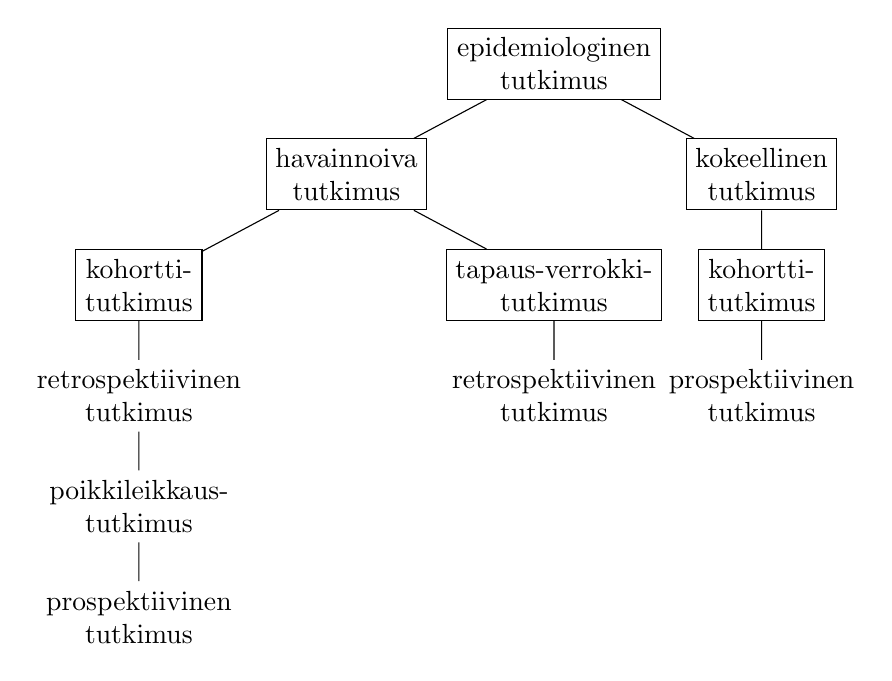
\begin{tikzpicture}
[sibling distance = 15em, level distance = 4em, every node/.style = {shape = rectangle, draw, align = center}]
\node{epidemiologinen\\tutkimus}
   child{node{havainnoiva\\tutkimus}
        child{node{kohortti-\\tutkimus}
            child{node[draw=none,fill=none]{retrospektiivinen\\tutkimus}
                child{node[draw=none,fill=none]{poikkileikkaus-\\tutkimus}
                    child{node[draw=none,fill=none]{prospektiivinen\\tutkimus}}}}}
        child{node{tapaus-verrokki-\\tutkimus}
            child{node[draw=none,fill=none]{retrospektiivinen\\tutkimus}}}}
    child{node{kokeellinen\\tutkimus}
        child{node{kohortti-\\tutkimus}
            child{node[draw=none,fill=none]{prospektiivinen\\tutkimus}}}};
\end{tikzpicture}
\caption{Epidemiologiset tutkimusasetelmat, \cite{twisk13}}
\label{fig:epikaavio}
\end{figure}

\subsection{Pitkittäisaineiston analyysi}
\label{sub:pitkittaisanal}

Kuten sanottu, pitkittäisaineistoille on ominaista yhden tai useamman yksilön seuranta usean havaintokerran ajan. Käytännössä useinkaan kaikilta yksilöiltä ei kyetä saamaan samaa määrää havaintoja ja havaintoajankohdat voivat vaihdella. Tällöin puhutaan epätasapainoisesta (\textit{unbalanced}) pitkittäisaineistosta \cite{laird82}.

Mm. \cite{verbeke00, goldstein11} mukaan epätasapainoisen pitkittäisaineiston analyysissa ei suoraan voida hyödyntää yleistä monimuuttujamenetelmien kehikkoa, vaan malli tulee jakaa kahdelle tai useammalle tasolle. 

Samoilta yksilöiltä kerättyjen toistettujen mittausten muodostamassa pitkittäisaineistossa yksilökohtaiset mittausvektorit muodostavat hierarkian ensimmäisen tason ja itse yksilöt toisen tason \cite{goldstein11}.

%Ensimmäisellä tasolla yksilökohtaisten toistomittaussarjojen vektorit tiivistetään pienempään [EPÄMÄÄRÄINEN KÄÄNNÖS] määräänhttps://www.overleaf.com/project/5d7b3ded96d15900017b8b7e yksilökohtaisia regressiokertoimia ja toisella tasolla estimaatit liitetään tunnettuihin taustamuuttujiin hyödyntäen monimuuttujamenetelmiä.

Lineaaristen sekamallien kirjallisuudessa kaksitasoisen lähestymistavan perusteoksena viitataan \cite{laird82} artikkeliin \textit{Random-Effects Models for Longitudinal Data}. Tosin \cite{laird82} esittävät tasot yhtenä lineaarikombinaationa ja vasta myöhemmässä kirjallisuudessa mm. \cite{verbeke00, talbott06} on katsottu luontevaksi esitellä ensin kaksitasoinen malli ja johtaa siitä \cite{laird82} yleinen lineaarisen sekamallin muoto.

Palaamme kaksitasoisen mallin ja yleisen lineaarisen sekamallin määritelmään myöhemmin. [ks LSM]. \\

\subsection{Finlapset aineisto}
\label{sub:finlapsetdata}

Tutkielmassa hyödynnetty aineisto perustuu Terveyden ja hyvinvoinninlaitoksen (THL) Finlapset-rekisterihankkeen (FINLAPSET) ohessa kerättyihin tietoihin lasten ja nuorten  perustuvat lastenneuvoloiden kouluterveydenhuollon ja opiskelijaterveydenhuollon terveydenhoitokäynneillä suoritetuista paino- ja pituusmittauksista. Tiedot on kerätty osana perusterveydenhuollon avohoidon hoitoilmoitusrekisterin (Avohilmo) tietokeräystä.\\

Terveystarkastuksissa kerättävistä tiedoista pituus- ja painotiedot ovat olleet osa Avohilmon tietosisältöä vuodesta 2010 lähtien, mutta tietopuutteiden vuoksi tässä tutkielmassa on mukana tietoja vuodesta 2013 alkaen. \\

Finlapset-rekisterihankkeen keskeisiä tutkimuskysymyksiä olivat lasten ja nuorten ylipaino ja lihavuus sekä pituus- ja painotietojen valtakunnallinen kattavuus. Tarkastelemme seuraavaksi aineiston keskeisiä rajauksia ja teknisiä määrityksiä. \\

\subsubsection{Finlapset-aineiston muodostus}
\label{ssb:finlapsetdatamuod}

Avohilmosta suoritetun poiminnan yhteydessä aineistoon on tehty seuraavat rajaukset:

\begin{itemize}
    \item Käynti on tehty vastaanotolla
    \item Käynti on luonteeltaan terveydenhoitokäynti
    \item Käynti on luokiteltu lastenneuvola-, kouluterveydenhuolto-, opiskelijaterveydenhuoltokäynniksi
    \item Lapsen tai nuoren ikä mittaushetkellä on välillä $[1,75;20)$
\end{itemize}

Rajauksillä on pyritty poistamaan mahdollisia harhan lähteitä. Esimerkiksi rajaamalla tarkastelu vain terveydenhoitokäynteihin voidaan sulkea pois sellaisia käyntejä, jotka liittyvät jonkin sairauden hoitoon tai seurantaan. Näillä lapsilla käyntejä voi olla huomattavasti enemmän kuin vertaisillaan ja joihinkin sairauksiin voi myös liittyä epätavallisia painon muutoksia. \\

Paino- ja pituustietojen kirjaaminen tapahtuu sähköisesti potilastietojärjestelmiin, joista ne siirretään osaksi Avohilmoa. Kirjaamiskäytännöt vaihtelevat potilastietojärjestelmittäin ja pituus- ja painomittaukset voivat olla kirjattu eri yksiköissä sekä niissä voi olla inhimillisestä kirjausvirheitä.\\

Edellämainittuja on pyritty karsimaan seuraavilla yksinkertaisilla skaalaussäännöillä:

\begin{itemize}
    \item Paino yli 1000 $\longrightarrow$ yksikkönä g?  $\longrightarrow$ jaetaan 1000:lla kunnes alle 1000
    \item Pituus on yli 300 $\longrightarrow$ yksikkönä mm? $\longrightarrow$ jaetaan 10:llä kunnes alle 300
    \item Pituus pienempää kuin 2,3 $\longrightarrow$ yksikkönä m? $\longrightarrow$ kerrotaan 100
\end{itemize}

Aineistosta rajattiin pois myös biologisesti mahdottomiksi tulkitut mittaukset. Tämä suoritettiin laskemalla painosta ($w$) ja pituudesta ($h$) ensin niiden keskinäistä suhdetta kuvaava painoindeksi (\textit{Body Mass Index, BMI}) tavanomaisella kansainvälisesti vakiintuneella menetelmällä

$$
\textbf{BMI} = \frac{w_{kg}}{h_{m}^2}.
$$

Lapsen ruumiinrakenne, ja siten painon ja pituuden suhde, vaihtelee huomattavasti iän mukaan, joten lapsen iän mukaisen painoindeksin jakauman ääriarvoja voidaan arvioida Colen LMS-menetelmällä \cite{cole90}. LMS-menetelmä, joskus myös \textit{BMI z-score function}, tarjoaa potenssimuunnoksella normalisoidun ja standardisoidun keskihajontapistemäärän, perustuen lapsen kuukausi-iän ja sukupuolen perusteella muodostettuihin parametreihin. Pistemäärä määritellään

$$
\text{BMI}_z = \frac{\bigg( \big( \frac{\text{BMI}}{\mu}\big)^\lambda - 1 \bigg)}{\lambda \ \sigma},
$$

jossa $\lambda$ on jakaumaa normalisoivan potenssimuunnoksen (\textit{Box Cox}) parametri, $\mu$ BMI jakauman odotusarvo ja $\sigma$ jakauman variaatiokerroin. Taulukoidut parametrit ovat saatavilla esimerkiksi Maailman terveysjärjestö WHO:lta ja Yhdysvaltain tautikeskus CDC:ltä.\\

Esimerkiksi 11-vuotiaan pojan taulukoiduilla parametreilla, $\lambda = -1,7862$, $\mu = 16,9392$ ja $\sigma = 0,11070$, painoindeksiä 34 $\frac{kg}{m^2}$ vastaava $\text{BMI}_z$ olisi

$$
\frac{\bigg( \big( \frac{34}{16,9392}\big)^{-1,7862} - 1 \bigg)}{16,9392 \cdot 0,11070} \approx 3,6,
$$

mutta vaikkapa kirjauksessa tapahtuneen näppäilyvirheen takia kirjattu painoindeksi 43 tuottaisi pistemääräksi noin 4,1.\\

Finlapset -hankkeessa kriittiseksi rajaksi valittiin $|\text{BMI}_z| = 4$ ja sitä poikkeavammat mittaukset rajattiin poiminnan ulkopuolelle.\\

LMS-menetelmää on kritisoitu, kuten yllä havaittiin, mm. siitä, että se kuvaa leveän painoindeksiarvojoukon hyvin kapealle välille. Lisäksi vanhemmilla lapsilla äärimmäisenkin korkeat painoindeksiarvot kuvautuvat hyvin lähelle hyväksyttäviksi katsottuja painoindeksin arvoja \cite{flegal13, cdc13}. \\

\cite{flegal13} suosittelevat käyttämään modifioitua pistemäärää, jossa etäisyys jakauman odotusarvosta kuvataan takaisin painoindeksiavaruuteen. Tätä on syytä punnita kehitystarpeena myös Finlapset-hankkeen tulevissa lasten ja nuorten pituus- ja painotietoja käsittelevissä julkaisuissa. \\

Finlapset-hankkeessa havaintoja rajattiin lisäksi siten, että lapsilta ja nuorilta valittiin kunkin tutkimuksessa mukana olleen kalenterivuoden syntymäpäivää lähinnä ollut mittaus. Mikäli yhtäkään mittausta ei ollut 180 vuorokauden absoluuttisella etäisyydellä kalenterivuoden syntymäpäivästä, ei kyseiselle lapselle otettu mittausta mukaan kyseiseltä kalenterivuodelta. \\

Tulokset julkaistiin vuosilta 2014\textendash2018 sellaisilta lapsilta ja nuorilta, jotka olivat mittaushetkellä 2\textendash16-vuotiaita. \\

Tässä tutkielmassa noudatetaan Finlapset-aineiston rajauksia muilta osin, lukuunottamatta rajausta yhteen mittaukseen kalenterivuotta kohden tai julkaisun yhdeydessä suoritettua kalenterivuoden ja iän perusteella tehtyä rajausta. Tutustumme aineistoon seuraavaksi yksinomaan tämän tutkielman piirissä.\\

\subsubsection{Rekisteripohjainen lasten ja nuorten neuvola-ja kouluterveysaineisto pitkittäisaineistona}
\label{ssb:rekpitkittais}

Esittäessämme FinLapset aineiston formaalisti pitkittäisaineiston muodossa, voimme, \cite{fitzmaurice11} esitystapaa mukaillen, aloittaa määrittelemällä painoindeksin satunnaismuuttujana $Y_{ij}$ ja aineistosta havaitun arvon $y_{ij}$, jossa $i = 1, \dots, N$ on yksilöön viittaava indeksi ja $j = 1, \dots n_i$ yksilön $i$ mittaukseen viittava indeksi. On tärkeää huomioida, että Finlapset aineistossa lasten mittausmäärät vaihtelevat yksilöittäin, eli on mahdollista, että $n_i \neq n_k$, kun $i,k = 1,\dots, N$ ja $i \neq k$. Finlapset aineisto on siten epätasapainoinen pitkittäisaineisto.\\

Yksilön $i$ painoindeksejä vastaavan satunnaismuuttujan vektori voidaan kirjoittaa $n_i \times 1$ matriisina

$$
\bm{Y}_i = 
\begin{bmatrix}
Y_{i1} \\
Y_{i2} \\
\vdots \\
Y_{in_i} \\
\end{bmatrix}
$$

Mittausajankohta Finlapset aineistossa on käynnin päivämäärä, jolla pituus- ja painomittaus on tehty. Tästä seuraa, että yksilöitä ei ole välttämättä mitattu samoin ajankohtina. Siten eräs ehdokas mittausajankohdaksi on yksilön $i$ $j$:nnen mittauksen päivämäärä $t_{\text{PVM}_{ij}}$.\\

Pitkittäisaineiston aikaskaala voidaan määritellä muillakin tavoin, esimerkiksi lapsen mittausajankohdan desimaali-iän mukaan, jolloin $t_{\text{IKÄ}_{ij}} = \frac{t_{\text{PVM}_{ij}} - t_{\text{SPVM}_{i}}}{365,25}$, jossa $t_{\text{SPVM}_{i}}$ on yksilön $i$ syntymäpäivä. Jakajana käytetään lukua 365,25, jolla pyritään huomioimaan karkausvuoden vaikutus.\\ 

Mittauksiin voi liittyä myös taustatietoja, jotka voivat olla aika-invariantteja (\textit{time invariant}), kuten biologinen syntymäsukupuoli ja -kunta tai ajassa muuttuvia (\textit{time variant}), kuten aika ensimmäisestä mittauksesta tai mittaushetken asuinkunta.\\

Vasteeseen $Y_{ij}$ liittyvät taustatiedot voidaan kirjoittaa $p \times 1$ taustamuuttujavektorina. \\

$$
\bm{X}_{ij} = 
\begin{bmatrix}
X_{ij_{1}} \\
X_{ij_{2}} \\
\vdots \\
X_{ij_{p}} \\
\end{bmatrix},
$$

jossa $i = 1, \dots, N$ ja $j = 1, \dots n_i$. \\ 

Yksilön $i$ taustamuuttujavektorit voidaan kirjoittaa siistimmin matriisina

$$
\bm{X}_{i} = 
\begin{bmatrix}
X_{i_{1}}^\top \\
X_{i_{2}}^\top  \\
\vdots \\
X_{i_{n_i}}^\top  \\
\end{bmatrix}
=
\begin{bmatrix}
X_{i_{11}} & X_{i_{11}} & \dots & X_{i_{1p}} \\
X_{i_{21}} & X_{i_{22}} & \dots & X_{i_{1p}} \\
\vdots & \vdots & \ddots & \vdots \\
X_{i_{n_i1}} & X_{i_{n_i2}} & \dots & X_{i_{n_ip}} \\
\end{bmatrix}
$$\\

Tarkastelemme seuraavaksi FinLapset-aineistoa tämän tutkielman kehikossa.\\

\subsubsection{FinLapset-aineiston kuvaileva tarkastelu}
\label{ssb:kuvailu}

Tutkielman keskeinen kohde on lineaaristen sekamallien soveltuvuuden tarkastelu analyysin kohteen ollessa rekisteriaineistosta muodostettu pitkittäisaineisto. Siten kysymykset liittyvät aineistossa esiintyviin ilmiöihin tilastollisten mallien sovellettavuuden ja toiminnan näkökulmasta.\\

Rekisteriaineistona FinLapset-aineisto sisältää useita tunnettuja ja tuntemattomia harhan ja mittausvirheen lähteitä, mm. tietojen puuttuminen eräiden kuntien osalta ja aineiston edustavuuden vahvistamattomuus. Tällaiset tarkastelut ja korjaavat toimenpiteet on tässä tutkielmassa pitkälti sivuutettu ja siten tämän tutkielman piirissä aineiston perusteella sen taustalla olevasta ilmiöstä tehtävien johtopäätösten suhteen tulee suorittaa varovaisuutta. \\ 

\textbf{Tutkielman aineisto}

Alkuperäinen FinLapset-aineisto käsittää painoindeksihavaintoja aikaväliltä 2.1.2013\textendash9.4.2020. Alkuperäisen aineiston tunnuslukuja on selvyyden vuoksi merkitty tähdellä (*). \\

Havaintoja on kaikkiaan $N* = 718080$ yksilöltä ja mittausten kokonaismäärä $n* = \sum\limits_{i = 1}^{N*} n_{i} = 2768012$. \\

Yksilökohtaisissa mittausten määrissä $n_{i}$ on merkittävää vaihtelua. Mittausten yksilökohtaisten määrien mediaani on 4, kvartiiliväli $[2,5]$ ja vaihteluväli $[1,116]$. \\

\begin{table}[ht]
\centering
\begin{tabular}{lrr}
\toprule
$n_i$ & N*\\
\midrule
1 & 136319\\
2 & 103017\\
3 & 103836\\
4 & 107896\\
5 & 100783\\
\addlinespace
6 & 79459\\
7 & 46876\\
8 & 21040\\
9 & 8420 \\
\addlinespace
10-29 & 10333\\
30- & 101\\
\bottomrule
\end{tabular}
\caption{FinLapset-aineiston yksilökohtaisten mittauslukumäärien jakauma}
\label{table:mittausmaarat}
\end{table}

Mittausten määrien jakaumista (Taulukko ~\ref{table:mittausmaarat}) huomaamme, että suurimman yksittäisen ryhmän muodostavat yksilöt, joilla on vain yksi mittaus. Tämä on syytä huomioida, sillä yleisesti pitkittäisaineiston oletetaan sisältävän yksilöä kohden vähintään kaksi mittausta \cite{west14}. Yksilöitä, joilla on yli 30 mittausta on koko ainestossa vain 101 kappaletta. \\\\

Tutkielman soveltavassa vaiheessa tehtyjen havaintojen (REF!!) perusteella todettiin alkuperäisen FinLapset-aineiston analyysiin vaadittujen menetelmien laajentavan tämän tutkielman sille asetetun vaativuustason mukaisten rajausten ulkopuolelle. Kompromissina alkuperäisen FinLapset-aineston sijaan tutkielman aineisto rajoittuu yksilöihin, joiden kotikuntana on kunkin kalenterivuoden lopussa ollut Helsinki. Yksilöiltä, joiden kotikunta on muuttunut seuranta-aikana, otetaan kuitenkin mukaan kaikki saatavilla olevat mittaukset.\\

Täten aineiston määrää saatiin rajattua niin, että tarvittavien mallien sovittaminen onnistuu sellaisilla välinellä, joiden esittely katsotaan tämänkaltaisessa tutkielmassa perustelluiksi. Tämä ei tarkoita, että keskustelu alkuperäisen aineston analysointiin tarvittavista menetelmistä sivuutetaan.\\

Tämän rajauksen lisäksi otettiin tarkasteluun mukaan vain sellaiset yksilöt, joilla on 2\textendash9 mittausta, sillä yksilöiden merkittävä osuus, joilla on vain yksi mittaus, vaikutti huomattavasti optimointialgoritmien toimintaan (REF).\\

Tulee kuitenkin painottaa, että rajauksenkin jälkeen aineisto sisältää huomattavan määrän havaintoja suureltä määrältä yksilöitä ja se mahdollistaa samankaltaisten haasteiden kohtaamisen kuin alkuperäinen FinLapset-aineisto.\\

Tutkielman rajatussa aineistossa havaintoja on kaikkiaan $N = 101239$ yksilöltä ja mittausten kokonaismäärä $n = \sum\limits_{i = 1}^{N} n_{i} = 421660$. \\

\begin{table}[ht]
\centering
\begin{tabular}{lr}
\toprule
$n_i$ & $N$\\
\midrule
2 & 20168\\
3 & 21115\\
4 & 20186\\
5 & 17070\\
\addlinespace
6 & 12144\\
7 & 6586\\
8 & 2811\\
9 & 1159\\
\bottomrule
\end{tabular}
\caption{Tutkielman rajatun aineiston yksilökohtaisten mittauslukumäärien jakauma}
\label{table:mittausmaaratrajattu}
\end{table}

Vaikka yksilökohtaisten mittausmäärien vaihteluväli pieneni (Taulukko ~\ref{table:mittausmaaratrajattu}), mediaani ja kvartiiliväli pysyivät samana. \\

\textbf{Tutkielman aineston muuttujat}\\

Tutkielmassa hyödynnetään seuraavia FinLapset-aineiston muuttujia

\begin{itemize}
    \item Yksilön pseudonymisoitu tunniste
    \item Käynnin päivämäärä
    \item Biologinen sukupuoli
    \item Syntymäpäivämäärä
    \item Painoindeksi
\end{itemize}

Sukupuolijakauma (Taulukko ~\ref{table:sukupuolijakauma}) vaikuttaa kuvaavaan likimain Suomen väestöä, jossa tyttöjen osuus on hieman poikien osuutta pienempi.\\

\begin{table}[H]
\centering
\begin{tabular}{rr}
\toprule
Sukupuoli & N\\
\midrule
Tytöt & 49837\\
Pojat & 51402\\
\bottomrule
\end{tabular}
\caption{FinLapset-aineiston sukupuolijakauma}
\label{table:sukupuolijakauma}
\end{table}

Tutkielman aineistossa esiintyy kolme kiinnostavaa aikadimensiota. Ensimmäinen näistä on yksilön ikä mittaushetkellä, toinen on aika, jolloin mittaus on suoritettu ja kolmas on syntymäkohortti. Näillä dimensioilla on muihin muuttujiin verrattuna poikkeuksellinen ominaisuus, sillä kunkin dimension voi yksikäsitteisesti päätellä kahdesta muusta. Nämä dimensiot muodostavat ikä-periodi-kohortti-ilmiön, jota on analysoitu myös lineaaristen sekamallien kirjallisuudessa \cite{yang06}.\\

Tämän tutkielman osalta kiinnitämme huomion kahteen dimensioon, mittausaikaan ja yksilön ikään mittaushetkellä. Näitä voi luontevasti kuvata esimerkiksi Lexis-diagrammeilla (Kuva ~\ref{fig:lexisplot}), joissa pitkittäisaineisto kuvataan yksilökohtaisina polkuina, x-akselin kuvatessa aikadimensiota ja y-akselin ikää mittaushetkellä.\\

\begin{figure}[H]
\centering
  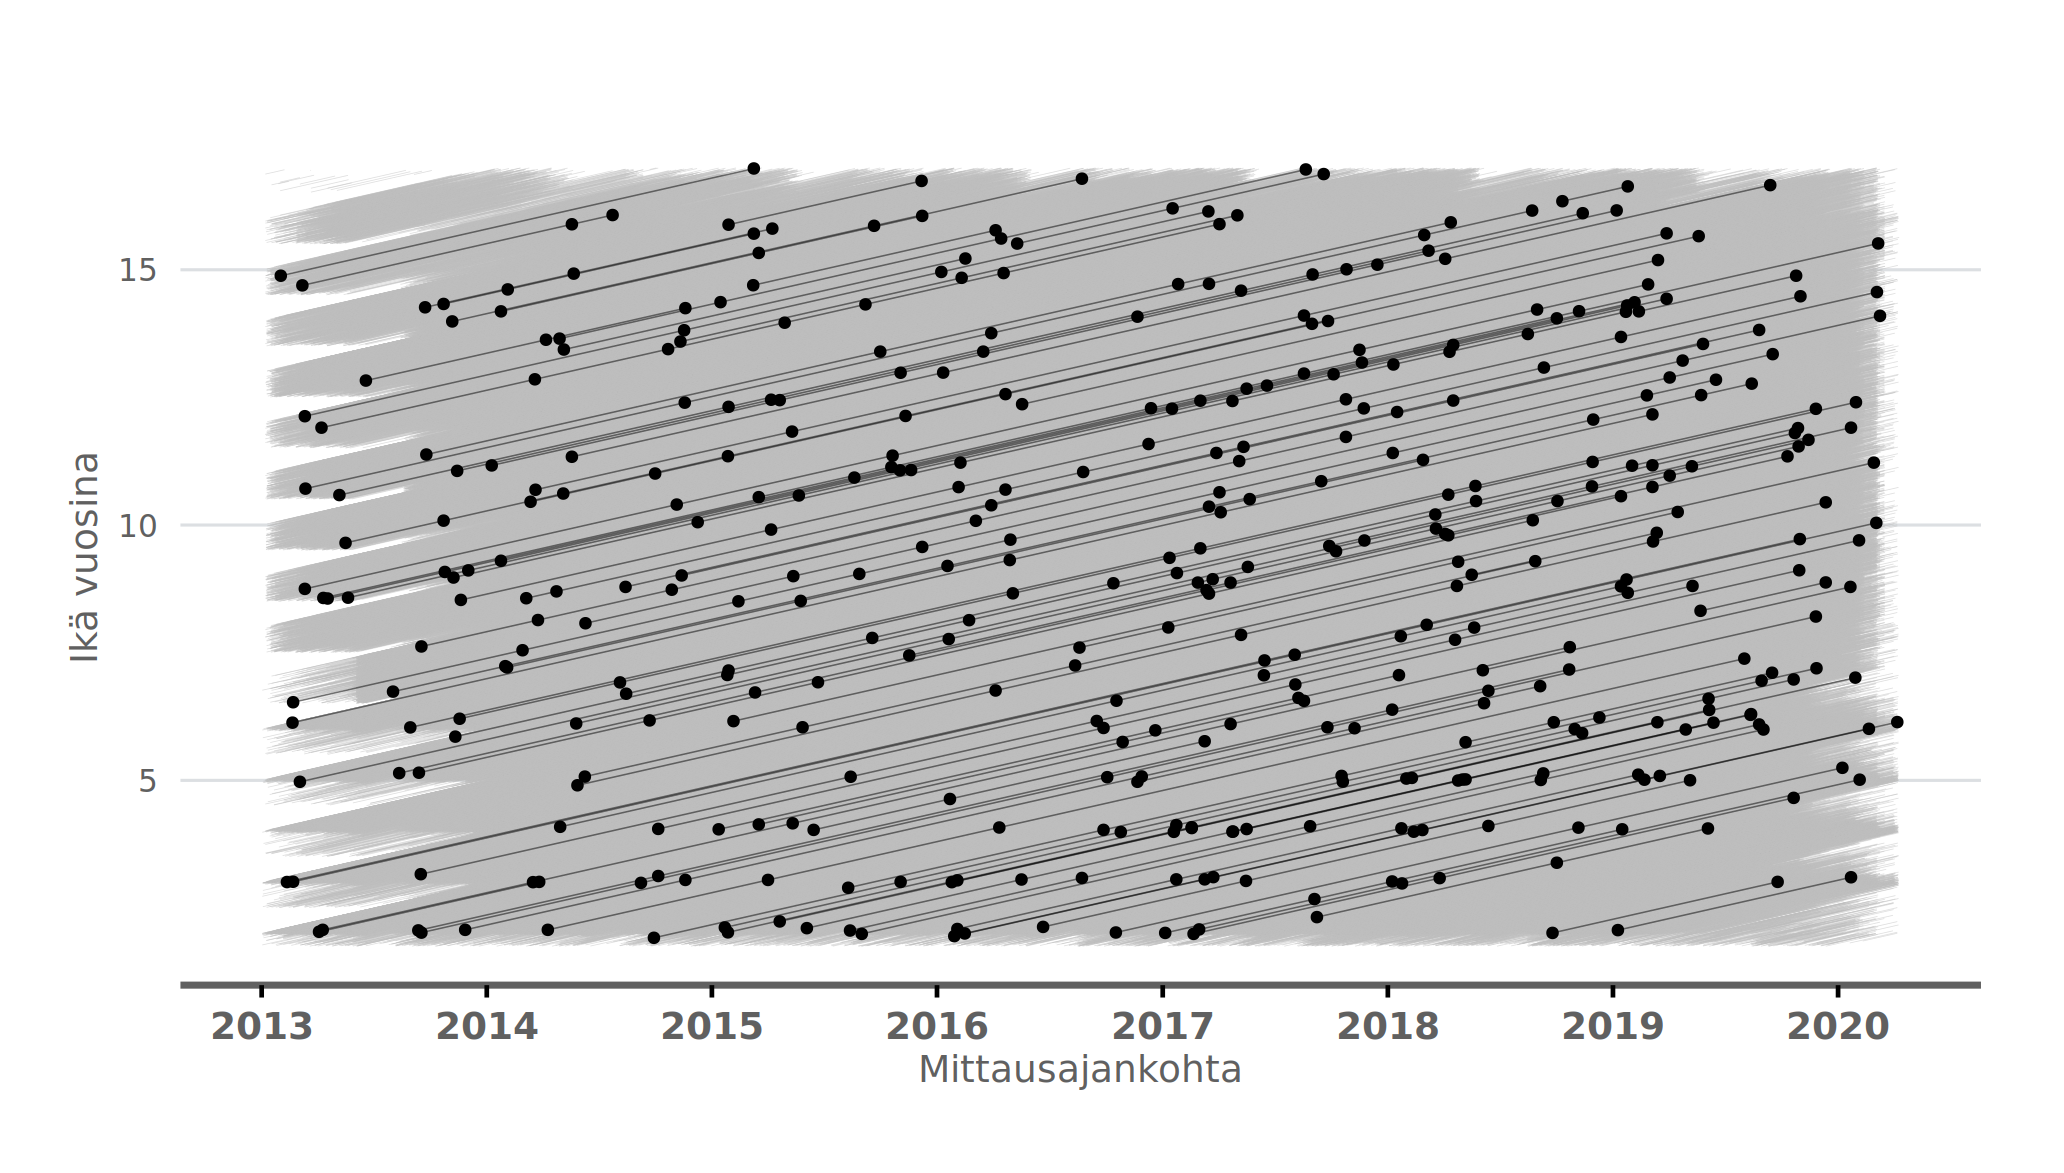
\includegraphics[scale=0.8]{kuvaajat/lex_plot.png}
  \caption{Lexis-diagrammi mittauksen päivämäärän ja mittaushetken iän mukaan. Kaikkien yksilöiden mittausaikajanat esitetty harmaana. Sadan satunnaisesti valitun yksilön mittausaikajanoja on havainnollistettu mustalla ja yksittäisiä mittausajankohtia mustilla palloilla.}
  \label{fig:lexisplot}
\end{figure}

Tärkeimpänä muuttujana tarkastelemme viimeiseksi vastemuuttuja painoindeksiä. Painoindeksin jakauma (Kuva ~\ref{fig:bmi_dens}) vaikuttaa olevan positiivisesti vino. Tämä ei kuitenkaan välttämättä ole ongelma, sillä normaalisuusoletus koskee yksinomaan jäännösvirheitä \cite{west14}. Vaikka vastemuuttujan ja jäännösvirheiden jakaumat ovat lineaaristen mallien tapauksessa analogisia \cite{fitzmaurice11}, lineaaristen sekamallien tapauksessa tarkastelemme yksilön toistettujen mittausten jäännösvirheitä.\\

\begin{figure}[ht]
\centering
  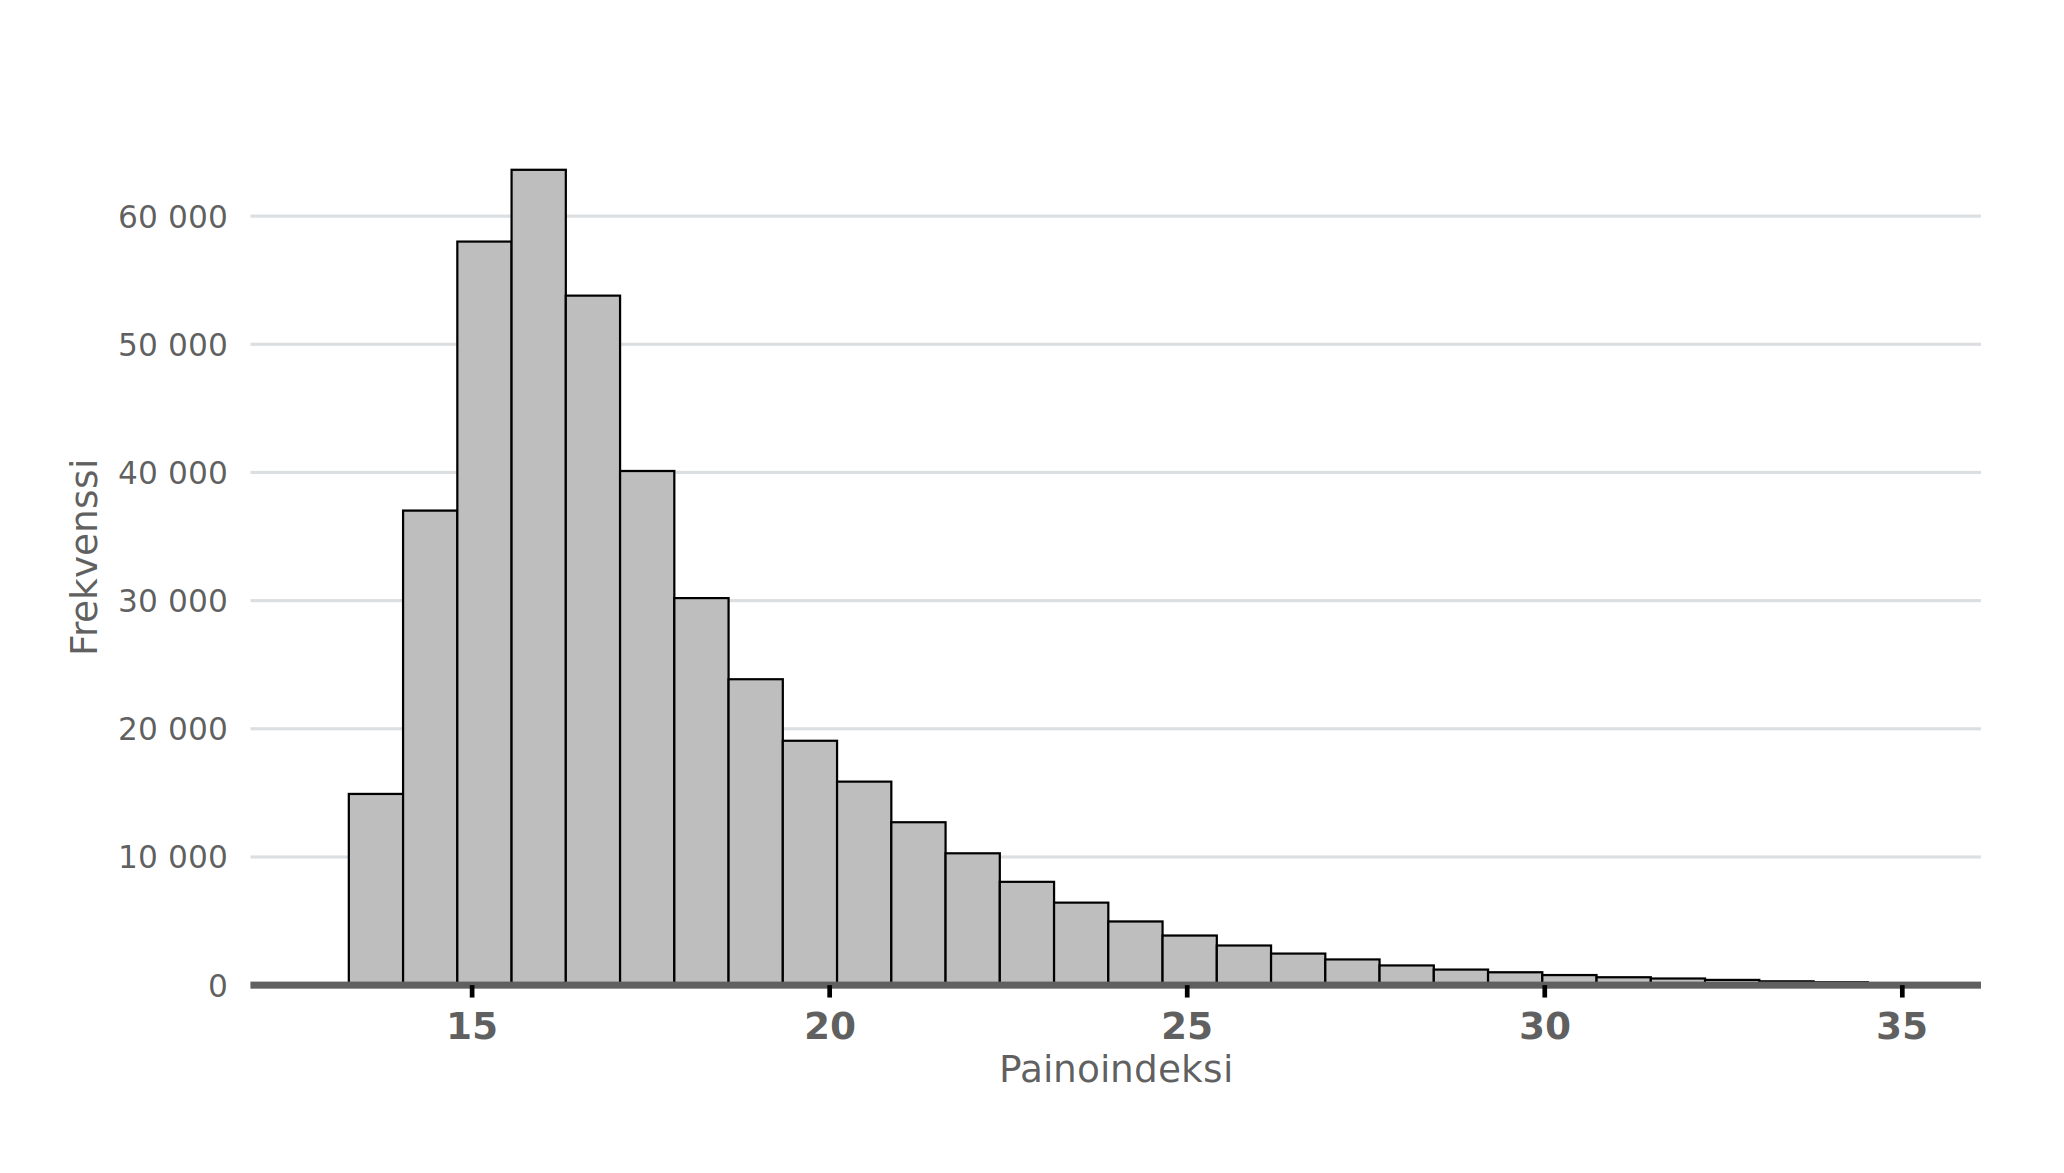
\includegraphics[scale=0.8]{kuvaajat/bmi_dens.png}
  \caption{Painoindeksihavaintojen empiirinen jakauma}
  \label{fig:bmi_dens}
\end{figure}

Toisin sanoen, kunkin yksilön havaintoihin sovitetun lineaarisen mallin (Kuva ~\ref{fig:xyplot}) jäännösvirheiden tulisi noudattaa yksiulotteista normaalijakaumaa. Kuvasta huomaamme, että yksilöiden välillä on huomattavasti vaihtelua, mutta yksittäisen yksilön kohdalla oletus painoindeksin ja iän yhteyden lineaarisuudesta vaikuttaisi alustavasti perustellulta.\\

\begin{figure}[H]
\centering
  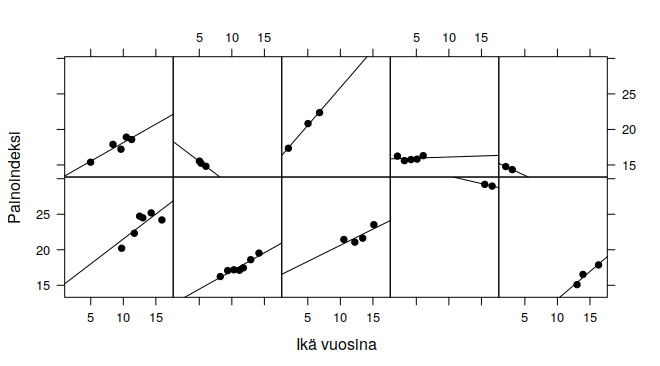
\includegraphics[scale=0.8]{kuvaajat/xyplot.png}
  \caption{Kymmenen satunnaisesti valitun yksilön painoindeksimittaukset yksinkertaisille lineaarisilla sovitesuorilla}
  \label{fig:xyplot}
\end{figure}

\section{Lineaarinen sekamalli}
\label{sec:lsm}

Lineaariset sekamallit (LSM) ovat tilastollisten mallien joukko lähtökohtaisesti jatkuville vastemuuttujille, joiden jäännösvirheet (residuaalit) ovat normaalisti jakautuneita, mutta eivät välttämättä riippumattomia tai niiden varianssi ei ole vakio \cite{west14}. Kyseisten mallien joukkoa kuvaava, yleisesti käytössä oleva englanninkielinen nimi \textit{linear mixed (effect) model}, juontuu mallien ominaisuuksista siten, että mallit ovat parametreiltään lineaarisia ja niihin voi liittyä taustamuuttujien muodossa sekä \textit{kiinteitä} (\textit{fixed}) ja \textit{satunnaisia} (\textit{random}) vaikutuksia (\textit{effects}) \cite{west14}.

\cite{laird82} kuvaavat kiinteiden ja satunnaisvaikutusten yhteyttä seuraavalla tavalla: Olkoon toistettujen mittausten yksilökohtaiset todennäköisyysjakaumat samaa muotoa (\textit{form}) kaikille yksilöille, mutta sallittakoon näiden todennäköisyysjakaumien parametrien vaihtelu yksilöiden välillä. Näiden populaation \textit{satunnaisvaikutusten} parametrien jakauma muodostaa mallin toisen tason.

Siirtääksemme \cite{laird82} esittämän esimerkin FinLapset-aineiston kehikoon oletamme siis, että yksittäisen lapsen painoindeksin ja valittujen taustamuuttujien (esimerkiksi ikä, sukupuoli jne.) välinen yhteys on lineaarinen, mutta kutakin lasta kohden sovitetun lineaarisen regression parametrit voivat vaihdella. Siten, ehdollisesti yksittäisen lapsen parametrejä kohtaan ja, että populaation regressioparametrit noudattavat 2-ulotteista normaalijakaumaa, toistettujen mittausten reunajakauma noudattaa moniulotteista normaalijakaumaa asetelmaa vastaavalla kovarianssirakenteella. 

\subsection{Lineaarisen sekamallin määritelmä}
\label{sub:lsmmaar}

Jotta voimme perusteellisesti ymmärtää lineaarisen sekamallin luonteen, aloitamme tarkastelun hyvin yleisestä tilastollisen mallin esitysmuodosta, yksinkertaisesta lineaarisesta regressiomallista mallista.

\subsubsection{Lineaarinen regressio}
\label{ssb:linreg}

Olkoon $y_i$ satunnaismuuttujan $Y_i$ havaittu arvo, $x_i$ satunnaismuuttujan $X_i$ havaittu arvo, $\beta_0$ (vakiotermi) ja $\beta_1$ (taustamuuttujan $x_i$ regressiokerroin) kiinteät, mutta tuntemattomat regressiokertoimet ja satunnaismuuttuja $\epsilon_i$ mallin selittämätön osa (jäännöstermi) havainnoille $i = 1,\dots,n$.

Satunnaismuuttujan $Y_i$ ja taustamuuttujan $x_i$ yhteyttä kuvaa yksinkertainen lineaarinen regressiomalli

$$
Y_i = \beta_0 + \beta_1 x_i + \epsilon_i
$$

Laajennettuna useaan usean taustamuuttujan lineaariseen regressioon edellinen voidaan esittää muodossa

$$
Y_i = \beta_0 + \beta_1 x_{i1} + \dots + \beta_p x_{ip} + \epsilon_i
$$

Tiivistääksemme edellistä muotoa, voimme määritellä sarakevektorit $\bm{x_i} = [x_i1 , \dots, x_{ip}]^\top$ ja $\bm{\beta} = [\beta_1 , \dots, \beta_{p}]^\top$ ja kirjoittaa mallin muodossa

$$
Y_i = \bm{x_i}^\top \bm{\beta} + \epsilon_i
$$

havainnoille $i = 1,\dots,n$. \\

%[TARPEETON?] Lopuksi voimme tiivistää mallia edelleen määritellen kullekkin mallin termille havaintokohtaiset vektorit

%$$
%\begin{aligned}
%\begin{bmatrix} 
%Y_1 \\
%\vdots \\
%Y_n \\
%\end{bmatrix}&=
%\begin{bmatrix} 
%\bm{x}_1^\top \\
%\vdots \\
%\bm{x}_n^\top \\
%\end{bmatrix}
%\begin{bmatrix} 
%\beta_1 \\
%\vdots \\
%\beta_p \\
%\end{bmatrix}&&+
%\begin{bmatrix} 
%\epsilon_1 \\
%\vdots \\
%\epsilon_n \\
%\end{bmatrix} \\
%\bm{Y}\quad&=\quad \bm{X}\bm{\beta}&&+\quad \bm{\epsilon}
%\end{aligned}
%$$

[VIELÄ YKSI VÄLIVAIHE? ESIM \cite{fitzmaurice11} s. 76 HISTORICAL APPROACHES; repeated measures anova]


Seuraavaksi hyödynnämme lineaarisen mallin määritelmää esitellessämme lineaariselle sekamallille ensin kaksitasoisen mallin, jonka jälkeen etenemme luontevasti tasot yhdistävään \cite{laird82} yleiseen lineaariseen sekamalliin.

\subsubsection{Kaksitasomalli}
\label{ssb:kaksitaso}

Monitasomalleille keskeistä on aineiston hierarkkisen rakenteen huomioiminen mallissa \textit{satunnaisvaikutusten} avulla \cite{talbott06}. Pitkittäisaineistoa kuvaavassa kaksitasomallissa hierarkian ensimmäinen taso käsittää yksilön mittauskertojen välisen vaihtelun ja toinen taso yksilöiden välisen vaihtelun. Monitasomallit voidaan yleistää myös useammalle tasolle \cite{goldstein11, burzykowski13}.

\paragraph{Ensimmäinen taso}\mbox{}\\

Ensimmäisellä tasolla oletamme kunkin yksilön keskimääräisen vasteen (\textit{Mean response}) noudattavan lineaarista regressiomallia samoilla taustamuuttujilla, mutta yksilöllisillä regressiokertoimilla \cite{fitzmaurice11}. 

Edellistä mukaillen, voimme esittää ensimmäisen tason muodossa

$$
\bm{Y}_i = \bm{Z}_i \bm{\beta}_i + \bm{\epsilon}_i,
$$

jossa $\bm{Y}_i$ on yksilön $i$ $n_i$-vastevektori, $\bm{\beta}_i$ tuntemattomat regressiokertoimet sisältävä $q$-vektori ja $\bm{Z}_i \bm{\beta}_i$ yksilön $i$ tuntematon keskimääräinen vasteen kehitys (\textit{Response trajectory}). Ensimmäisen tason kontekstissa matriisi $\bm{Z}_i$ määrittelee kuinka yksilön keskimääräinen vaste muuttuu ajassa, mutta määritelmä tulee vaatimaan tarkennusta.

Niin sanottujen yksilöiden välillä vaihtelevien kiinteiden, mutta tuntemattomien vaikutusten lisäksi ensimmäiseen tasoon liittyy myös yksilön $i$ mittauksia koskeva satunnaisvirhe $\bm{\epsilon_i}$, jossa $\bm{\epsilon_i} \sim N(0,\bm{R}_i)$, jossa $\bm{R}_i$ on jokin $n_i \times n_i$ kovarianssimatriisi. Yksinkertaisuuden vuoksi voimme olettaa, että $\bm{R}_i = \sigma^2\bm{I}_{n_i}$

Kuvataksemme täsmällisemmin mallin osia, voimme esittää mallin yksilön $i$ vastelle aukikirjoitettussa matriisimuodossa

$$
\begin{bmatrix}
Y_{i1} \\
\vdots \\
Y_{in_{i}} \\
\end{bmatrix}=
\begin{bmatrix}
1 & t_{i1} \\
\vdots \\
1 & t_{in_{i}} \\
\end{bmatrix}+
\begin{bmatrix}
\beta_{1i} \\
\beta_{2i} \\
\end{bmatrix}+
\begin{bmatrix}
e_{i1} \\
\vdots \\
e_{in_{i}} \\
\end{bmatrix}
$$

\paragraph{Toinen taso}\mbox{}\\

Toisella tasolla tuomme malliin oletuksen, että yksilökohtaiset vaikutukset $\bm{\beta}_i$ ovat satunnaismuuttujia jollakin odotusarvolla ja kovarianssilla.

Keskeistä on $\bm{\beta}_i$ yksilöiden välisen vaihtelun mallintaminen mittausajankohdasta riippumattomien vasteen yksilöllisiä eroja selittävinen taustamuuttujien funktiona \cite{fitzmaurice11}.

Siten $\bm{\beta}_i$ odotusarvoksi saamme

$$
\text{E}(\bm{\beta}_i) = \bm{K}_i \bm{\beta},
$$

jossa $\bm{K}_i$ on yksilöiden välistä vaihtelua selittävien muuttujien $(q \times p)$ matriisi.

Yksilöiden välistä residuaalivaihtelua, jota $\bm{K}_i$ ei selitä, merkitsemme

$$
\text{Cov}(\bm{\beta}_i) = \bm{G}.
$$

Lopuksi voimme yhdistää ensimmäisen ja toisen tason komponentit esittääksemme $\bm{Y}_i$:lle lineerisen sekamallin yleisen muodon \cite{fitzmaurice11, verbeke00}.

\subsubsection{Yleinen lineaarinen sekamalli}
\label{ssb:ylsm}

Yhdistääksemme ensimmäisen ja toisen tason, hyödyntäen toisen vaiheen oletuksia, voimme kirjoittaa $\bm{\beta}_i$ uudelleen muodossa

$$
\bm{\beta}_i = \bm{K}_i \bm{\beta} + \bm{b}_i,
$$

jossa $\bm{b}_i \sim N(0,\bm{G})$ \\

Tässä $\bm{b}_i$ kuvaa $i$:nnen yksilön poikkeamaa keskimääräisestä vasteesta, kun yksilöiden yhteiset taustamuuttujat on huomioitu \cite{fitzmaurice11}.

Yhdistetty muoto saadaan sijoittamalla

$$
\begin{aligned}
\bm{Y}_i &= \bm{Z}_i \bm{\beta_i} + \bm{\epsilon}_i \\
&= \bm{Z}_i (\bm{K}_i \bm{\beta} + \bm{b}_i) + \bm{\epsilon}_i \\
&= (\bm{Z}_i \bm{K}_i) \bm{\beta} + \bm{Z}_i \bm{b}_i + \bm{\epsilon}_i \\
&= \bm{X}_i \bm{\beta} + \bm{Z}_i \bm{b}_i + \bm{\epsilon}_i, \\
\end{aligned}
$$

jossa $\bm{X}_i = \bm{Z}_i \bm{K}_i$. \\

Yleisesti muotoiltuna, malli joka tyydyttää vaatimukset

$$
\left\{
    \begin{array}{ll}
        \bm{Y}_i = \bm{X}_i \bm{\beta} + \bm{Z}_i \bm{b}_i + \bm{\epsilon}_i \\
        \bm{b}_i \sim N(0,\bm{G}) \\
        \bm{\epsilon}_i \sim N(0,\bm{R}_i) \\
        \bm{b}_i, \dots , \bm{b}_N \perp \bm{\epsilon}_i, \dots , \bm{\epsilon}_N 
    \end{array}
\right.
$$

on lineaarinen sekamalli \cite{verbeke00, laird82}.\\


\cite{fitzmaurice11} alleviivaavat, että kaksitasomalliin, sen ollessa pedagogisesti hyödyllinen lineaarisen sekamallin yksilöiden välisten ja yksilökohtaisten vaikutusten esitystapa, liittyy merkittävä rajoite, sillä muoto  $\bm{X}_i = \bm{Z}_i \bm{K}_i$ edellyttää, että $\bm{K}_i$ sisältää vain yksilöiden välisiä vaikutuksia selittäviä muuttujia ja $\bm{Z}_i$ vain yksilökohtaisia ajassa muuttuvia vaikutuksia selittäviä muuttujia.

Tämä rajoite on kuitenkin kierrettävissä olettamalla, että $\bm{X}_i$ on lineaarisen sekamallin mielivaltainen koematriisi ja, että $\bm{Z}_i$ muodostuu sarakkeista, jotka ovat $\bm{X}_i$ sarakkeiden osajoukko. Tällöin vasteen $\bm{Y}_i$ odotusarvo yli kaikkien yksilökohtaisten vaikutusten

$$
\text{E}(\bm{Y}_i) = \bm{X}_i \bm{\beta}, \\
$$

määrittelee vasteen keskimääräisen kehityksen koko tarkasteltavana olevalle joukolle ja $\bm{Z}_i \bm{b}_i$ kuvaa selittämättä jäänyttä osaa, eli yksilökohtaisia poikkeamia tarkastelujoukon vasteen keskimääräisestä kehityksestä \cite{fitzmaurice11}. \\

Täsmällisemmin muotoiltuna, tarkastellaan ehdollista odotusarvoa

$$
\text{E}(\bm{Y}_i | \bm{b}_i) = \bm{X}_i \bm{\beta} + \bm{Z}_i \bm{b}_i.
$$

Koska $\text{E}(\bm{b}_i) = 0$, saamme reunajakauman $\bm{Y}_i$ odotusarvoksi

$$
\begin{aligned}
\text{E}(\bm{Y}_i) &=  \text{E}(\text{E}(\bm{Y}_i | \bm{b}_i)) \\
&=  \text{E}(\bm{X}_i \bm{\beta} + \bm{Z}_i \bm{b}_i) \\
&=  \bm{X}_i \bm{\beta} + \bm{Z}_i \text{E}(\bm{b}_i) \\
&=  \bm{X}_i \bm{\beta}. \\
\end{aligned}
$$

Siten vahvistamme tulkinnan, että parametrit $\bm{\beta}$ kuvaavat koko tarkastelujoukon yhteisiä, niin kutsuttuja \textit{kiinteitä} vaikutuksia ja ottaen huomioon kiinteät vaikutukset, $\bm{b}_i$ kuvaa yksilön $i$ poikkeamaa koko tarkastelujoukon keskimääräisesta vasteesta, toisin sanoen mallin \textit{satunnaisvaikutuksia}. \\

\cite{fitzmaurice11} mukaan lineaarisen sekamallin kaksitasoesitys asettaa erityisvaatimuksia myös mallin kovarianssille. Koska kovarianssirakenteella on monin tavoin keskeinen asema, sekä yleisen lineaarisen sekamallin teoriassa, että pitkittäisaineiston erityistapauksessa, erotamme sen käsittelyn omaksi osiokseen.\\ 

\subsection{Kovarianssirakenteet}
\label{sub:kovarianssirakenteet}

Tarkastellaan seuraavaksi lineaarisen sekamallin kovarianssirakenteita \cite{fitzmaurice11} esittämässä yleisessä muodossa. Lähtökohtana on erottaa yksilökohtaisen ja yksilöiden välisen vaihtelun lähteet ja mahdollistaa näiden yksikäsitteinen analyysi.\\

Yleisen lineaarisen sekamallin

$$
\bm{Y}_i = \bm{X}_i \bm{\beta} + \bm{Z}_i \bm{b}_i + \bm{\epsilon}_i \\
$$

tapauksessa voimme, edellisessä luvussa esitetyn määritelmän mukaan, esittää yksilön $i$ keskimääräisen vasteen ehdollisena odotusarvona

$$
\text{E}(\bm{Y}_i | \bm{b}_i) = \bm{X}_i \bm{\beta} + \bm{Z}_i \bm{b}_i, \\
$$

jossa otamme huomioon yksilön $i$ poikkeaman $\bm{b}_i$ koko tutkimusjoukon keskimääräisestä vasteesta.

Pyrkimyksessämme erottaa yksilön $i$ mittausten keskinäinen vaihtelu koko tutkimusjoukon mittausten vaihtelusta, määritellään yksilön $i$ mittausten kovarianssi samaan tapaan ehdollisena kovarianssina 

$$
\text{Cov}(\bm{Y}_i | \bm{b}_i) = \text{Cov}(\bm{\epsilon}_i) = \bm{R}_i,
$$

jolloin \cite{fitzmaurice11} mukaan reunajakauman $\bm{Y}_i$ kovarianssiksi saamme

$$
\begin{aligned}
\text{Cov}(\bm{Y}_i) &= \text{Cov}(\bm{X}_i \bm{\beta} +\bm{Z}_i\bm{b}_i + \bm{\epsilon}_i) \\
&= \text{Cov}(\bm{Z}_i \bm{b}_i) + \text{Cov}(\bm{\epsilon}_i) \\
&= \bm{Z}_i \text{Cov} (\bm{b}_i) \bm{Z}^\top_i + \text{Cov}(\bm{\epsilon}_i)\\
&= \bm{Z}_i \bm{G} \bm{Z}^\top_i + \bm{R}_i.\\
\end{aligned}
$$ \\

Näin ollen, lineaarinen sekamalli mahdollistaa yksilöiden välisten varianssilähteiden $\bm{G}$ ja yksilökohtaisten varianssilähteiden $\bm{R}_i$ yksikäsitteisen analyysin. \\

Koska mallin kovarianssi esitetään mittausajankohtien funktiona, ei satunnaisvaikutusten kovarianssirakenne vaadi tasapainoista asetelmaa pitkittäisaineistossa, kovarianssiparametrien määrä ei riipu mittausajankohdista tai niiden lukumäärästä ja varianssi sekä kovarianssi voivat myös muuttua mittausajankohtien funktiona, mistä on merkittävää hyötyä epätasapainoisen pitkittäisaineiston analyysissä \cite{fitzmaurice11}. \\

Kirjoitetaan yksilöiden välisten satunnaisvaikutusten $q$-vektori $\bm{b}_i \sim N(0,\bm{G})$ yksilölle $i$ matriisimuodossa

$$
\bm{b}_i =
\begin{bmatrix}
\text{b}_{1i} \\
\vdots \\
\text{b}_{qi} \\
\end{bmatrix},
$$

jolloin kovarianssi  $\text{Cov}(\bm{b}_i) = \bm{G}$ voidaan esittää muodossa

$$
\bm{G} =
\begin{bmatrix}
\text{Var}(\text{b}_{1i}) & \dots & \text{Cov}(\text{b}_{1i}, \text{b}_{qi}) \\
\vdots & \ddots & \vdots \\
\text{Cov}(\text{b}_{1i}, \text{b}_{qi}) & \dots & \text{Var}(\text{b}_{qi}) \\
\end{bmatrix}. \\
$$

Lisäksi kirjoitetaan yksilön $i$ mittausten $n_i$ satunnaisvirhe, eli residuaali $\bm{\epsilon}_i \sim N(0,\bm{R}_i)$ yksilölle $i$ matriisimuodossa

$$
\bm{\epsilon}_i =
\begin{bmatrix}
\epsilon_{1i} \\
\vdots \\
\epsilon_{n_{i}i} \\
\end{bmatrix},
$$

jolloin kovarianssi  $\text{Cov}(\bm{\epsilon}_i) = \bm{R}_i$ voidaan esittää muodossa

$$
\bm{R}_i =
\begin{bmatrix}
\text{Var}(\epsilon_{1i}) & \dots & \text{Cov}(\epsilon_{1i}, \epsilon_{n_{i}i}) \\
\vdots & \ddots & \vdots \\
\text{Cov}(\epsilon_{1i}, \epsilon_{n_{i}i}) & \dots & \text{Var}(\epsilon_{qi}). \\
\end{bmatrix}
$$

\cite{burzykowski13, west14} mukaan matriisin $\bm{G}$ alkiot voidaan kuvata jonkin kovarianssiparametrivektorin $\bm{\theta}$ alkioiden funktioina $\bm{G} = \sigma(\bm{\theta}_G)$.\\

Jos emme aseta muita vaatimuksia, kuin että $q \times q$ matriisi $\bm{G}$ on symmetrinen ja positiivisesti definiitti käytetään nimitystä \textit{rakenteeton} kovarianssirakenne. Tässä tapauksessa $\bm{G}$ symmetrisyyden johdosta $\bm{\theta}_G$ sisältää $(q(q + 1))/2$ parametria \cite{burzykowski13, west14}.\\

%TODO: INDEKSÖINTI ALKAEN 0, VRT INTERCEPT

Tarkastellaan tarkemmin matriisin $\bm{G}$ mahdollisia kovarianssirakenteita. Esimerkiksi jos rakenteettoman kovarianssirakenteen tapauksessa oletetamme malliin kaksi satunnaisvaikutusta, satunnaisen vakiotermin ja satunnaisen kulmakertoimen. Tällöin kovarianssiparametrien määrä olisi $q=2(2+1)/2=3$, jolloin $\bm{\theta}_G$ voitaisiin kirjoittaa muodossa\\

$$
\bm{\theta}_G =
\begin{bmatrix}
\sigma^2_{\text{b}_{1i}}\\
\sigma_{\text{b}_{1i}, \text{b}_{2i}} \\
\sigma^2_{\text{b}_{2i}} \\
\end{bmatrix}\\
$$

ja $\bm{G}$ muodossa \\

$$
\begin{aligned}
\bm{G} &=
\begin{bmatrix}
\text{Var}(\text{b}_{1i}) & \text{Cov}(\text{b}_{1i}, \text{b}_{2i}) \\
\text{Cov}(\text{b}_{1i}, \text{b}_{2i}) & \text{Var}(\text{b}_{2i}) \\
\end{bmatrix} \\
&=
\begin{bmatrix}
\sigma^2_{\text{b}_{1i}} & \sigma_{\text{b}_{1i}, \text{b}_{2i}} \\
\sigma_{\text{b}_{1i}, \text{b}_{2i}} & \sigma^2_{\text{b}_{2i}} \\
\end{bmatrix} \\
\end{aligned}
$$

Matriisin $\bm{G}$ rakennetta voidaan yksinkertaistaa vaihtoehtoisilla parametrisoinneilla kuten esimerkiksi \textit{varianssikomponenttirakenteessa}, jossa jokaisella satunnaisvaikutuksella $\bm{b_i}$ on yksilöllinen varianssi ja kovarianssit ovat rajoitettu nollaan. Tässä tapauksessa $\bm{\theta}_G$ \\

$$
\bm{\theta}_G =
\begin{bmatrix}
\sigma^2_{\text{b}_{1i}}\\
\sigma^2_{\text{b}_{2i}} \\
\end{bmatrix}\\
$$

määrittelee matriisin $\bm{G}$ diagonaalin \\

$$
\bm{G} =
\begin{bmatrix}
\sigma^2_{\text{b}_{1i}} & 0 \\
0 & \sigma^2_{\text{b}_{2i}} \\
\end{bmatrix} \\
$$

Rakenteeton kovarianssirakenne ja varianssikomponenttirakenne ovat yleisimmin sovelletut matriisin $\bm{G}$ rakenteet, mutta myös muita rakenteita on esitetty \cite{west14}. \\

Siirrytään tarkastelemaan matriisin $\bm{R}_i$ mahdollisia kovarianssirakenteita. Määritellään samoin $\bm{R}_i$ alkiot kovarianssiparametrivektorin $\bm{\theta_R}$ alkioiden funktioina.\\

Yksinkertaisin kovarianssirakenne matriisille $\bm{R}_i$ on diagonaalirakenne, jossa yksilön $i$ mittauksiin liittyvät residuaalit oletetaan keskenään korreloimattomiksi ja niiden varianssit vakioiksi. Diagonaalimatriisi $\bm{R}_i$ on muotoa\\

$$
\bm{R}_i =
\begin{bmatrix}
\sigma^2 & \dots & 0 \\
\vdots & \ddots & \vdots \\
0 & \dots & \sigma^2 \\
\end{bmatrix}
$$

ja parametrivektori $\bm{\theta}_R = [\sigma^2]$ sisältää vain yhden parametrin. Yksilöiden $i$ mittausten välillä ei siis oleteta olevan korrelaatiota, mikä pitkittäisaineiston tapauksessa on hyvin epärealistinen oletus. \\

Eräänä yksinkertaisena vaihtoehtona on esitetty \textit{tasakorrelaatiorakennetta}, jossa yksilön $i$ mittausten residuaaleille oletetaan vakiokorrelaatio. \\

$$
\bm{R}_i =
\begin{bmatrix}
\sigma^2 + \sigma_1 & \dots & \sigma_1 \\
\vdots & \ddots & \vdots \\
\sigma_1 & \dots & \sigma^2 + \sigma_1 \\
\end{bmatrix}
$$

jonka parametrit muodostavat parametrivektorin

$$
\bm{\theta}_R =
\begin{bmatrix}
\sigma^2\\
\sigma_1 \\
\end{bmatrix}\\
$$

Vaikka tasakorrelaatiorakenteen esitetään soveltuvan tilanteisiin, joissa toistetut mittaukset suoritetaan identtisissä olosuhteissa \cite{pinheiro00, west14}, sitä pidetään yleisesti liian optimistisena pitkittäisaineiston kannalta \cite{pinheiro00, fitzmaurice11, west14}.\\

On luontevaa ajatella pitkittäisaineiston yksilön $i$ mittausten välillä vallitsevan jokin korrelaatio ja ajallisesti lähellä olevien mittaukset olevan samankaltaisempia kuin ajallisesti etäämmällä olevien. Yksilön mittausten residuaaleja kuvaavan kovarianssirakenteen tulisi siis heijastaa tällaista asetelmaa.\\

Tasapainoisen pitkittäisaineiston tapauksessa \textit{autoregressiivinen} kovarianssirakenne on usein sopiva valinta.

$$
\bm{R}_i =
\begin{bmatrix}
\sigma^2 & \sigma^2 \rho & \dots  & \sigma^2 \rho^{n_i -1} \\
\sigma^2 \rho   & \sigma^2      & \dots & \sigma^2 \rho^{n_i -2} \\
\vdots   & \vdots        & \ddots & \vdots \\
\sigma^2 \rho^{n_i -1} & \sigma^2 \rho^{n_i -2} & \dots & \sigma^2 \\
\end{bmatrix}
$$

parametrivektorilla \\

$$
\bm{\theta}_R =
\begin{bmatrix}
\sigma^2\\
\rho \\
\end{bmatrix}\\
$$

Käytännön tapauksissa, koskien vaikkapa epätasapainoista pitkittäisaineistoa, on usein tarve joustavammalle matriisin $\bm{R}_i$ kovarianssirakenteelle. Sopivan rakenteen valinta vaatii kuitenkin havaitun aineiston ja tutkittavan ilmiön ominaisuuksien tarkastelua. Tähän prosessiin palaamme myöhemmin tutkielmassa.\\

\subsection{Estimointi}
\label{sub:estimointi}

Estimoinnin näkökulmasta kiinnostuksen kohteena ovat kiinteiden vaikutusten parametrit $\bm{\beta}$ ja kovarianssiparametrit $\bm{\theta}_G$ ja $\bm{\theta}_R$. Yleisimmät menetelmät edellä mainittujen parametrien estimointiin ovat suurimman uskottavuuden (\textit{maximum likelihood, ML}) ja rajoitettu suurimman uskottavuuden (\textit{restricted maximum likelihood, REML}) menetelmät \cite{west14}. \\

Suurimman uskottavuuden menetelmässä tavoitteena on uskottavuusfunktion maksimointi. Uskottavuusfunktio on mallin parametrien funktio ja sen globaali maksimi, parametrin suurimman uskottavuuden estimaatti, on parametrin arvo jolla havaittu aineisto on uskottavin \cite{casella02}. \\

Lineaarisen sekamallin tapauksessa uskottavuuspäättely perustuu parametrivektoreista $\bm{\beta}$ ja $\bm{\theta} = [\bm{\theta}_G, \bm{\theta}_R]^\top$ ja $\bm{Y}_i$ reunajakaumasta muodostettuun uskottavuusfunktioon. \\

Reunajakauman uskottavuusfunktion muodostamiseksi mm. \cite{west14} ehdottavat lineaarisen sekamallin yleiseen muotoon läheisesti liittyvää marginaalimallia. \cite{west14} mukaan lineaarisen sekamallin yleisestä muodosta voidaan päätellä (\textit{imply}) seuraava marginaalimalli \\

$$
\bm{Y}_i = \bm{X}_i \bm{\beta} + \bm{\epsilon}_i, \\
$$

jossa

$$
\bm{\epsilon}_i \sim N(0,\bm{V}_i) \\
$$

ja kovarianssimatriisi $\bm{V}_i$ määritellään\\

$$
\bm{V}_i = \bm{Z}_i \bm{G} \bm{Z}^\top_i + \bm{R}_i \\
$$

\cite{west14} painottavat, että marginaalimalli ei ole ekvivalentti lineaarisen sekamallin yleisen muodon kanssa, sillä marginaalimalli ei sisällä satunnaisvaikutuksia. Satunnaisvaikutuksia vastaava kovarianssirakenne on kuitenkin mahdollista sisällyttää malliin matriisin $\bm{V}_i$ kautta.\\

Päättellyn marginaalimallin avulla voimme määritellä vasteen $\bm{Y}_i$ reunajakauman moniulotteisena normaalijakaumana \\

$$
\bm{Y}_i \sim N(\bm{X}_i \bm{\beta}, \bm{Z}_i \bm{G} \bm{Z}^\top_i + \bm{R}_i)
$$

Huomioitavaa on, että $\bm{Z}_i \bm{G} \bm{Z}^\top_i$ kuvastaa yksilöiden välistä vaihtelua ja $\bm{R}_i$ yksilön $i$ mittausten sisäistä vaihtelua. \\

Koska $\bm{V}_i = \bm{Z}_i \bm{G} \bm{Z}^\top_i + \bm{R}_i$ on funktio $\bm{V}_i(\bm{\theta})$ kovarianssiparametreillä $\bm{\theta}$, voimme määritellä marginaalimallia vastaavan tiheysfunktion $f(\bm{Y}_i \, | \, \bm{\beta}, \bm{\theta})$ muodossa 

$$
f(\bm{Y}_i;\bm{\beta}, \bm{\theta}) = (2\pi)^{-\frac{n_i}{2}} \det (\bm{V}_i)^{-\frac{1}{2}} \exp \big( -\frac{1}{2} [\bm{Y}_i - \bm{X}_i \bm{\beta}]^\top \bm{V}_i^{-1} [\bm{Y}_i - \bm{X}_i \bm{\beta}]\big),
$$

jolloin havaitun aineiston $\bm{Y}_i = \bm{y}_i$ uskottavuusfunktioksi saamme $N$ riippumattoman kontribuution tulona \\

$$
\begin{aligned}
L(\bm{\beta}, \bm{\theta};\bm{y}) &= \prod_{i=1}^{N} f(\bm{y}_i;\bm{\beta}, \bm{\theta}) \\
&= \prod_{i=1}^{N} (2\pi)^{-\frac{n_i}{2}} \det (\bm{V}_i)^{-\frac{1}{2}} \exp \big( -\frac{1}{2} [\bm{y}_i - \bm{X}_i \bm{\beta}]^\top \bm{V}_i^{-1} [\bm{y}_i - \bm{X}_i \bm{\beta}]\big), \\
\end{aligned}
$$

jossa $i = (1,\dots, N)$. Vastaava log-uskottavuusfunktio saadaan luonnollisella logaritmilla

$$
\begin{aligned}
l(\bm{\beta}, \bm{\theta};\bm{y}) &= \log (\prod_{i=1}^{N} f(\bm{y}_i \, ; \, \bm{\beta}, \bm{\theta})) \\
&= \log \bigg(\prod_{i=1}^{N} (2\pi)^{-\frac{n_i}{2}} \det (\bm{V}_i)^{-\frac{1}{2}} \exp \big( -\frac{1}{2} [\bm{y}_i - \bm{X}_i \bm{\beta}]^\top \bm{V}_i^{-1} [\bm{y}_i - \bm{X}_i \bm{\beta}]\big) \bigg), \\
&= \log \bigg(\prod_{i=1}^{N} (2\pi)^{-\frac{n_i}{2}} \bigg) + \log \bigg(\prod_{i=1}^{N} \det (\bm{V}_i)^{-\frac{1}{2}} \bigg) \\
&\quad + \log \bigg(\prod_{i=1}^{N} \exp \big( -\frac{1}{2} [\bm{y}_i - \bm{X}_i \bm{\beta}]^\top \bm{V}_i^{-1} [\bm{y}_i - \bm{X}_i \bm{\beta}]\big) \bigg) \\
&= -\frac{1}{2} \sum\limits_{i=1}^{N} n_i \log (2\pi) -\frac{1}{2} \sum\limits_{i=1}^{N} \log (\det (\bm{V}_i)) -\frac{1}{2} \sum\limits_{i=1}^{N} [\bm{y}_i - \bm{X}_i \bm{\beta}]^\top \bm{V}_i^{-1} [\bm{y}_i - \bm{X}_i \bm{\beta}] \\
&= -\frac{1}{2} n \log (2\pi) -\frac{1}{2} \sum\limits_{i=1}^{N} \log (\det (\bm{V}_i)) -\frac{1}{2} \sum\limits_{i=1}^{N} [\bm{y}_i - \bm{X}_i \bm{\beta}]^\top \bm{V}_i^{-1} [\bm{y}_i - \bm{X}_i \bm{\beta}], \\
\end{aligned}
$$

jossa $n = \sum\limits_{i=1}^{N} n_i$.\\

\cite{west14} mukaan olisi mahdollista estimoida $\bm{\beta}_i$ ja $\bm{\theta}$ samanaikaisesti, mutta käytännössa algoritminen optimointi suoritetaan usein \textit{profiloimalla} $\bm{\beta}$ ulos log-uskottavuusfunktioista. \\

Vaikka yleisessä tapauksessa $\bm{\theta}$ on tuntematon, sellaisen erityistapauksen käsittely, että $\bm{\theta}$ on tunnettu, tarjoaa tärkeän välivaiheen lopullisen profiili-log-uskottavuusfunktion muodostamiseksi.\\

Parametrivektorin $\bm{\theta}$ ollessa tunnettu, estimoitavaksi jäävät ainoastaan kiinteät vaikutukset $\bm{\beta}_i$. Log-uskottavuusfunktio on tällöin vain parametrin $\bm{\beta}_i$ funktio ja sen optimointion yhteensopivaa tappiofunktion (\textit{loss function}) $q(\bm{\beta})$ minimoinnin kanssa, joka määritellään

$$
q(\bm{\beta}) = \frac{1}{2} \sum\limits_{i=1}^{N} [\bm{y}_i - \bm{X}_i \bm{\beta}]^\top \bm{V}_i^{-1} [\bm{y}_i - \bm{X}_i \bm{\beta}].
$$

Funktion $q(\bm{\beta})$ optimointi voidaan suorittaa yleistetyllä pienimmän neliösumman menetelmällä.

Derivoimalla log-uskottavuusfunktio $\bm{\beta}$ suhteen saamme

$$
\begin{aligned}
\frac{\partial L(\bm{\beta}, \bm{\theta};\bm{y})}{\partial \bm{\beta}} &= \sum\limits_{i=1}^{m}\bm{X}_{i}^\top \bm{V}_i^{-1} (\bm{y}_i - \bm{X}_{i} \bm{\beta})
\end{aligned}
$$

ja asettamalla $\sum\limits_{i=1}^{m}\bm{X}_{i}^\top \bm{V}_i^{-1} (\bm{y}_i - \bm{X}_{i} \bm{\beta}) = 0$ saamme normaaliyhtälömuodon

$$
\begin{aligned}
\sum\limits_{i=1}^{m}\bm{X}_{i}^\top \bm{V}_i^{-1} (\bm{y}_i - \bm{X}_{i} \bm{\beta}) &= 0 \\
\sum\limits_{i=1}^{m}\bm{X}_{i}^\top \bm{V}_i^{-1}\bm{y}_i - \sum\limits_{i=1}^{m}(\bm{X}_{i}^\top \bm{V}_i^{-1}\bm{X}_{i}) \bm{\beta} &= 0 \\
 \sum\limits_{i=1}^{m}(\bm{X}_{i}^\top \bm{V}_i^{-1}\bm{X}_{i}) \bm{\beta} &= \sum\limits_{i=1}^{m}\bm{X}_{i}^\top \bm{V}_i^{-1}\bm{y}_i \\
\end{aligned}
$$


jolloin parametrivektorin $\bm{\beta}$ optimaaliselle arvolle löydetään suljetun muodon ratkaisu

$$
\hat{\bm{\beta}} =  (\sum\limits_{i=1}^{m} \bm{X}_{i}^\top \bm{V}_i^{-1} \bm{X}_{i})^{-1} \sum\limits_{i=1}^{m} \bm{X}_{i}^\top \bm{V}_i^{-1} \bm{y}_i,
$$

joka, $\bm{y}_i$ ollessa normaalijakautunut, on ominaisuuksiltaan \textit{paras lineaarinen harhaton estimaattori} \cite{west14}.\\

Nyt voimme siirtyä tarkastelemaan kovarianssiparametrivektorin $\bm{\theta}$ ja kiinteiden parametrien vektorin $\bm{\beta}$ estimointia yleisessä tapauksessa, kun $\bm{\theta}$ on tuntematon.\\

Muodostetaan profiloitu log-uskottavuusfunktio $l(\bm{\theta} ; \bm{y})$ sijoittamalla $\hat{\bm{\beta}}$ log-uskottavuusfunktioon $l(\bm{\beta}, \bm{\theta};\bm{y})$

$$
\begin{aligned}
l(\bm{\theta};\bm{y}) &= -\frac{1}{2} n \log (2\pi) -\frac{1}{2} \sum\limits_{i=1}^{m} \log (\det (\bm{V}_i)) -\frac{1}{2} \sum\limits_{i=1}^{m} [\bm{y}_i - \bm{X}_i \hat{\bm{\beta}}]^\top \bm{V}_i^{-1} [\bm{y}_i - \bm{X}_i \hat{\bm{\beta}}] \\
&= -\frac{1}{2} n \log (2\pi) -\frac{1}{2} \sum\limits_{i=1}^{m} \log (\det (\bm{V}_i)) -\frac{1}{2} \sum\limits_{i=1}^{m} \bm{r}_{i}^\top \bm{V}_i^{-1} \bm{r}_{i},
\end{aligned}
$$

jossa $\bm{r}_i = \bm{y}_i - \bm{X}_i \hat{\bm{\beta}} = \bm{y}_i - \bm{X}_i (\sum\limits_{i=1}^{m} \bm{X}_{i}^\top \bm{V}_i^{-1} \bm{X}_{i})^{-1} \sum\limits_{i=1}^{m} \bm{X}_{i}^\top \bm{V}_i^{-1} \bm{y}_i$

Kun estimaatit $\hat{\bm{G}}$ ja $\hat{\bm{R}}_i$ ovat löytyneet, ratkaistaan $\hat{\bm{V}}_i$ sijoittamalla

$$
\hat{\bm{V}}_i = \bm{Z}_i \hat{\bm{G}} \bm{Z}^\top_i + \hat{\bm{R}}_i \\.
$$

Siten $\hat{\bm{\beta}}_i$ estimaattoriksi saamme sijoittamalla $\hat{\bm{V}}_i$ yleistetyn PNS-estimaattorin yhtälöön

$$
\hat{\bm{\beta}} =  (\sum\limits_{i=1}^{m} \bm{X}_{i}^\top \hat{\bm{V}}_i^{-1} \bm{X}_{i})^{-1} \sum\limits_{i=1}^{m} \bm{X}_{i}^\top \hat{\bm{V}}_i^{-1} \bm{y}_i,
$$

joka on ominaisuuksiltaan \textit{paras empiirinen lineaarinen harhaton estimaattori} \cite{west14}. \\

Kovarianssimatriisi estimaattorille $\hat{\bm{\beta}}$ on

$$
Cov(\hat{\bm{\beta}}) = (\sum\limits_{i=1}^{m} \bm{X}_{i}^\top \hat{\bm{V}}_i^{-1} \bm{X}_{i})^{-1} \\
$$

\cite{west14} mukaan suuriman uskottavuuden kovarianssiparametrien estimaatit ovat kuitenkin harhaisia, sillä niissä ei oteta huomioon $p$ kiinteiden vaikutusten parametrien $\bm{\beta}$ estimoinnista johtuvaa vapausasteiden menetystä. \cite{diggle02} esittää myös, että suurimman uskottavuuden menetelmä on erittäin herkkä väärin spesifioidulle matriisille $\bm{X}_{i}$ ja voi johtaa ei-konsistenttiin kovarianssiparametrin estimaattoriin.\\

Lineaaristen sekamallien tapauksessa vaihtoehdoksi suurimman uskottavuuden menetelmälle suositellaan REML-menetelmää \cite{diggle02, pinheiro00, verbeke00}.\\

REML-menetelmän estimaattori on suurimman uskottavuuden estimaattori sellaiselle lineaarimuunnokselle $\bm{K}_{i}^\top \bm{y}_i$, jossa $\bm{K}_i$ on $mn_{i} \times (mn_{i} - p)$ matriisi ja jolle $\bm{K}_{i}^\top \bm{X}_i = 0$ ja 
$$
\bm{K}_{i}^\top \bm{y}_i \sim N(0, \bm{K}_{i}^\top \bm{V}_i \bm{K}_{i}).\\
$$


Sopiva ehdokas matriisille $\bm{K}_{i}$ on projektio $\bm{Q}_i = \bm{I}_i - \bm{X}_i(\bm{X}_i^\top \bm{X}_i)^{-1} \bm{X}_i^\top$, jolla $\text{E}(\bm{K}_{i}^\top \bm{y}_i) = 0$ riippumatta parametrien $\bm{\beta}$ arvoista \cite{diggle02}. \\

\cite{nissinen09} mukaan REML-menetelmän uskottavuusfunktio voidaan muotoilla määritelemällä sellainen $n_i \times (n_i - p)$ matriisi $\bm{A}_i$, jolle $\bm{A}_i \bm{A}_i^\top = \bm{Q}_i$ ja $\bm{A}_{i}^\top \bm{A}_i = \bm{I}_i$. Silloin $\bm{A}_i$ on sopiva valinta matriisille $\bm{K}_i$ ja 

$$
\bm{A}_{i}^\top \bm{y}_i \sim N(0, \bm{A}_{i}^\top \bm{V}_i \bm{A}_{i}).\\
$$

\cite{nissinen09} näyttää, kuinka $\bm{A}_{i}^\top \bm{y}_i$ muodostavat tiheysfunktion

$$
\begin{aligned}
f(\bm{A}_{i}^\top \bm{y}_i;\bm{\theta}) &= (2\pi)^{-\frac{n_{i}-p}{2}} \det (\bm{A}_{i}^\top \bm{V}_i \bm{A}_{i})^{-\frac{1}{2}} \\
&\quad \exp \big( -\frac{1}{2} [\bm{A}_{i}^\top \bm{y}_i - \bm{X}_i \bm{\hat{\beta}}]^\top \bm{A}_{i}^\top(\bm{A}_{i}^\top \bm{V}_i \bm{A}_{i})^{-1} \bm{A}_{i} [\bm{A}_{i}^\top \bm{y}_i - \bm{X}_i \hat{\bm{\beta}}]\big) \\
&= (2\pi)^{-\frac{n_{i}-p}{2}} \det(\bm{X}_{i}^\top \bm{X}_i)^{\frac{1}{2}} \det (\bm{X}_{i}^\top \bm{V}_{i}^{-1} \bm{X}_{i})^{-\frac{1}{2}} \det(\bm{V}_{i})^{-\frac{1}{2}} \\
&\quad \exp \big( -\frac{1}{2} [\bm{y}_i - \bm{X}_i \bm{\hat{\beta}}]^\top \bm{V}_{i}^{-1} [\bm{y}_i - \bm{X}_i \hat{\bm{\beta}}]\big) \\
\end{aligned}
$$

jossa $\bm{\hat{\beta}}$ yleistetty PNS-estimaattori.\\ 

\cite{nissinen09} osoittaa myös, että $\bm{A}_i$ liittyy tiheysfunktioon vain epäsuorasti $\bm{X}_{i}^\top \bm{X}_i$ kautta, joka puolestaan ei riipu matriisista $\bm{V}_i$, eikä myöskään vaikuta uskottavuusfunktion optimointiin ja REML-menetelmän log-uskottavuusfunktio voidaan siten kirjoittaa

$$
l(\bm{V}_i;\bm{y}_i) = -\frac{1}{2} n \log (2\pi) -\frac{1}{2} \sum\limits_{i=1}^{m} \log (\det (\bm{X}_{i}^\top \bm{V}_{i}^{-1} \bm{X}_{i})) -\frac{1}{2} \sum\limits_{i=1}^{m} \log (\det (\bm{V}_{i})) -\frac{1}{2} \sum\limits_{i=1}^{m} \bm{r}_{i}^\top \bm{V}_i^{-1} \bm{r}_{i}, \\
$$

jossa $n = \sum\limits_{i=1}^{m} n_i$

Huomioitavaa on, että ML- ja REML-menetelmien log-uskottavuusfunktiot eroavat vain niin kutsutun sakkotermin $\sum\limits_{i=1}^{m} \log (\det (\bm{X}_{i}^\top \bm{V}_{i}^{-1} \bm{X}_{i}))$ perusteella. Siten käytännössä samat optimointialgoritmit ovat sovellettavissa molempien numeeriseen estimointiin. \\

\cite{diggle02} tarkentavat, että ML- ja REML-menetelmät ovat asymptoottisesti ekvivalentteja ja siten yleisiä teoreettisia eroja on menetelmistä vaikea osoittaa, mutta sovelluksissa REML-menetelmän on osoitettu suorituvan tehokkaammin tilanteissa, joissa esimerkiksi käännettävä kovarianssimatriisi on lähes singulaarinen. Koska sakkotermi on $p \times p$ matriisi, ML- ja REML-menetelmien erot korostuvat vain, jos $p$ on suuri suhteessa aineiston mittausten kokonaismäärään $n = \sum\limits_{i=1}^{m} n_i$ \\                                                                  

Sijoittamalla estimaattori $\hat{\bm{V}}_{i_{\text{REML}}}$ yleistetyn PNS-estimaattorin $\hat{\bm{\beta}}$ kaavaan, saadaan

$$
\hat{\bm{\beta}}_{\text{REML}} =  (\sum\limits_{i=1}^{m} \bm{X}_{i}^\top \hat{\bm{V}}_{i_{\text{REML}}}^{-1} \bm{X}_{i})^{-1} \sum\limits_{i=1}^{m} \bm{X}_{i}^\top \hat{\bm{V}}_{i_{\text{REML}}}^{-1} \bm{y}_i,
$$

\subsection{Satunnaisvaikutusten ennustaminen}
\label{sub:satunnaisvaik}

Koska satunnaisvaikutukset $\bm{b}_i$ eivät frekventistisen uskottavuuspäättelyn diskurssissa ole mallin parametreja vaan satunnaismuuttujia, mm. \cite{west14, pinheiro00} suosittelevat estimoinnin sijaan puhuttavan satunnaisvaikutusten ennustamisesta. \\

Toisin kuin kiinteiden vaikutusten tapauksessa, johtuen siitä, että $\bm{b}_i \sim N(0, \bm{G})$, ei kiinnostuksen kohteena ole itse satunnaismuuttujan odotusarvo, vaan ehdollinen odotusarvo $\text{E}(\bm{b}_i | \bm{y}_i)$. \\

\cite{nissinen09} näyttää, että $\bm{b}_i$ ja $\bm{y}_i$ normaalisuusoletuksesta seuraten, $\bm{b}_i$ ja $\bm{y}_i = \bm{X}_i \bm{\beta} + \bm{Z}_i \bm{b}_i + \bm{\epsilon}_i$ noudattavat moniulotteista normaalijakaumaa

$$
\begin{bmatrix}
\bm{b}_i \\
\bm{y}_i \\
\end{bmatrix}
\sim N_{q+n_i} \bigg(
\begin{bmatrix}
\bm{0} \\
\bm{X}_i \bm{\beta} \\
\end{bmatrix},
\begin{bmatrix}
\bm{G} & \bm{G} \bm{Z}_{i}^\top \\
\bm{Z}_i \bm{G} & \bm{V}_i \\
\end{bmatrix}
\bigg),
$$

josta moniulotteisen normaalijakauman ehdollisen jakauman määritelmän mukaisesti saadaan ehdolliseksi odotusarvoksi

$$
\begin{aligned}
\text{E}(\bm{b}_i | \bm{y}_i) &= \text{E}(\bm{b}_i) + \bm{G} \bm{Z}_{i}^\top \bm{V}_{i}^{-1}(\bm{y}_i - \text{E}(\bm{y}_i)) \\
&= \bm{G} \bm{Z}_{i}^\top \bm{V}_{i}^{-1}(\bm{y}_i - \bm{X}_i \bm{\beta}). \\
\end{aligned}
$$

Kun tuntematon $\bm{\beta}$ tilalle sijoitetaan yleistetty PNS-estimaattori $\hat{\bm{\beta}}$ saadaan

$$
\begin{aligned}
\hat{\bm{b}}_i &= \bm{G} \bm{Z}_{i}^\top \bm{V}_{i}^{-1}(\bm{y}_i - \bm{X}_i \hat{\bm{\beta}}), \\
\end{aligned}
$$

joka on vektorin $\bm{b}_i$ \textit{paras lineaarinen harhaton ennuste (BLUP)}.\\

Harhattomuudella viitataan tässä yhteydessä siihen, että ennusteella $\hat{\bm{b}}_i$ ja satunnaismuuttujalla $\bm{b}_i$ on sama odotusarvo. \\

\cite{nissinen09} huomauttaa, että ennusteella on pienempi varianssi kuin satunnaismuuttujalla (\textit{shrinkage}), sillä

$$
\begin{aligned}
Var(\bm{b}_i) &= Var(\text{E}(\bm{b}_i | \bm{y}_i)) + \text{E}(Var(\bm{b}_i | \bm{y}_i)) \\
&= Var(\hat{\bm{b}}_i) + c,
\end{aligned}
$$

jossa $c \geq 0$.\\

Koska usein $\bm{G}$, $\bm{V}_{i}$ sekä $\bm{R}_i$ ovat tuntemattomia, korvataan ne vastaavilla ML- tai REML-estimaateilla, jonka seurauksena saamme \textit{empiirisen parhaan lineaarisen harhattoman ennusteen (EBLUP)}

$$
\begin{aligned}
\hat{\bm{b}}_{i_\text{EBLUP}} &= \hat{\bm{G}} \bm{Z}_{i}^\top \hat{\bm{V}}_{i}^{-1}(\bm{y}_i - \bm{X}_i \hat{\bm{\beta}}). \\
\end{aligned}
$$

\cite{nissinen09} johtaa ennusteen kovarianssimatriisin määrittelemällä ensin

$$
\begin{aligned}
\hat{\bm{b}}_{i_\text{EBLUP}} &= \hat{\bm{G}} \bm{Z}_{i}^\top \hat{\bm{V}}_{i}^{-1}(\bm{y}_i - \bm{X}_i \hat{\bm{\beta}})\\
&= \hat{\bm{G}} \bm{Z}_{i}^\top \hat{\bm{P}}\bm{y}_i,
\end{aligned}
$$

jossa 

$$
\hat{\bm{P}} = \hat{\bm{V}}_{i}^{-1}(\bm{I}_{n_i} - \bm{X}_{i} (\bm{X}_{i}^\top \bm{V}_{i}^{-1} \bm{X}_{i})^{-1} \bm{X}_{i}^\top \hat{\bm{V}}_{i}^{-1})
$$

Ennusteen kovarianssimatriisiksi saadaan mukaillen

$$
Cov(\hat{\bm{b}}_{i_\text{EBLUP}}) = \hat{\bm{G}} \bm{Z}_{i}^\top \hat{\bm{P}} \bm{Z}_{i} \hat{\bm{G}}.
$$

\cite{verbeke00} mukaan $Cov(\hat{\bm{b}}_{i_\text{EBLUP}})$ on aliarvio $\hat{\bm{b}}_{i_\text{EBLUP}} - \bm{b}_{i}$ vaihtelusta ja usein päättely perustuu

$$
Cov(\hat{\bm{b}}_{i_\text{EBLUP}} - \bm{b}_{i})
$$

\cite{verbeke00} kuitenkin korostavat, että edellämainittu lähestymistapa tulisi tulkita bayesiläisessä viitekehyksessä, sillä $\bm{b}_{i}$ tulkitaan satunnaisparametriksi. \\

Itse asiassa, sekä \cite{nissinen09}, että \cite{verbeke00} esittelevät vaihtoehtoiseksi lähestymistavaksi Hendersonin sekamalliyhtälöt, jossa $\hat{\bm{\beta}}$ ja $\hat{\bm{b}}_i$ estimoidaan samanaikaisesti lineaarisen yhtälöryhmän ratkaisuna, mutta \cite{verbeke00} tarjoaa laajemman tilastotieteenfilosofisen pohjan päättelylle.\\

\cite{verbeke00} mukaillen Hendersonin sekamalliyhtälöiden voidaan osoittaa olevan yhteensopivia edellisen esitystavan kanssa määrittelemällä lineaarinen sekamalli muodossa

$$
\bm{Y} = \bm{X} \bm{\beta} + \bm{Z} \bm{b} + \bm{\epsilon},
$$

jossa yksilökohtaiset vektorit ja matriisit ovat yhdistetty vektoreiksi $\bm{Y}$, $\bm{b}$, lohkomatriisiksi $\bm{X}$ ja lohkodiagonaalimatriiseiksi $\bm{G}$ ja $\bm{R}$ seuraavalla tavalla

$$
\begin{aligned}
\bm{y} &= [\bm{y}_{1}^\top, \dots, \bm{y}_{m}^\top]^\top \\
\bm{b} &= [\bm{b}_{1}^\top, \dots, \bm{b}_{m}^\top]^\top \\
\bm{X} &= [\bm{X}_{1}^\top, \dots, \bm{X}_{m}^\top]^\top \\
\bm{Z} &= diag(\bm{Z}_{1}, \dots, \bm{Z}_{m}) \\
\bm{G} &= diag(\bm{G}_{1}, \dots, \bm{G}_{m}) \\
\bm{R} &= diag(\bm{R}_{1}, \dots, \bm{R}_{m}), \\
\end{aligned}
$$

jolloin

$$
\begin{bmatrix}
\bm{X}^\top \bm{R}^{-1} \bm{X} & \bm{X}^\top \bm{R}^{-1} \bm{Z} \\
\bm{Z}^\top \bm{R}^{-1} \bm{X} & \bm{Z}^\top \bm{R}^{-1} \bm{Z} + \bm{G}^{-1}\\
\end{bmatrix}
\begin{bmatrix}
\bm{\beta} \\
\bm{b}\\
\end{bmatrix}
=
\begin{bmatrix}
\bm{X}^\top \bm{R}^{-1} \bm{y} \\
\bm{Z}^\top \bm{R}^{-1} \bm{y}\\
\end{bmatrix}.
$$

Sekamalliyhtälöjen ratkaisut ovat $\hat{\bm{\beta}}$ ja $\hat{\bm{b}}$, jotka ovat parametrien $\bm{\beta}$ ja $\bm{b}$ paras lineaarinen harhaton estimaattori (BLUE) ja ennuste (BLUP).\\

\cite{laird82} ovat osoittaneet, että niin ML- kuin REML-estimaatit voidaan laskea numeerisesti EM-algoritmilla, mutta huomauttavat konvergointiongelmista erityisesti ML-estimoinnissa, jos suurin uskottavuus saavutetaan lähellä parametriavaruuden rajaa \cite{verbeke00}.\\

\cite{verbeke00} mukaan nykyään on ylestä käyttää kaikkien mallin parametrian estimointiin Newton-Raphson-menetelmää. Tarkan kuvauksen algoritmien implementointiin antavat \cite{lindstrom88} ja \cite{lindstrom90}, joista jälkimmäiseen mm. R-ohjelmiston \textbf{nlme}-paketin dokumentaatiossa viitataan \cite{nlme13}.\\

\subsection{Mallidiagnostiikka}
\label{sub:mallidiag}

Mallin valinnassa ja arvioinnissa keskeistä on valita sopiva malli, joka vastaa parhaiten esitettyyn tutkimuskysymykseen. Haasteena on useiden kilpailevien mallien määrä, josta tutkijan tulisi pystyä valitsemaan malli, joka samaan aikaan parhaiten selittää vastemuuttujan vaihtelua, mutta mahdollistaa haluttujen tutkimushypoteesien testaamisen \cite{west14}.\\

Keskeisiä työkaluja sopivan mallin etsintään ovat mallin residuaalijakauman ja estimoitujen parametrien tarkastelu sekä mallien keskinäisen vertailun mahdollistavat kriteerit.\\

Uskottavuusosamäärän testi on hyvin tunnettu menetelmä kahden mallin vertailuun. Menelmässä vertaillaan kahden sisäkkäisen (\textit{nested}) mallin, rajoittamattoman vertailumallin ja rajoitetun nollahypoteesimallin uskottavuusfunktioita.\\

Tarkemmin muotoiltuna, rajoitetun mallin parametriavaruuden tulee olla rajoittamattoman mallin parametriavaruuden osajoukko \cite{west14}.\\

Uskottavuusosamäärän testi (\textit{Likelihood ratio test, LRT}) määritellään

$$
-2 \log(\frac{L_0}{L}),
$$

jonka tuottama testisuure noudattaa asymptoottisesti $\chi^2$-jakaumaa vapausastein $p-p_0$, $p$ ja $p_0$ ollessa rajoittamattoman ja rajoitetun mallin parametrien lukumäärät.\\

 Uskottavuusosamäärän testi soveltuu lineaaristen sekamallien vertailuun sekä ML- että REML-menetelmillä, mutta jälkimmäisessä tapauksessa molempien mallien tulee olla estimoitu REML-menetelmällä ja kiinteiden vaikutusten parametrien identtisiä \cite{pinheiro00}.\\
 
 Kiinteiden vaikutusten parametrien mukaan rajoitetun ja rajoittamattoman mallin vertailuun tulee siis perustua ainoastaan ML-menetelmään. Vertaillessa malleja kiinteiden vaikutusten parametrien perusteella, tulee vuorostaan kovarianssiparametrien olla samoja rajoitetussa ja rajoittamattomassa mallissa \cite{west14}.\\
 
 Kovarianssiparametrien perusteella rajoitetun ja rajoittamattoman mallin vertailun tulisi perustua vuorostaan REML-menetelmään, sillä REML-estimoitujen kovarianssiparametrien on osoitettu olevan ML-estimaatteja harhattomampia \cite{west14}.\\
 
 \cite{pinheiro00} HUOM. TARKENNA VIELÄ MITÄ TARKOITTAA: The asymptotic results for likelihood ratio tests have to be adjusted for boundary conditions!!!! \\
 
 Toisen mallien vertailun kannalta hyödyllisen menetelmäjoukon muodostavat informaatiokriteerit. Informaatiokriteerit arvioivat mallin ja aineiston yhteensopivuutta optimoidun log-uskottavuusfunktion perusteella lisäten arvioon parametrien lukumäärään perustuvan sakkotermin.\\
 
 Informaatiokriteerien keskeinen ominaisuus on, että niillä voidaan vertailla kaikkia samaan aineistoon sovitettuja malleja \cite{west14}.\\
 
 Akaiken informaatiokriteeri (\textit{AIC}) voidaan laskea ML- ja REML-menetelmillä optimoiduille log-uskottavuusfunktioille \cite{west14} $l(\bm{\beta}, \bm{\theta})$
 
 $$
 \text{AIC} = -2l(\bm{\beta}, \bm{\theta})+2p,
 $$
 
 jossa $p$ on mallin yhteenlaskettu parametrien määrä. \cite{west14} huomauttaa, että tämä pitää paikkaansa R- ja Stata-ohjelmistoilla, mutta SAS- ja SPSS-ohjelmistot huomioivat $p$:ssä kovarianssiparametrien lukumäärän.
 
 Toinen yleinen, usein AIC:n kanssa esiintyvä informaatiokriteeri on Bayesin informaatiokriteeri (\textit{BIC})
 
 $$
 \text{BIC} = -2l(\bm{\beta}, \bm{\theta})+p\log(n).\\
 $$
 
 BIC soveltaa suurempaa sakkotermiä parametrien kokonaislukumäärään $p$ nähden kertomalla parametrien lukumäärän aineiston havaintomäärän $n = \sum\limits_{i}^m n_i$ luonnollisella logaritmilla.\\
 
 \cite{west14} argumentoivat, ettei informaatiokriteereistä tähänastisen lineaaristen sekamallien kirjallisuuden valossa kumpikaan nouse toisen yläpuolelle ja lisää tutkimusta informaatiokriteerien merkityksestä lineaaristen sekamallien valinnassa kaivataan.\\
 
 Myös \cite{verbeke00} ilmaisevat voimakkaan kannan, että informaatiokriteerit eivät tarjoa muuta kuin \textit{peukalosääntöjä} sopivan mallin valintaan, eikä niihin tule suhtautua formaalisti määriteltyinä tilastollisina testeinä. \\
 
 Mallin residuaalien tarkastelu tarjoaa tärkeän näkökulman mallin sopivuuden arviointiin. Yksilön $i$ ehdollinen residuaalivektori määritellään
 
 $$
\hat{\bm{\epsilon}}_i = \bm{y}_i - \bm{X}_i \hat{\bm{\beta}} - \bm{Z}_i \hat{\bm{b}}_i. \\
 $$
 
 TARKENNA BURZYKOWSKI 266 marginal vs conditional
 
 Niin kutsutut \textit{raa'at} residuaalit eivät sovellu hyvin mallin arviointiin, sillä ne ovat, huolimatta todellisista residuaalesta, usein keskenään korreloituneita ja heteroskedastisia \cite{west14}.\\
 
 Vaihtoehtoisia ratkaisuja ongelmaan ovat skaalatut residuaalit, mm. standardisoidut, Studentin sisäiset residuaalit. \cite{burzykowski13} mukaan standardisoidut residuaalit saadaan skaalaamalla estimoidut residuaalit vastemuuttujan todellisella keskihajonnalla, mutta käytännössä todellinen keskihajonta on harvoin tunnettu. Siten, estimoidut residuaalit voidaan skaalata myös estimoidulla keskihajonnalla, jolloin saadaan Studentin sisäiset residuaalit (\textit{internally studentized residuals})\\
 
 $$
 \frac{\hat{\bm{\epsilon}}_i}{\sqrt{\widehat{Var}(\bm{y})_i}}.
 $$
 
 \cite{burzykowski13} mukaan Studentin sisäiset residuaalit ovat suositeltavia, sillä ne vähentävät heteroskedastisuutta poistamatta sitä kokonaan. Myös residuaalien välinen korrelaatio säilytetään. \cite{burzykowski13} huomauttaa, että R-ohjelmistossa Studentin residuaaleja kutsutaan yleisesti Pearsonin residuaaleksi, joten otamme myös käyttöön kyseisen nimeämiskäytännön.\\
 
\section{Tutkielman rajatun FinLapset-aineiston analyysi lineaarisilla sekamalleilla}
\label{sec:lsmanalyysi}

Tavoitteena on, edelliset luvut yhdistäen, löytää sopiva malli FinLapset-aineiston analysointiin. Pyrimme ensin sovittamaan aiemmin FinLapset-aineistosta tunnistetut pitkittäisaineiston piirteet lineaaristen sekamallien kehikkoon.\\

Seuraavassa vaiheessa sovellamme \cite{west14, verbeke00} mukaillen ylhäältä alas -strategiaa sopivan mallin etsimiseksi. Tätä seuraa mallin kriitinen arviointi ja dialogi mallia puoltavien ja sitä vastustavien argumenttien kesken.\\

Tästä johdamme, ja lopuksi kiteytämme, keskeiset löydökset ja peilaamme näitä mallin tunnistettuihin puutteisiin sekä avoimeksi jääneisiin kysymyksiin.\\

\subsection{Operationalisointi}
\label{sub:operationalisointi}

Tässä vaiheessa suuntaamme kiinnostuksemme siihen, minkälainen yhteys painoindeksin ajallisella muutoksella on yksilön ikään ja sukupuoleen.\\

Kuten jo alustavassa ainesiton tarkastelussa huomioimme, aikadimensio vaatii erityistä huomiota. \cite{fitzmaurice11} varoittaa, että iän käyttäminen ajan \textit{metamittarina} tuo malliin kaksi informaation lähdettä.\\

Ensimmäinen informaation lähde on yksilöiden välinen poikkileikkausvaikutus, joka seuraa siitä, että yksilöt voidaan mitata eri ikäisinä.\\

Aineiston tarkastelu tästä näkökulmasta paljastaa myös mahdollisen huolen painoindeksin ja iän suhteen lineaarisuudesta (Kuva ~\ref{fig:bmi_age}).\\

\begin{figure}[H]
\centering
  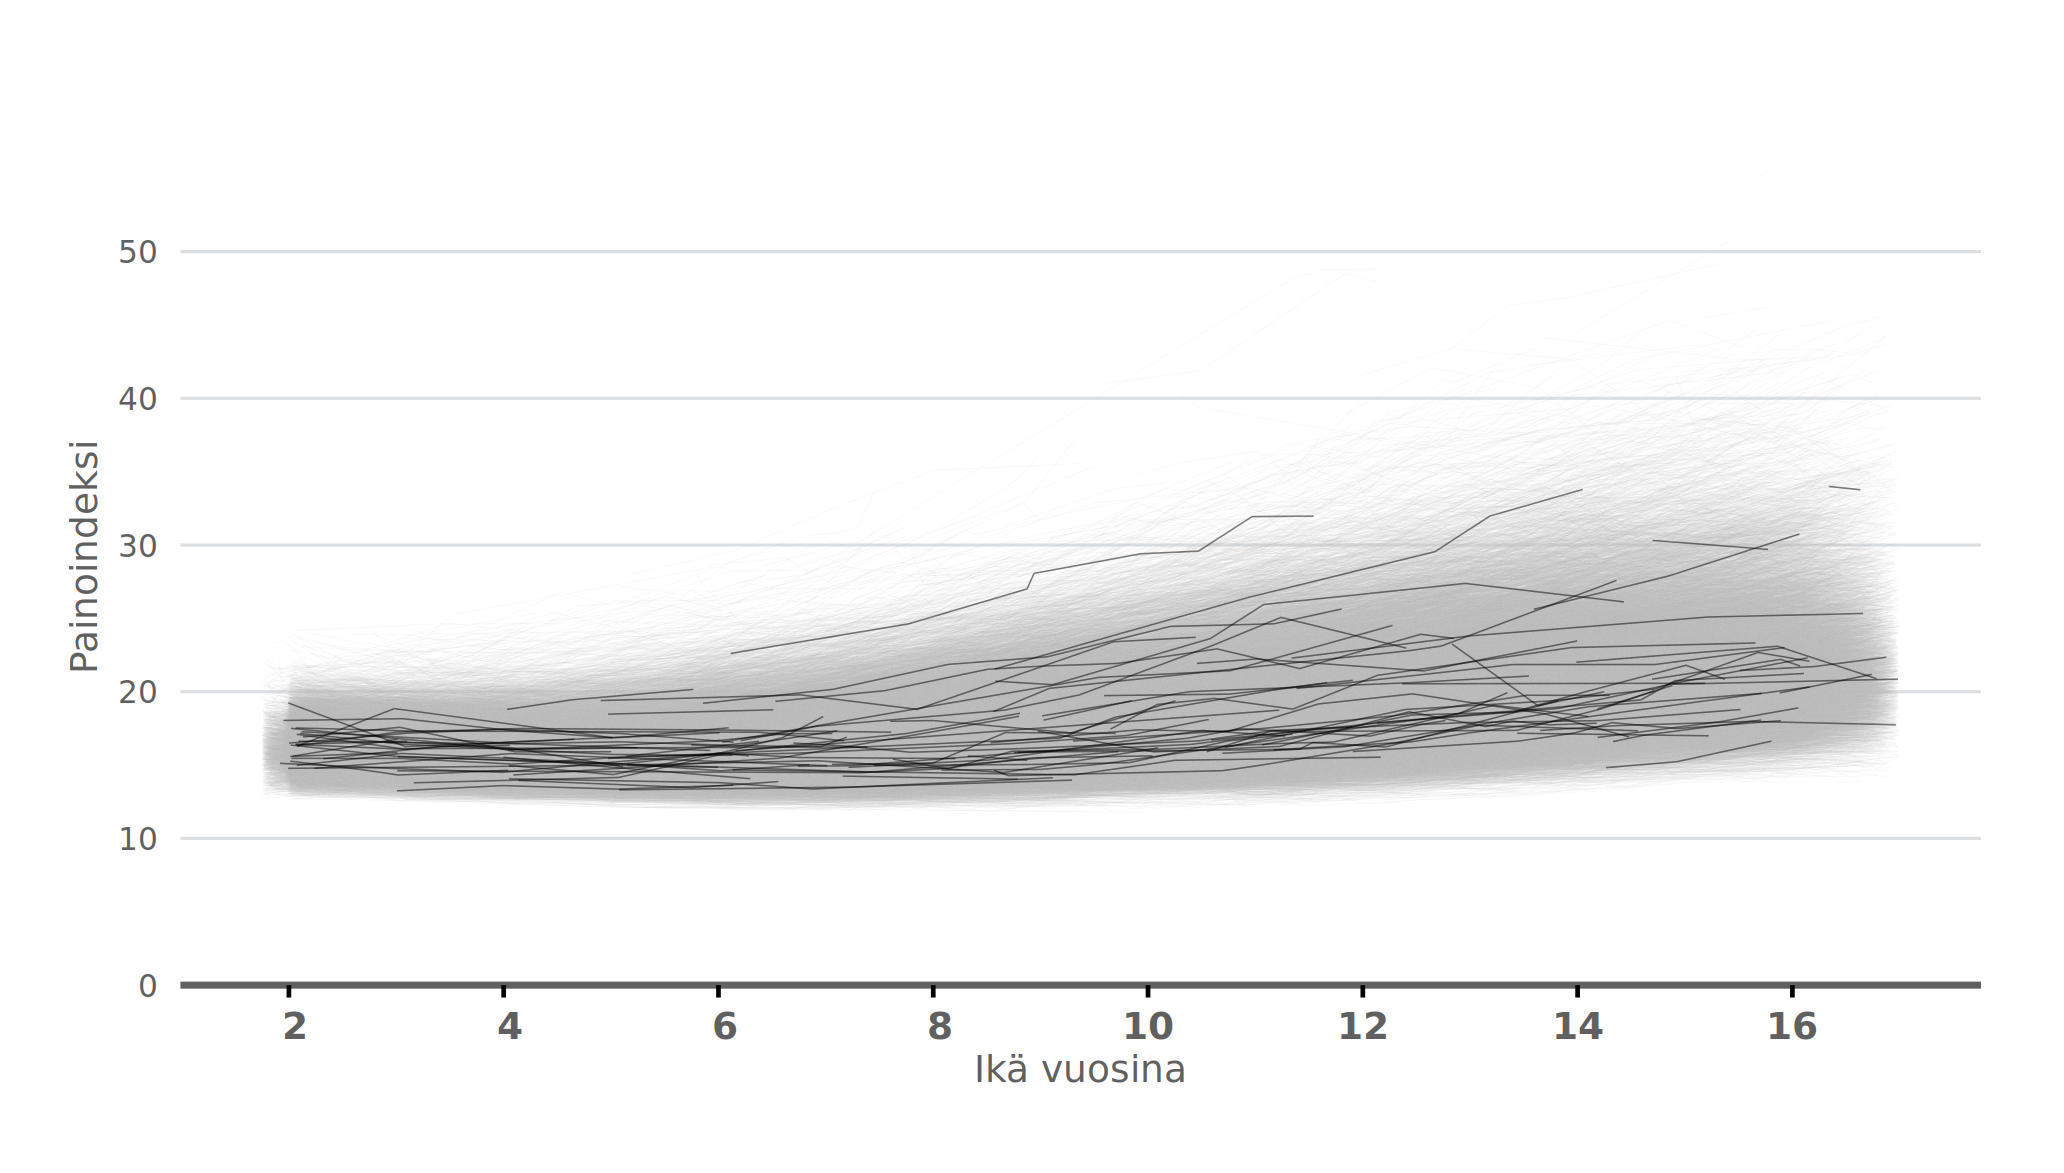
\includegraphics[scale=0.8]{kuvaajat/bmi_age.png}
  \caption{Yksilökohtaiset painoindeksiprofiilit iän mukaan (harmaa). 100 satunnaisen yksilön painoindeksiprofiilit korostettuna mustalla}
  \label{fig:bmi_age}
\end{figure}


Toinen lähde on yksilökohtainen pitkittäisvaikutus, jonka taustalla on yksilöiden vanheneminen seurannan aikana. Tästä näkökulmasta voimme vakioida ajan alkamaan ensimmäisestä mittauksesta (Kuva ~\ref{fig:bmi_follow}).\\

\begin{figure}[H]
\centering
  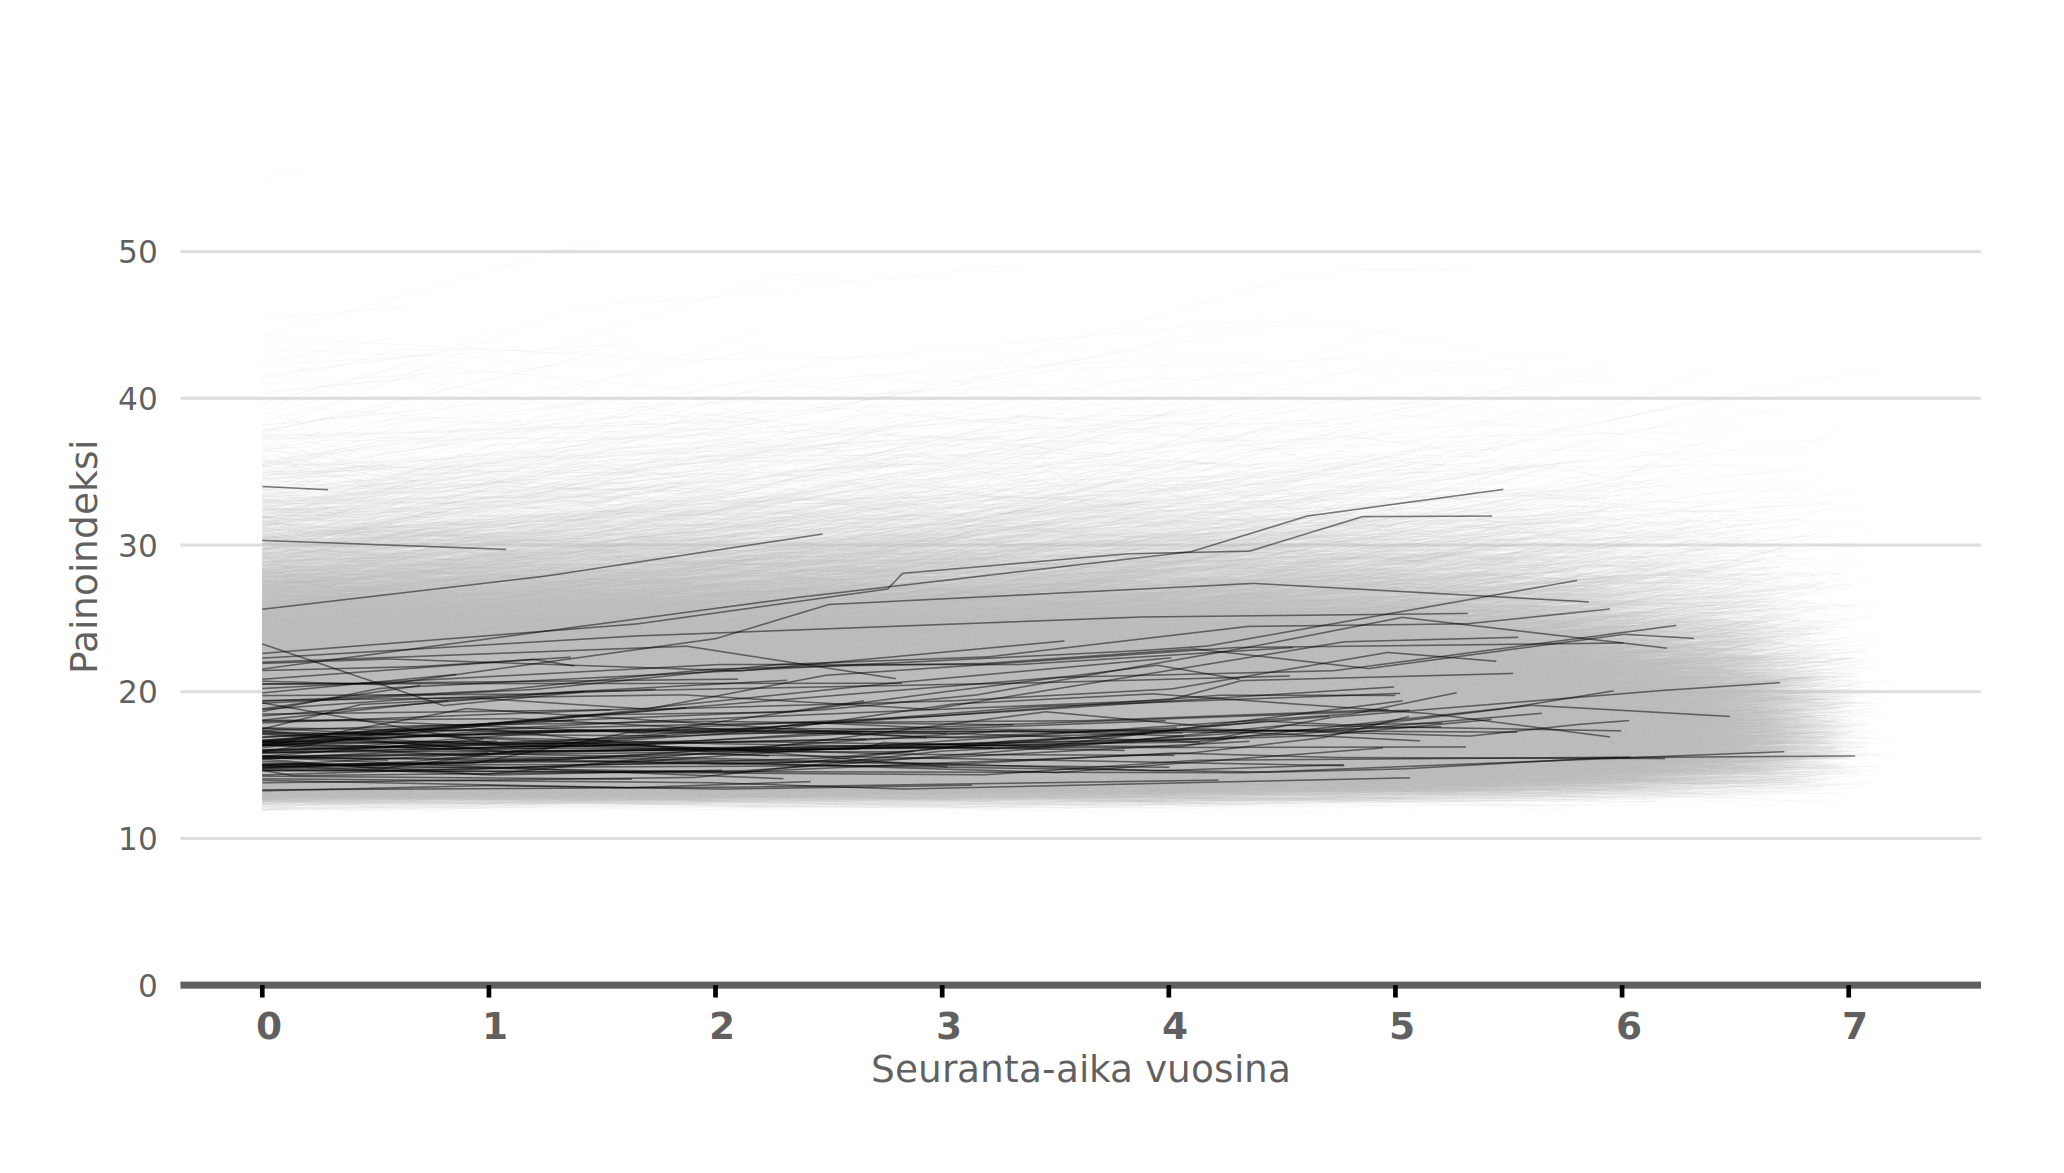
\includegraphics[scale=0.8]{kuvaajat/bmi_follow.png}
  \caption{Yksilökohtaiset painoindeksiprofiilit seuranta-ajan mukaan (harmaa). 100 satunnaisen yksilön painoindeksiprofiilit korostettuna mustalla}
  \label{fig:bmi_follow}
\end{figure}

Vaikka, koko lapsen kehityskaari huomioiden, painoindeksin kehitys voi hyvin olla epälineaarista, huomioiden vain havaitut seuranta-ajanjaksot, yksittäisen yksilön tapauksessa voimme pitää likimain kiinni lineaarisuusoletuksesta.\\

Iän mukana malliin sisällytettyjen, mahdollisesti ristiriitaisten informaation lähteiden erottamiseksi \cite{fitzmaurice11} suosittelee ajan operationalisoimista kahdeksi eri muuttujaksi, joista yksilön ikä ensimmäisellä mittauksella $\text{IKÄ}_{i0}$ (\textit{baseline age}) tuo malliin iän poikkileikkausvaikutuksen ja ikä mittaushetkellä $\text{IKÄ}_{ij}$ pitkittäisvaikutuksen. Palaamme ajan operationalisointiin mallinvalintaosiossa.\\

\subsubsection{Ylhäältä alas -strategia}
\label{ssb:ylhalas}

\cite{west14} ja \cite{verbeke00} lineaarisille sekamalleille esittämässä mallinvalintastrategiassa tavoitteena on ensin muodostaa, kiinteitä vaikutuksia lisäämäällä \textit{yliparametrisoitu} malli jolla voidaan selittää mahdollisimman hyvin aineistossa vallitsevia trendejä.\\

Toisena askeleena on löytää mallille sopiva satunnaisvaikutusten rakenne, jolla pyritään huomioimaan aineiston hierarkkinen rakenne. Tutkielman aineiston tapauksessa hierarkia syntyy ensisijaisesti satunnaisvaihtelun sallimisessa yksilökohtaisten vakiotermien ja kulmakertoimien välillä.\\

Kolmannessa vaiheessa tutkitaan satunnaisvaikutusten lisäämisen jälkeen selittämättä jäänyttä vaihtelua. Huomio kohdistuu erityisesti varianssin homoskedastisuuteen sekä yksilön mittausten väliseen autokorrelaatioon.\\ 
Viimeinen vaihe käsittää mallin parametrien kriittisen tarkastelun, varsinkin kiinteiden vaikutusten osalta ja lopullisen mallin arvioinnin.\\

Aloitamme kuitenkin tarkastelemalla painoindeksin ja iän yhteyttä, sekä lisäksi mahdollista biologisen sukupuolen vaikutusta ja iän sukupuolen yhdysvaikutusta painoindeksiin naiivissa asetelmassa lineaarisen regressiomallin avulla, sivuuttaen hetkeksi pitkittäisaineiston hierarkkisen luonteen.\\

Alustavien havaintojen (Taulukko ~\ref{table:deskrtaulu}) mukaan keskimääräinen painoindeksi kasvaa huomattavasti iän mukana, mutta sukupuolen vaikutus ilmenee monisyisempänä.\\

\begin{table}[H]
\centering
\begin{tabular}{llrrrrr}
\toprule
Sukupuoli & Ikäluokka & Keskiarvo & n & Keskihajonta & Minimi & Maksimi\\
\midrule
Poika & $[0,2)$ & 16,37 & 3113 & 1,320 & 12,92 & 23,47\\
 & $[2,7)$ & 15,98 & 80952 & 1,449 & 12,27 & 29,14\\
 & $[7,13)$ & 17,81 & 85244 & 3,186 & 12,12 & 48,81\\
 & $[13,17)$ & 20,73 & 43291 & 4,012 & 12,74 & 55,58\\
\addlinespace
Tyttö & $[0,2)$ & 16,11 & 2980 & 1,401 & 12,71 & 23,23\\
 & $[2,7)$ & 15,90 & 79334 & 1,549 & 11,93 & 30,61\\
 & $[7,13)$ & 17,73 & 84368 & 3,131 & 11,77 & 40,70\\
 & $[13,17)$ & 21,09 & 42378 & 3,729 & 12,77 & 45,55\\
\bottomrule
\end{tabular}
\caption{Painoindeksijakauman tunnuslukuja luokiteltuna biologisen sukupuolen ja ikäluokan perusteella}
\label{table:deskrtaulu}
\end{table}

Poikien keskimääräinen painoindeksi on kolmessa ensimmäisessä ikäluokassa suurempi, mutta tyttöjen painoindeksi nousee viimeisessä ikäluokassa poikien ohi. Tytöillä painoindeksin keskihajonta on poikia suurempaa kahdessa ensimmäisessä ikäluokassa, kun taas pojilla vaikuttaa olevan huomattavasti suurempi keskihajonta viimeisessä ikäluokassa. Tosin, tutkielman alussa tehdyssä jakaumatarkakastelussa havaitsimme jakaumassa vinoutta ja jakauman oikeassa hännässä merkittävästi poikkeavilla, mahdollisesti virheellisillä havainnoilla voi olla suuri vaikutus.\\

Mallin kannalta niin sukupuolen, kuin iän ja sukupuolen yhdysvaikutuksen tarkastelulle voi olla perusteita.\\

Muodostetaan ensin yksinkertainen lineaarinen regressiomalli havainnolle $i = 1,\dots, n$, jossa $n = \sum\limits_{i = 1}^{N} n_{i}$ on aineiston havaintojen kokonaismäärä


\begin{equation}
\text{BMI}_i = \beta_0 + \beta_1 \times \text{IKÄ}_i + \epsilon_i \label{eq:lm1}\\
\end{equation}


Regressiokertoimen $\beta_0$ estimaatiksi (Taulukko ~\ref{table:lm1}) saamme likimain 13,94. Tämä niin kutsuttu vakiotermi voidaan tulkita keskimääräiseksi painoindeksiksi, kun muuttuja $\text{IKÄ}_i$ saa arvon 0. Itse estimaatin arvo ei siis itsessään ole kovin mielekäs, sillä aineston havainnot alkavan noin kahdesta ikävuodesta. Tarvittaessa tilanne voitaisi korjata skaalaamalla ikämuuttujaa siirtäen vakiotermin estimaatin vastaamaan haluttua ikää.\\

\begin{table}[H]
\centering
\begin{tabular}{llllll}
\toprule
  & Estimaatti & Keskivirhe ($\text{se}$) & P & $\text{LV}_{2,5}$ & $\text{LV}_{97,5}$\\
\midrule
$\hat{\beta}_0$ & 13,939 & 0,0098 & 0,0000 & 13,920 & 13,958\\
$\hat{\beta}_1$ & 0,4310 & 0,0010 & 0,0000 & 0,4291 & 0,4330\\
\bottomrule
\end{tabular}
\caption{Yksinkertaisen lineaarisen regressiomallin ~\ref{eq:lm1} parametrien estimaatit ja keskivirheet}
\label{table:lm1}
\end{table}

Regressiokertoimen $\beta_1$ estimaatti 0,4310, voidaan tulkita puolestaan PNS-menetelmällä sovitetun regressiosuoran kulmakertoimeksi. Toisin sanoen jokaista ikävuoden yksikkömuutosta kohden keskimääräinen painoindeksi kasvaa likimain 0,43 yksikköä.\\

Huomioitavaa on, että yksinkertaisen regressiomallin parametrien keskivirheen määritelmästä

$$
se(\hat{\beta}_0)= \sqrt{\hat{\sigma}^2 \Bigg( \frac{1}{n}+\frac{( \frac{1}{n}\sum\limits_{i = 1}^{n}\text{IKÄ}_i)^2}{\sum_{i=1}^n (\text{IKÄ}_i- \frac{1}{n}\sum\limits_{i = 1}^{n}\text{IKÄ}_i)^2} \Bigg)}\,\!
$$

$$
\text{se}(\hat{\beta}_1) = \sqrt{\frac{\hat{\sigma}^2}{\sum_i (\text{IKÄ}_i - \frac{1}{n}\sum\limits_{i = 1}^{n}\text{IKÄ}_i)^2}}
$$

, jossa $\hat{\sigma}^2 = \frac{1}{n-2} \sum_i \hat{\epsilon}_i^2$,\\

seuraa, että havaintomäärän $n$ ollessa hyvin suuri keskivirheet jäävät aina pieniksi. Teknisessä mielessä, voimme siis luottaa, että estimaattorimme tuottamat estimaatit ovat täsmällisiä, mutta ne voivat silti olla hyvinkin harhaisia.\\

Tutkitaan seuraavaksi sukupuolen vaikutusta lisäämällä malliin muuttuja $\text{SUKUPUOLI}_i$\\

\begin{equation}
\text{BMI}_i = \beta_0 + \beta_1 \times \text{IKÄ}_i + \beta_2 \times \text{SUKUPUOLI}_i + \epsilon_i \label{eq:lm2}\\
\end{equation}

Vaikuttaisi siltä, että sukupuolella ei vaikuttaisi olevan merkitsevää vaikutusta keskimääräiseen painoindeksiin (Taulukko ~\ref{table:lm2}). Tässä tapauksessa tilastollinen merkitsevyys $\text{P}$ päätellään vertaamaalla T-testisuureen arvoa $t_0$ $t$-jakauman arvoon $T$.\\

\begin{table}[H]
\centering
\begin{tabular}{llllll}
\toprule
  & Estimaatti & Keskivirhe ($\text{se}$) & P & $\text{LV}_{2,5}$ & $\text{LV}_{97,5}$\\
\midrule
$\hat{\beta}_0$ & 13,940 & 0,0107 & 0,0000 & 13,919 & 13,961\\
$\hat{\beta}_1$ & 0,4310 & 0,0010 & 0,0000 & 0,4291 & 0,4330\\
$\hat{\beta}_2$ & -0,0025 & 0,0086 & 0,7761 & -0,0194 & 0,0145\\
\bottomrule
\end{tabular}
\caption{Lineaarisen regressiomallin ~\ref{eq:lm2} parametrien estimaatit ja keskivirheet kun malliin on lisätty biologisen sukupuolen vaikutus}
\label{table:lm2}
\end{table}

Testisuure

$$
t_0 = \frac{\hat{\beta}_2 - 0}{\text{se}(\hat{\beta}_2)},
$$

noudattaa $t$-jakaumaa vapausastein $n-2$, jolloin P-arvoksi saadaan

$$
\text{P} = 2(1-P(T \leq t_0)).
$$

P-arvo tiivistää informaatiota siitä, kuinka kaukana estimaatti $\hat{\beta}_2$ on nollasta suhteessa estimaattorin täsmällisyyteen.\\

Tarkastellaan kolmatta mallia, jossa lisäämme iän ja sukupuolen yhdysvaikutuksen.\\

\begin{equation}
\text{BMI}_i = \beta_0 + \beta_1 \times \text{IKÄ}_i + \beta_2 \times \text{SUKUPUOLI}_i + \beta_3 \times \text{IKÄ}_i \times \text{SUKUPUOLI}_i + \epsilon_i \label{eq:lm3}\\
\end{equation}

Nyt sekä sukupuoli, että iän ja sukupuolen yhdysvaikutukset ovat merkitseviä. Mallin tuloksista (~\ref{table:lm3}) voimme nähdä, että iän estimaatti on hieman edellistä pienempi. Nyt iän estimaatti viittaa päävaikutukseen, kun sukupuolena on poika, kun taas iän ja sukupuolen yhdysvaikutus viittaa muutokseen iän päävaikutuksesta, kun sukupuolena tyttö.\\

\begin{table}[H]
\centering
\begin{tabular}{llllll}
\toprule
  & Estimaatti & Keskivirhe ($\text{se}$) & P & $\text{LV}_{2,5}$ & $\text{LV}_{97,5}$\\
\midrule
$\hat{\beta}_0$ & 14,079 & 0,0138 & 0,0000 & 14,052 & 14,1060\\
$\hat{\beta}_1$ & 0,4151 & 0,0014 & 0,0000 & 0,4123 & 0,4179\\
$\hat{\beta}_2$ & -0,2831 & 0,0196 & 0,0000 & -0,3215 & -0,2447\\
$\hat{\beta}_3$ & 0,0322 & 0,0020 & 0,0000 & 0,0283 & 0,0362\\
\bottomrule
\end{tabular}
\caption{Lineaarisen regressiomallin ~\ref{eq:lm3} parametrien estimaatit ja keskivirheet kun malliin on lisätty biologisen sukupuolen ja iän yhdysvaikutus}
\label{table:lm3}
\end{table}

\begin{figure}[H]
\centering
  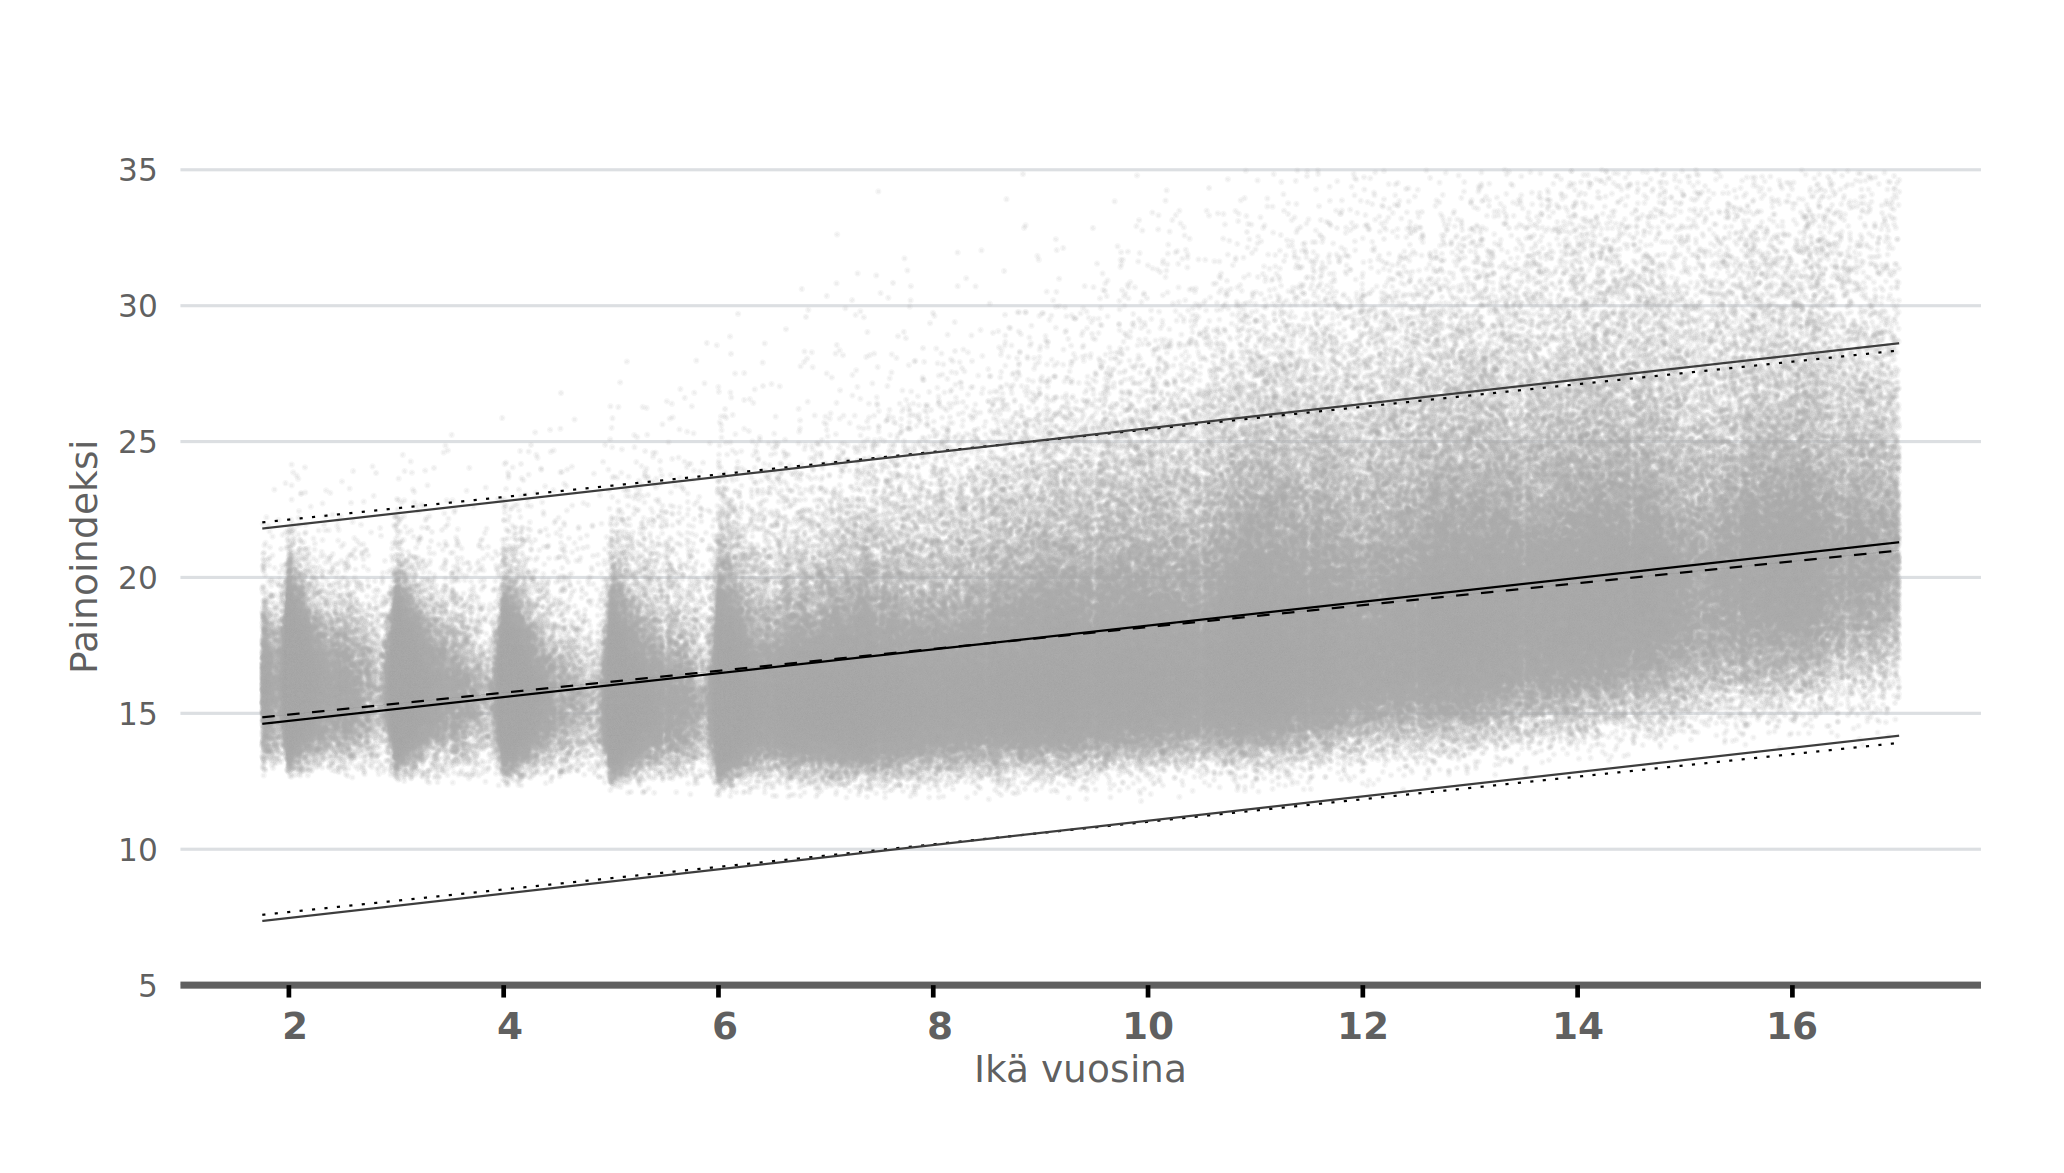
\includegraphics[scale=0.8]{kuvaajat/lm_baseline.png}
  \caption{Riippumattomiin mittauksiin sovitettu lineaarinen malli iän ja sukupuolen yhdysvaikutus huomioituna ennusteväleineen. Tytöt yhtenäisillä viivoilla, pojat katkoviivalla.}
  \label{fig:lm_baseline}
\end{figure}

Iän ja sukupuolen yhdysvaikutus vaikuttaa kuitenkin melko pieneltä ja sovitteen sekä aineiston visuaalinen tarkastelu (Kuva ~\ref{fig:lm_baseline}) viittaa samaan. Lisäksi on selvää, että kyseinen malli on hyvin puuttellinen tämän kaltaiseen aineistoon. Jo visuaalinen tarkastelu paljastaa, että naiivissa asetelmassa mallin oletukset lineaarisuudesta, residuaalien normaalisuudesta ja varianssin homoskedastisuudesta eivät täyty.\\

On kuitenkin muistettava, että tavoitteenamme on muodostaa yliparametrisoitu kiinteiden vaikutusten malli ja teemme varsinaisen kriittisen mallinvalinnan myöhemmässä vaiheessa.\\

Edellä sovitettujen mallien vertailu (Taulukko ~\ref{table:lm_summary}) osoittaa, että pelkän sukupuolen lisäämisellä malliin ei ole suotuisaa vaikutusta, mutta iän ja sukupuolen yhdysvaikutus parantaa mallin yhteensopivuutta maltillisesti. 

\begin{table}[H]
\centering
\begin{tabular}{lrrrr}
\toprule
Malli & $df$ & $l(\bm{\beta})$ & AIC & BIC\\
\midrule
LM ~\ref{eq:lm1} & 3 & -1033025 & 2066056 & 2066089\\
LM ~\ref{eq:lm2} & 4 & -1033025 & 2066058 & 2066102\\
LM ~\ref{eq:lm3} & 5 & -1032898 & 2065806 & 2065861\\
\bottomrule
\end{tabular}
\caption{Lineaaristen mallien vapausasteiden, log-uskottavuuksien ja informaatiokriteerien vertailu}
\label{table:lm_summary}
\end{table}

Bayesin informaatiokriteeri, erityisesti mallien LM ~\ref{eq:lm1} ja LM ~\ref{eq:lm3} välillä, näyttää, että parametrien ja havaintojen määrä huomioiden malli on vain hieman paremmin sopusoinnussa aineiston kanssa.\\

Yliparametrisoidun kiinteiden vaikutusten mallin tarpeet täyttääksemme, voimme silti ottaa lineaarisen mallin LM ~\ref{eq:lm3}.\\

\subsubsection{Yliparametrisoitu kiinteiden vaikutusten malli}
\label{ssb:yliparammalli}

Siirrämme lähestymistavan nyt pitkittäisaineiston kehikkoon. Muotoilemme kiinteiden vaikutusten mallin, noudattaen \cite{fitzmaurice11} suositusta ajan operationalisoinnista, seuraavalla tavalla

\begin{equation}
\begin{split}
 \text{BMI}_{ij} = \beta_0 + \beta_1 \times \text{IKÄ}_{i0} + \beta_2 \times \text{IKÄ}_{ij} + \beta_3 \times \text{SUKUPUOLI}_{ij}  \\
 + \beta_4 \times \text{IKÄ}_{ij} \times \text{SUKUPUOLI}_{ij} + \text{b}_{0i} + \epsilon_{ij}
\label{eq:lme1}
\end{split}
\end{equation}

\cite{west14} kuvaa kiinteiden vaikutusten mallia keskiarvorakenteeksi (\textit{mean structure}), sillä se pyrkii kuvaamaan lineaarisen regression tavoin keskimääräistä yhteyttä vastemuuttujan ja taustamuuttujien välillä.

Kiinteiden vaikutusten ML-estimaateilla (Taulukko ~\ref{table:lme0}) onkin vastaava tulkinta kuin lineaarisen regressiomallin (Taulukko ~\ref{eq:lm3}) estimaateilla. Huomaamme, että estimaatit vastaavat likimain toisiaan, joskin aikadimension uudelleenoperationalisointi on lisännyt malliin uuden parametrin.\\

\begin{table}[H]
\centering
\begin{tabular}{llllll}
\toprule
  & Estimaatti & Keskivirhe ($\text{se}$) & P & $\text{LV}_{2,5}$ & $\text{LV}_{97,5}$\\
\midrule
$\hat{\beta}_0$ & 14,124 & 0,0189 & 0,0000 & 14,087 & 14,161\\
$\hat{\beta}_1$ & 0,0194 & 0,0022 & 0,0000 & 0,0152 & 0,0236\\
$\hat{\beta}_2$ & 0,4044 & 0,0015 & 0,0000 & 0,4016 & 0,4073\\
$\hat{\beta}_3$ & -0,3285 & 0,0231 & 0,0000 & -0,3737 & -0,2833\\
$\hat{\beta}_4$ & 0,0404 & 0,0019 & 0,0000 & 0,0367 & 0,0442\\
\bottomrule
\end{tabular}
\caption{Keskiarvorakenteen kiinteiden vaikustusten ML-estimaatit}
\label{table:lme0}
\end{table}

Keskeinen ero on kuitenkin yksilöiden välinen satunnaisvaikutus $b_{i0}$, joka kiinteiden vaikutusten mallissa kuvaa yksilöiden vakiotermin vaihtelua. \\

Koska $\bm{b}_i \sim N(0,\bm{G})$, ainoastaan vakiotermin vaihtelun sisältävän mallimme satunnaisvaikutusten kovarianssimatriisi on siten

$$
\bm{G} = 
\begin{bmatrix}
\text{Var}({\text{b}_{0i}})\\
\end{bmatrix} =
\begin{bmatrix}
\sigma^2_{\text{b}_{0i}}\\
\end{bmatrix}.
$$

Oletamme vielä toistaiseksi residuaalit $\bm{\epsilon}_i \sim N(0, \bm{R}_i)$ korreloimattomiksi, jolloin matriisilla $\bm{R}_i$ on diagonaalirakenne

$$
\bm{R}_i =
\begin{bmatrix}
\sigma^2 & \dots & 0 \\
\vdots & \ddots & \vdots \\
0 & \dots & \sigma^2 \\
\end{bmatrix}.
$$

Estimaateista $\hat{\bm{G}}$ ja $\hat{\bm{R}}_i$ (Taulukko ~\ref{table:lme1}) saamme alustavia, joskaan ei yllättäviä viitteitä, että yksilöiden keskimääräisten painoindeksien varianssi on suurempaa, kuin yksilökohtaisten residuaalien varianssi.\\

\begin{table}[H]
\centering
\begin{tabular}{llllll}
\toprule
  & Estimaatti & Keskivirhe ($\text{se}$) & P & $\text{LV}_{2,5}$ & $\text{LV}_{97,5}$\\
\midrule
$\hat{\sigma^2}_{\text{b}_{0i}}$ & 6,224 & 2,495 & 0 & 6,167* & 6,280*\\
\addlinespace
$\hat{\sigma^2}$ & 1,382 & 1,176 & 0 & 1,376* & 1,387*\\
\bottomrule
\end{tabular}
\caption{Keskiarvorakenteen satunnaisvaikustusten ja residuaalien varianssi-kovarianssiestimaatit. *Luottamusvälit arvioitu normaaliapproksimaatiolla (\cite{pinheiro00})}
\label{table:lme1}
\end{table}

Kiinteiden vaikutusten mallin lähtöaineistolle ennustetuista arvoista (Kuva ~\ref{fig:lme1_bmi_pred}) vahvistamme vakiotermin satunnaisvaikutusten intuitiivisen tulkinnan. Yksilöillä on sama \textit{keskiarvorakenne}, mutta vakiotermit vaihtelevat.\\

\begin{figure}[H]
\centering
  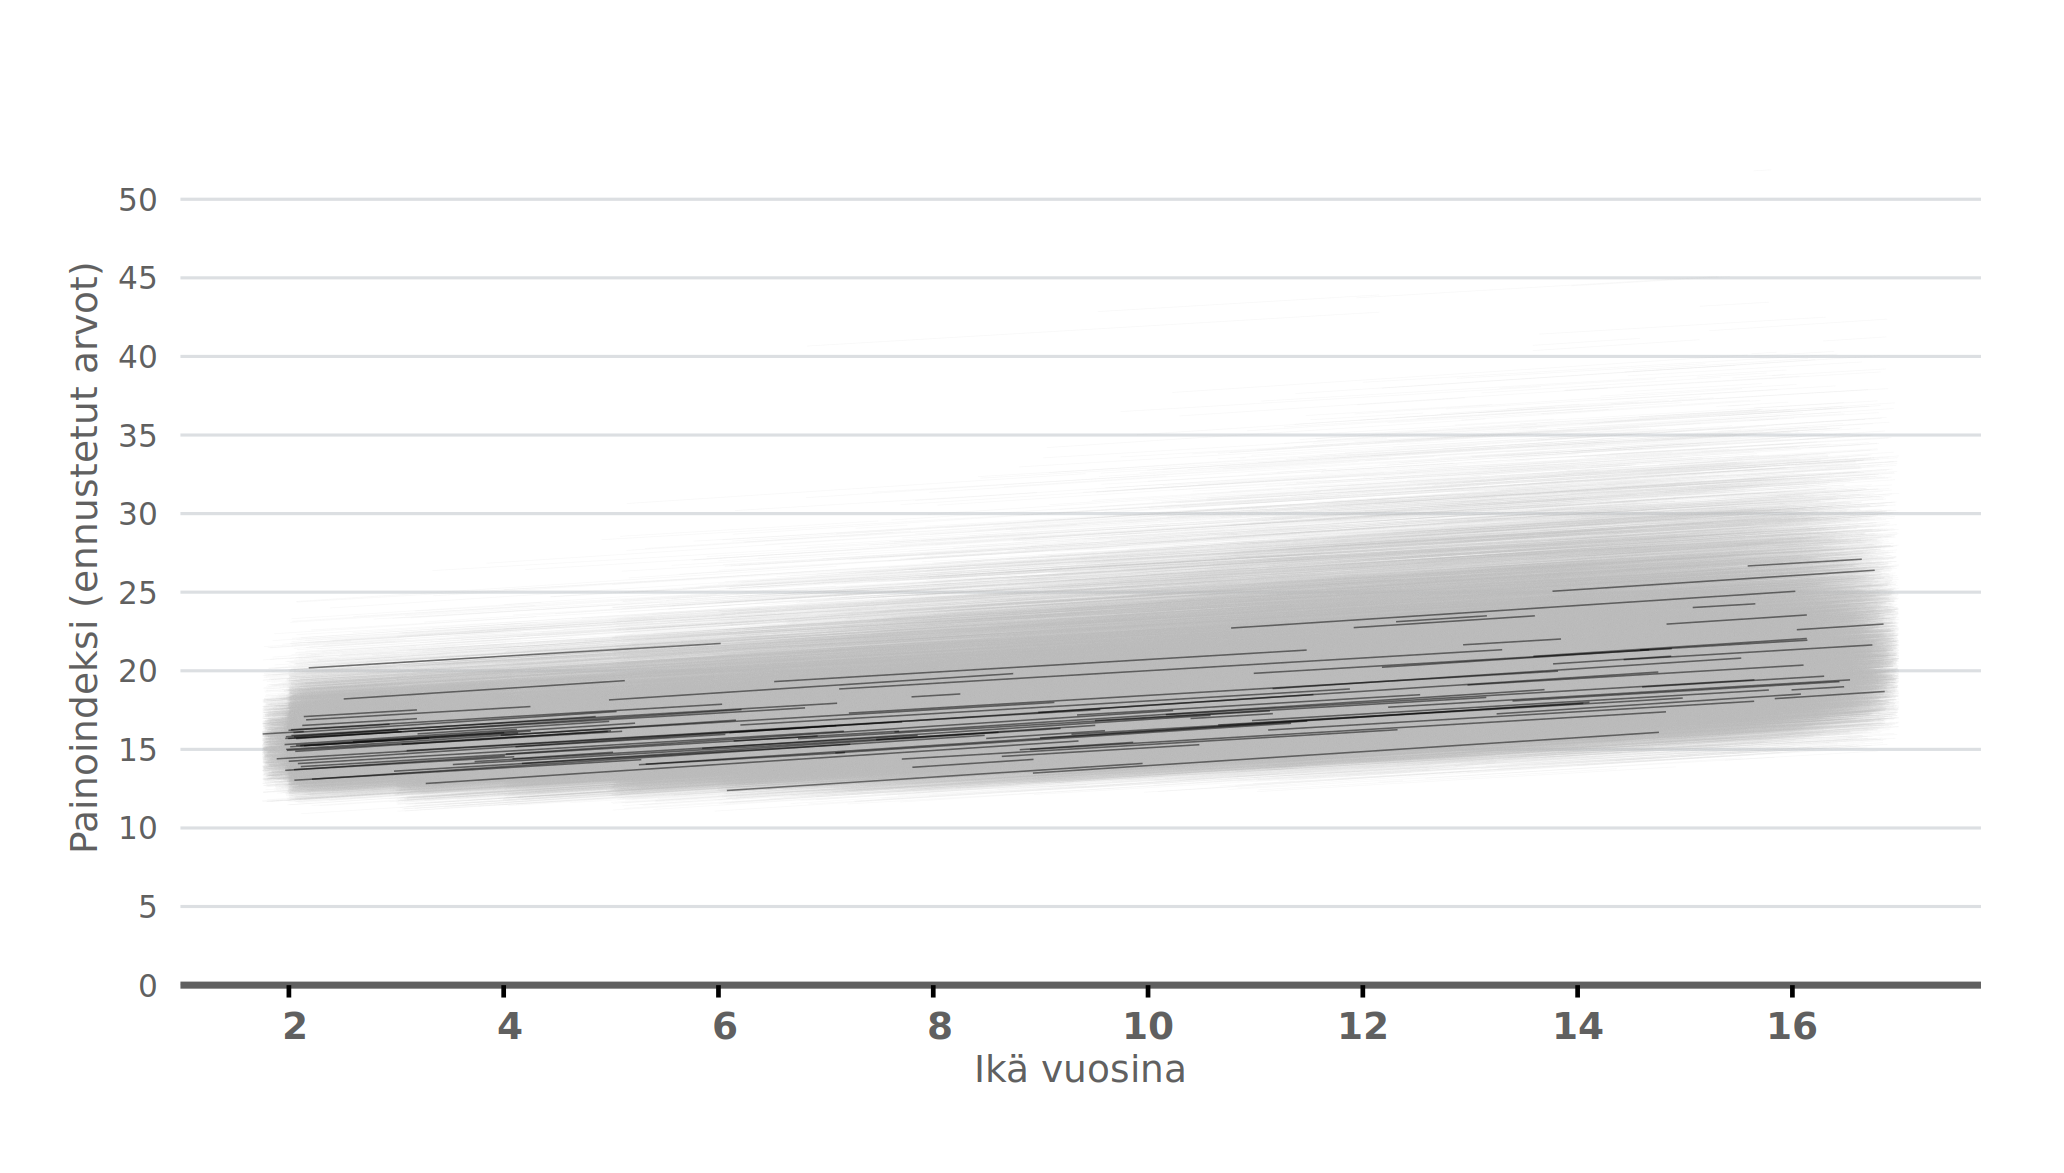
\includegraphics[scale=0.8]{kuvaajat/lme_bmi_ennuste.png}
  \caption{Kiinteiden vaikutusten mallin lähtöaineistolle ennustetut painoindeksin arvot. Sadan satunnaisen yksilön profiilit korostettuna mustalla.}
  \label{fig:lme1_bmi_pred}
\end{figure}

Vakiotermin satunnaisvaikutusten $\text{b}_{0i}$ (Kuva ~\ref{fig:lme1_ranef}) ja yksilökohtaisten residuaalien $\bm{\epsilon}_i$ (Kuva ~\ref{fig:lme1_resid}) jakaumien tarkastelu paljastavat ongelmia molempien jakaumaoletuksissa. $\text{b}_{0i}$ jakaumassa on havaittavissa vinoutta ja $\bm{\epsilon}_i$ jakaumassa ilmenee alaspäin suuntautuvaa harhaa.\\

\begin{figure}[H]
\centering
  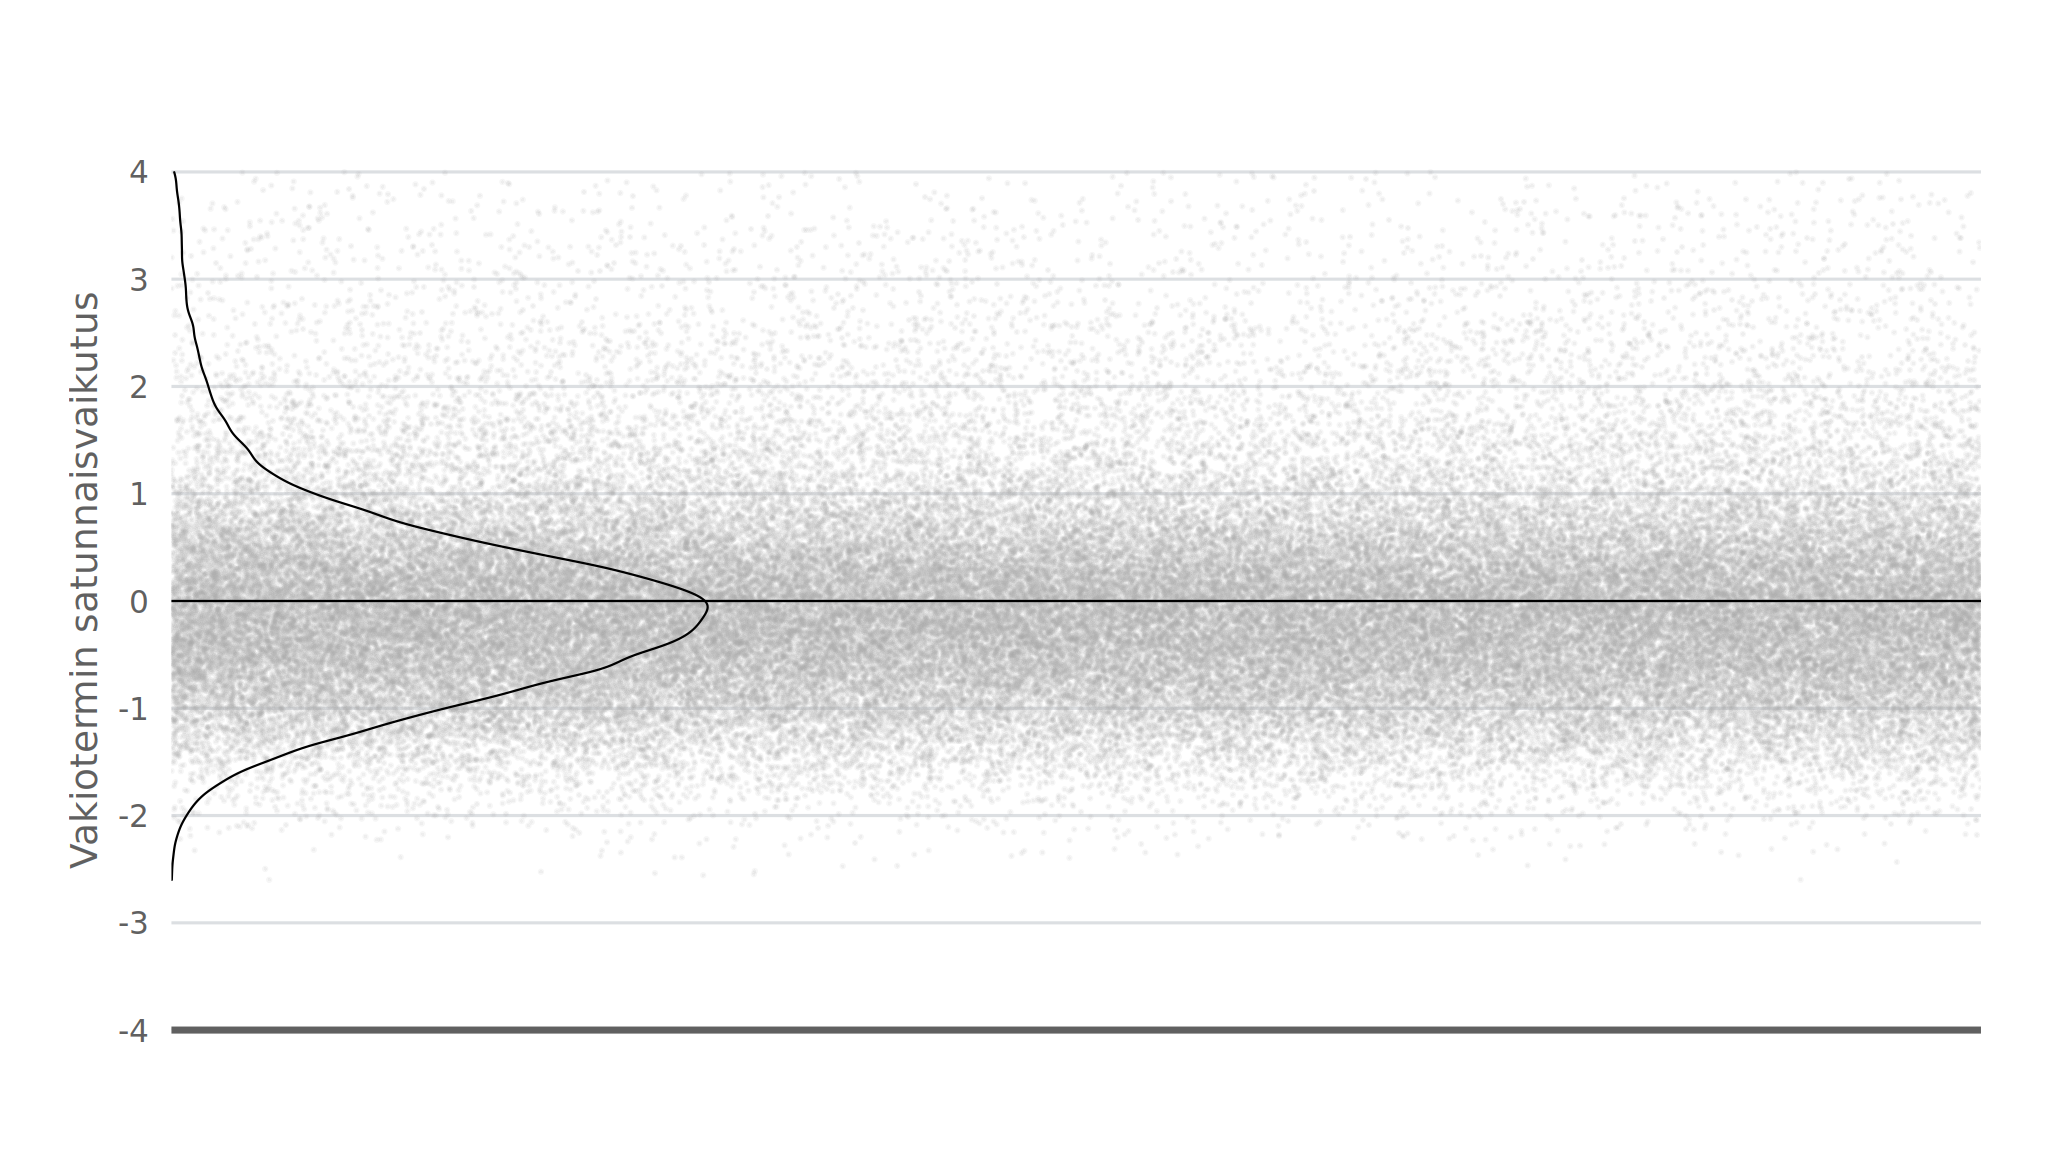
\includegraphics[scale=0.8]{kuvaajat/lme_satunnaisvaikutukset.png}
  \caption{Kiinteiden vaikutusten mallin vakiotermin ennustetut satunnaisvaikutukset ja tiheysfunktion Gaussin ydinestimaatti}
  \label{fig:lme1_ranef}
\end{figure}

\begin{figure}[H]
\centering
  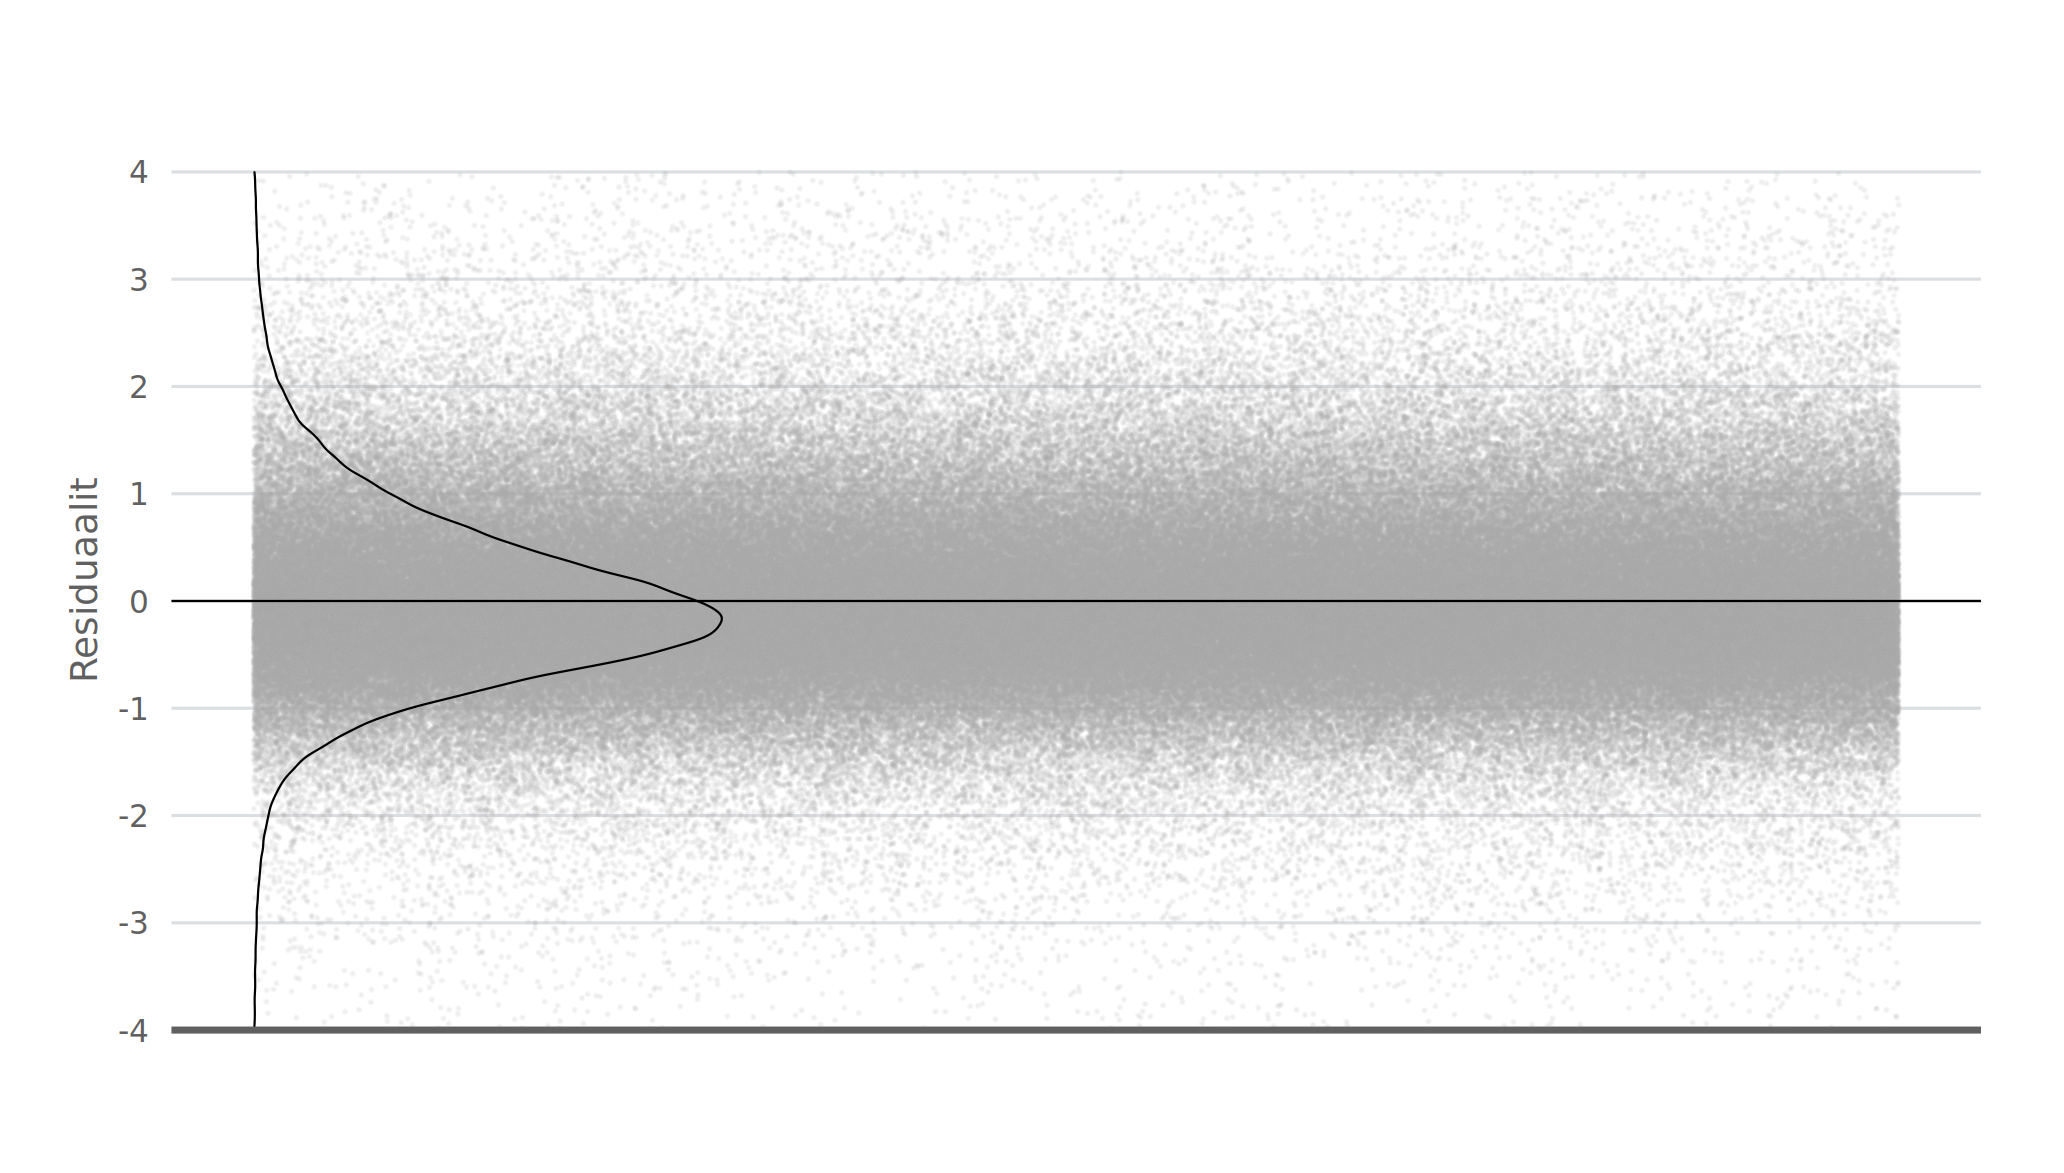
\includegraphics[scale=0.8]{kuvaajat/lme_residuaalit.png}
  \caption{Kiinteiden vaikutusten mallin yksilökohtaisten mittausten Pearson-residuaalit ja tiheysfunktion Gaussin ydinestimaatti}
  \label{fig:lme1_resid}
\end{figure}

Kiinteiden vaikutusten malli ei sellaisenaan vaikuta riittävältä tutkielman aineiston analyysivälineeksi. Tarkastellaan, kuinka satunnaisvaikutusten rakennetta tarkentamalla voisimme parantaa mallin yhteensopivuutta.\\

\subsubsection{Satunnaisvaikutusten rakenteen valinta}
\label{ssb:satunnaisrakenneval}

Aineiston tarkastelun perustella (Kuva \ref{fig:bmi_age}) on uskottavaa ajatella, että painoindeksin ja iän suhteessa, keskimääräisten erojen lisäksi myös kehityksessä iän suhteen olisi yksilöiden välillä eroa. \\

Tutkimme seuraavaksi millainen seuraus iän satunnaisvaikutuksen lisäämisellä on malliin. Kirjoitetaan malli yksilön $i$ painoindeksihavainnolle $j$

\begin{equation}
\begin{split}
 \text{BMI}_{ij} = \beta_0 + \beta_1 \times \text{IKÄ}_{i0} + \beta_2 \times \text{IKÄ}_{ij} + \beta_3 \times \text{SUKUPUOLI}_{ij} \\
+ \beta_4 \times \text{IKÄ}_{ij} \times \text{SUKUPUOLI}_{ij} + \text{b}_{0i} + \text{b}_{1i} \times \text{IKÄ}_{ij} + \epsilon_{ij},
\label{eq:lme2}
\end{split}
\end{equation}

jossa $\text{b}_{i0}$ vakiotermin satunnaisvaikutus ja $\text{b}_{i1}$ iän satunnaisvaikutus.\\ 

Merkitään satunnaisvaikutusten parametrivektoria

$$
\bm{b}_i =
\begin{bmatrix}
\text{b}_{i0} \\
\text{b}_{i1} \\
\end{bmatrix},
$$

jolloin kovarianssimatriisi $\bm{G}$ on

$$
\bm{G} =
\begin{bmatrix}
\text{Var}(\text{b}_{0i}) & \text{Cov}(\text{b}_{0i}, \text{b}_{1i}) \\
\text{Cov}(\text{b}_{0i}, \text{b}_{1i}) & \text{Var}(\text{b}_{1i}) \\
\end{bmatrix} =
\begin{bmatrix}
\sigma^2_{\text{b}_{0i}} & \sigma_{\text{b}_{0i}, \text{b}_{1i}} \\
\sigma_{\text{b}_{0i}, \text{b}_{1i}} & \sigma^2_{\text{b}_{1i}} \\
\end{bmatrix}.
$$

Matriisille $\bm{R}_i$ oletamme edelleen korreloimattoman diagonaalirakenteen.\\

Satunnaisvaikutuksia vertallaksemme sovitamme mallin REML-menetelmällä. Koska kiinteiden vaikutusten ja satunnaisvaikutusten mallien kiinteät vaikutukset ovat samoin määritelty, voidaan aiemmin ML-menetelmällä estimoituja kiinteitä vaikutuksia (Taulukko ~\ref{table:lme0}) kuitenkin verrata satunnaisvaikutusten REML-estimaatteihin (Taulukko ~\ref{table:lme2}).

\begin{table}[H]
\centering
\begin{tabular}{llllll}
\toprule
  & Estimaatti & Keskivirhe ($\text{se}$) & P & $\text{LV}_{2,5}$ & $\text{LV}_{97,5}$\\
\midrule
$\hat{\beta}_0$ & 14,616 & 0,0175 & 0,0000 & 14,582 & 14,651\\
$\hat{\beta}_1$ & -0,1722 & 0,0020 & 0,0000 & -0,1762 & -0,1682\\
$\hat{\beta}_2$ & 0,3832 & 0,0024 & 0,0000 & 0,3784 & 0,3879\\
$\hat{\beta}_3$ & -0,3614 & 0,0225 & 0,0000 & -0,4055 & -0,3173\\
$\hat{\beta}_4$ & 0,0432 & 0,0034 & 0,0000 & 0,0366 & 0,0497\\
\bottomrule
\end{tabular}
\caption{Satunnaisvaikutusten mallin LSM~\ref{eq:lme2} kiinteiden vaikustusten REML-estimaatit}
\label{table:lme2}
\end{table}

Taulukosta ~\ref{table:lme3} huomaamme vakiotermin varianssin kasvaneen hieman, mutta toisaalta residuaalivarianssi on pienentynyt huomattavasti. Malli vaikuttaa siis selittävän yksilökohtaisten mittausten vaihtelua paremmin.\\

\begin{table}[H]
\centering
\begin{tabular}{llllll}
\toprule
  & Estimaatti & Keskivirhe ($\text{se}$) & P & $\text{LV}_{2,5}$ & $\text{LV}_{97,5}$\\
\midrule
$\hat{\sigma^2}_{\text{b}_{0i}}$ & 8,4467 & 2,9063 & 0 & 8,2955* & 8,6007*\\
$\hat{\sigma^2}_{\text{b}_{1i}}$ & 0,2116 & 0,4600 & 0 & 0,2091* & 0,21413*\\
$\hat{\sigma}_{\text{b}_{0i}, \text{b}_{1i}}$ & -1,0566 & - & - & - & -\\
\addlinespace
$\hat{\sigma^2}$ & 0,5926 & 1,176 & 0 & 0,5889* & 0,5964*\\
\bottomrule
\end{tabular}
\caption{Satunnaisvaikutusmallin LSM~\ref{eq:lme2} satunnaisvaikustusten ja residuaalien varianssi-kovarianssiestimaatit. Kovarianssille ei saatavilla keskivirhettä tai luottamusvälejä (-). *Luottamusvälit arvioitu normaaliapproksimaatiolla (\cite{pinheiro00})}
\label{table:lme3}
\end{table}

Aineistolle ennustettujen painoindeksiarvojen tarkastelu (Kuva ~\ref{fig:lme2_bmi_pred}) viittaa samankaltaiseen johtopäätökseen. Yksilöiden mittausjaksot vaiktutavat eroavan toisistaan iästä riippuen. Nuoremmilla lapsilla kehityksen vaihtelu on maltillisempaa, mutta vanhemmilla lapsilla ja nuorilla painoindeksin kehitys vaihtelee iän satunnaisvaikutuksien perusteellaa huomattavasti enemmän.\\

\begin{figure}[H]
\centering
  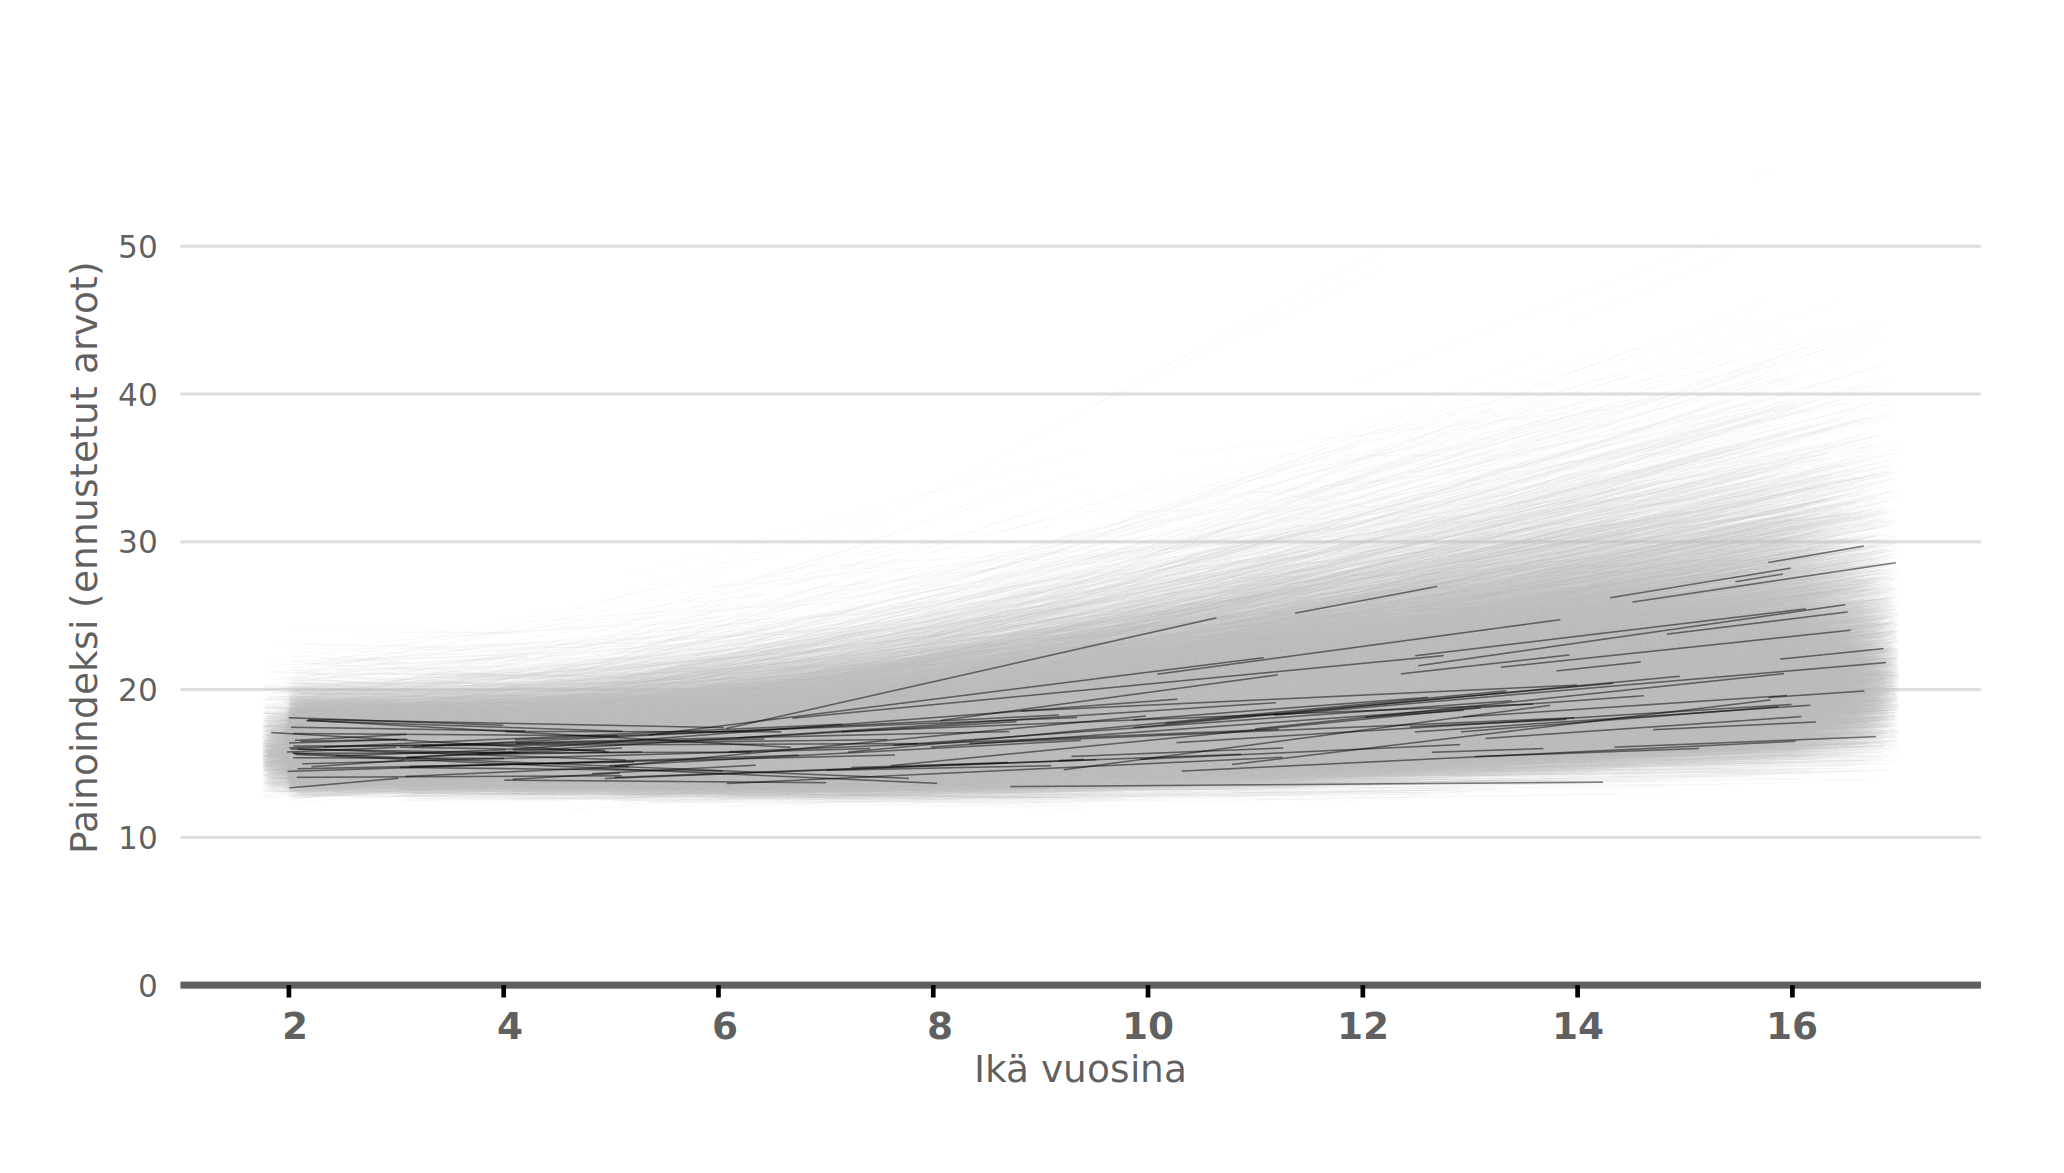
\includegraphics[scale=0.8]{kuvaajat/lme2_bmi_ennuste.png}
  \caption{Satunnaisvaikutusten mallin LSM~\ref{eq:lme2} lähtöaineistolle ennustetut painoindeksin arvot. Sadan satunnaisen yksilön profiilit korostettuna mustalla.}
  \label{fig:lme2_bmi_pred}
\end{figure}

Vakiotermin ennustettujen satunnaisvaikutusten jakauma (Taulukko ~\ref{fig:lme2_vakio_ranef}) on silmämääräisesti symmetrisempi kuin kiinteiden vaikutusten mallissa, mutta iän ennustetuissa satunnaisvaikutukset (Taulukko ~\ref{fig:lme2_ika_ranef}) ovat mahdollisesti harhaisia. Paneudumme tähän lopullisen mallin kriittisessä arvioinnissa.\\

\begin{figure}[H]
\centering
  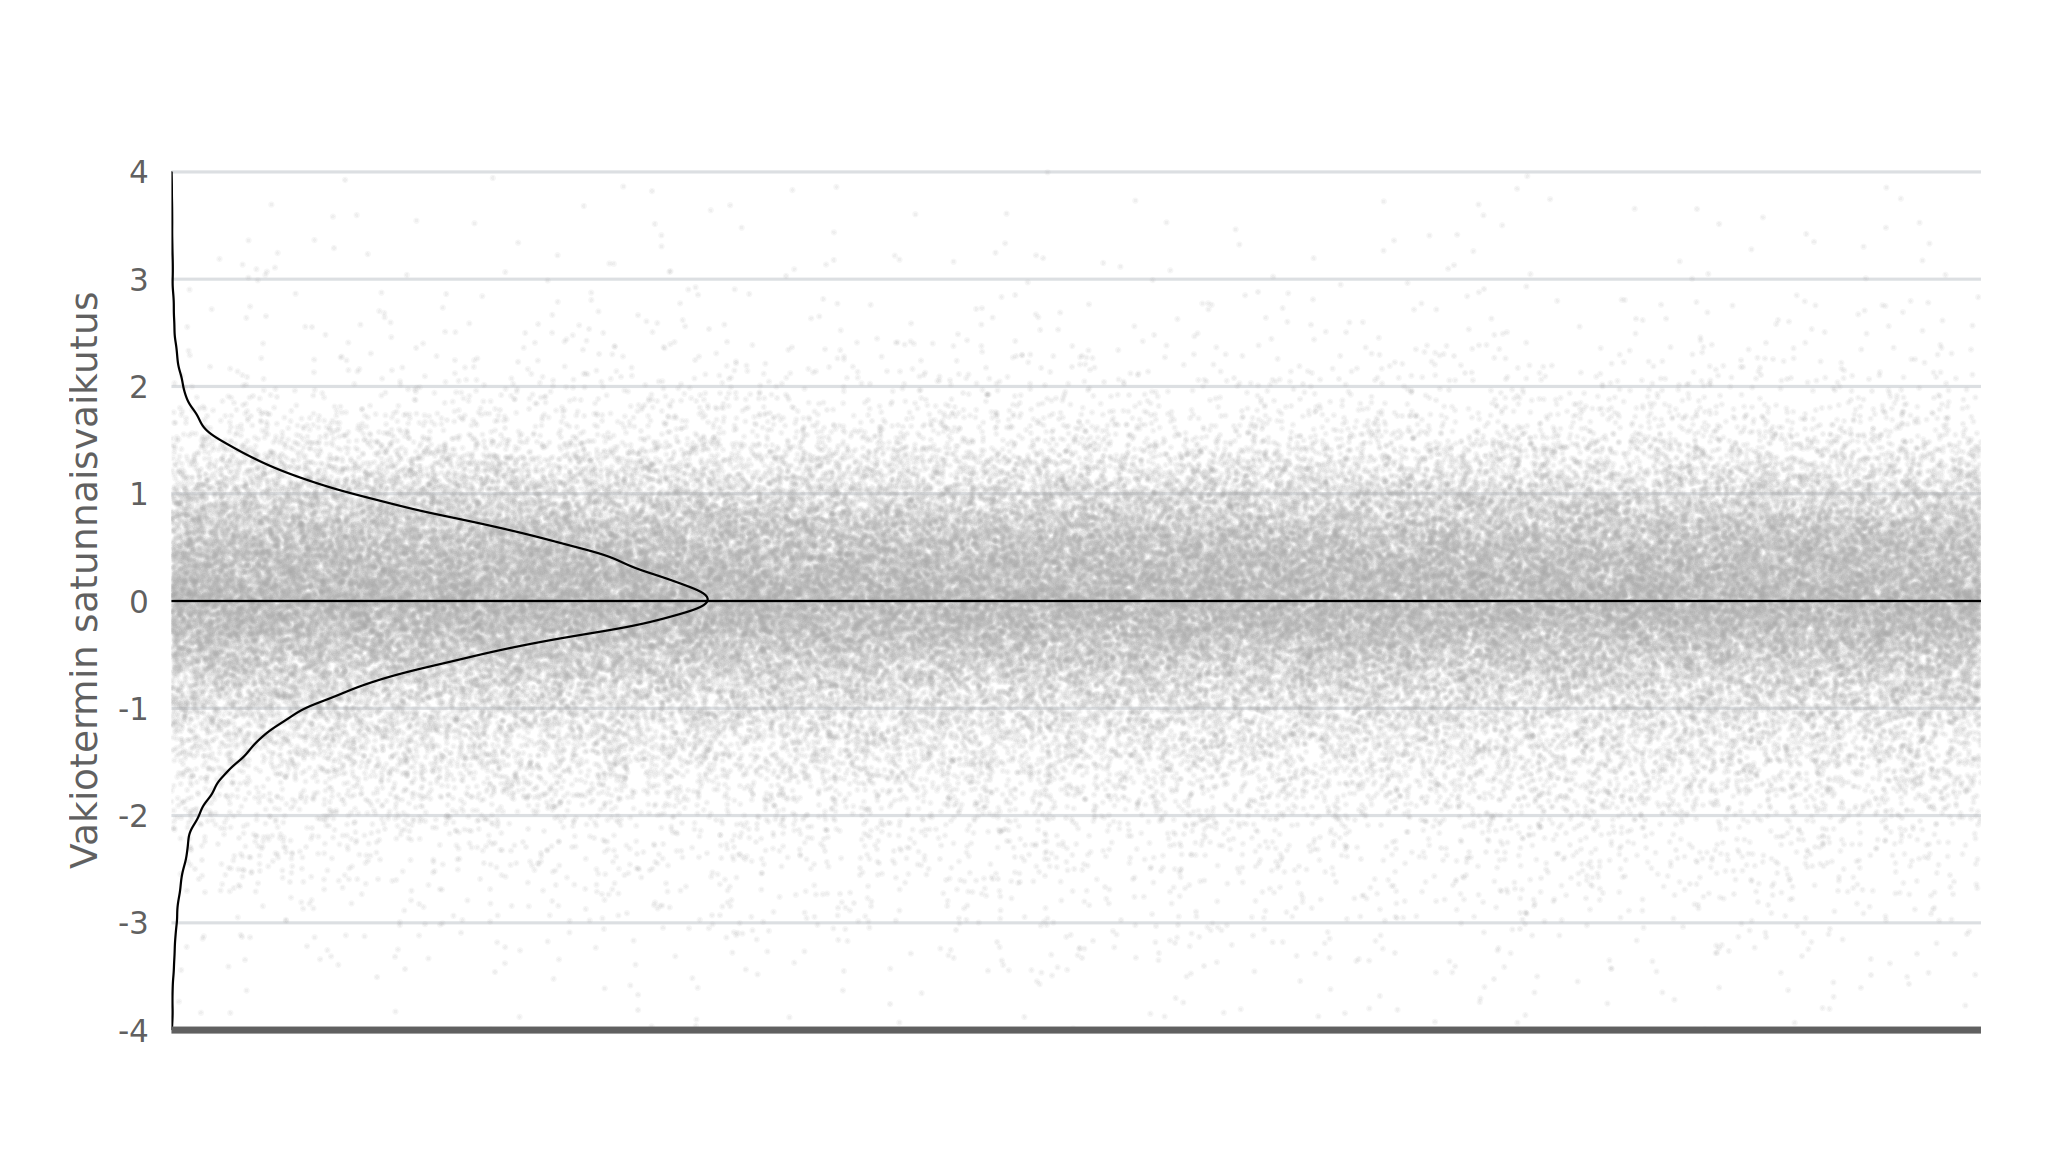
\includegraphics[scale=0.8]{kuvaajat/lme2_vakio_satunnaisvaikutukset.png}
  \caption{Satunnaisvaikutusten mallin vakiotermin ennustetut satunnaisvaikutukset ja tiheysfunktion Gaussin ydinestimaatti}
  \label{fig:lme2_vakio_ranef}
\end{figure}

\begin{figure}[H]
\centering
  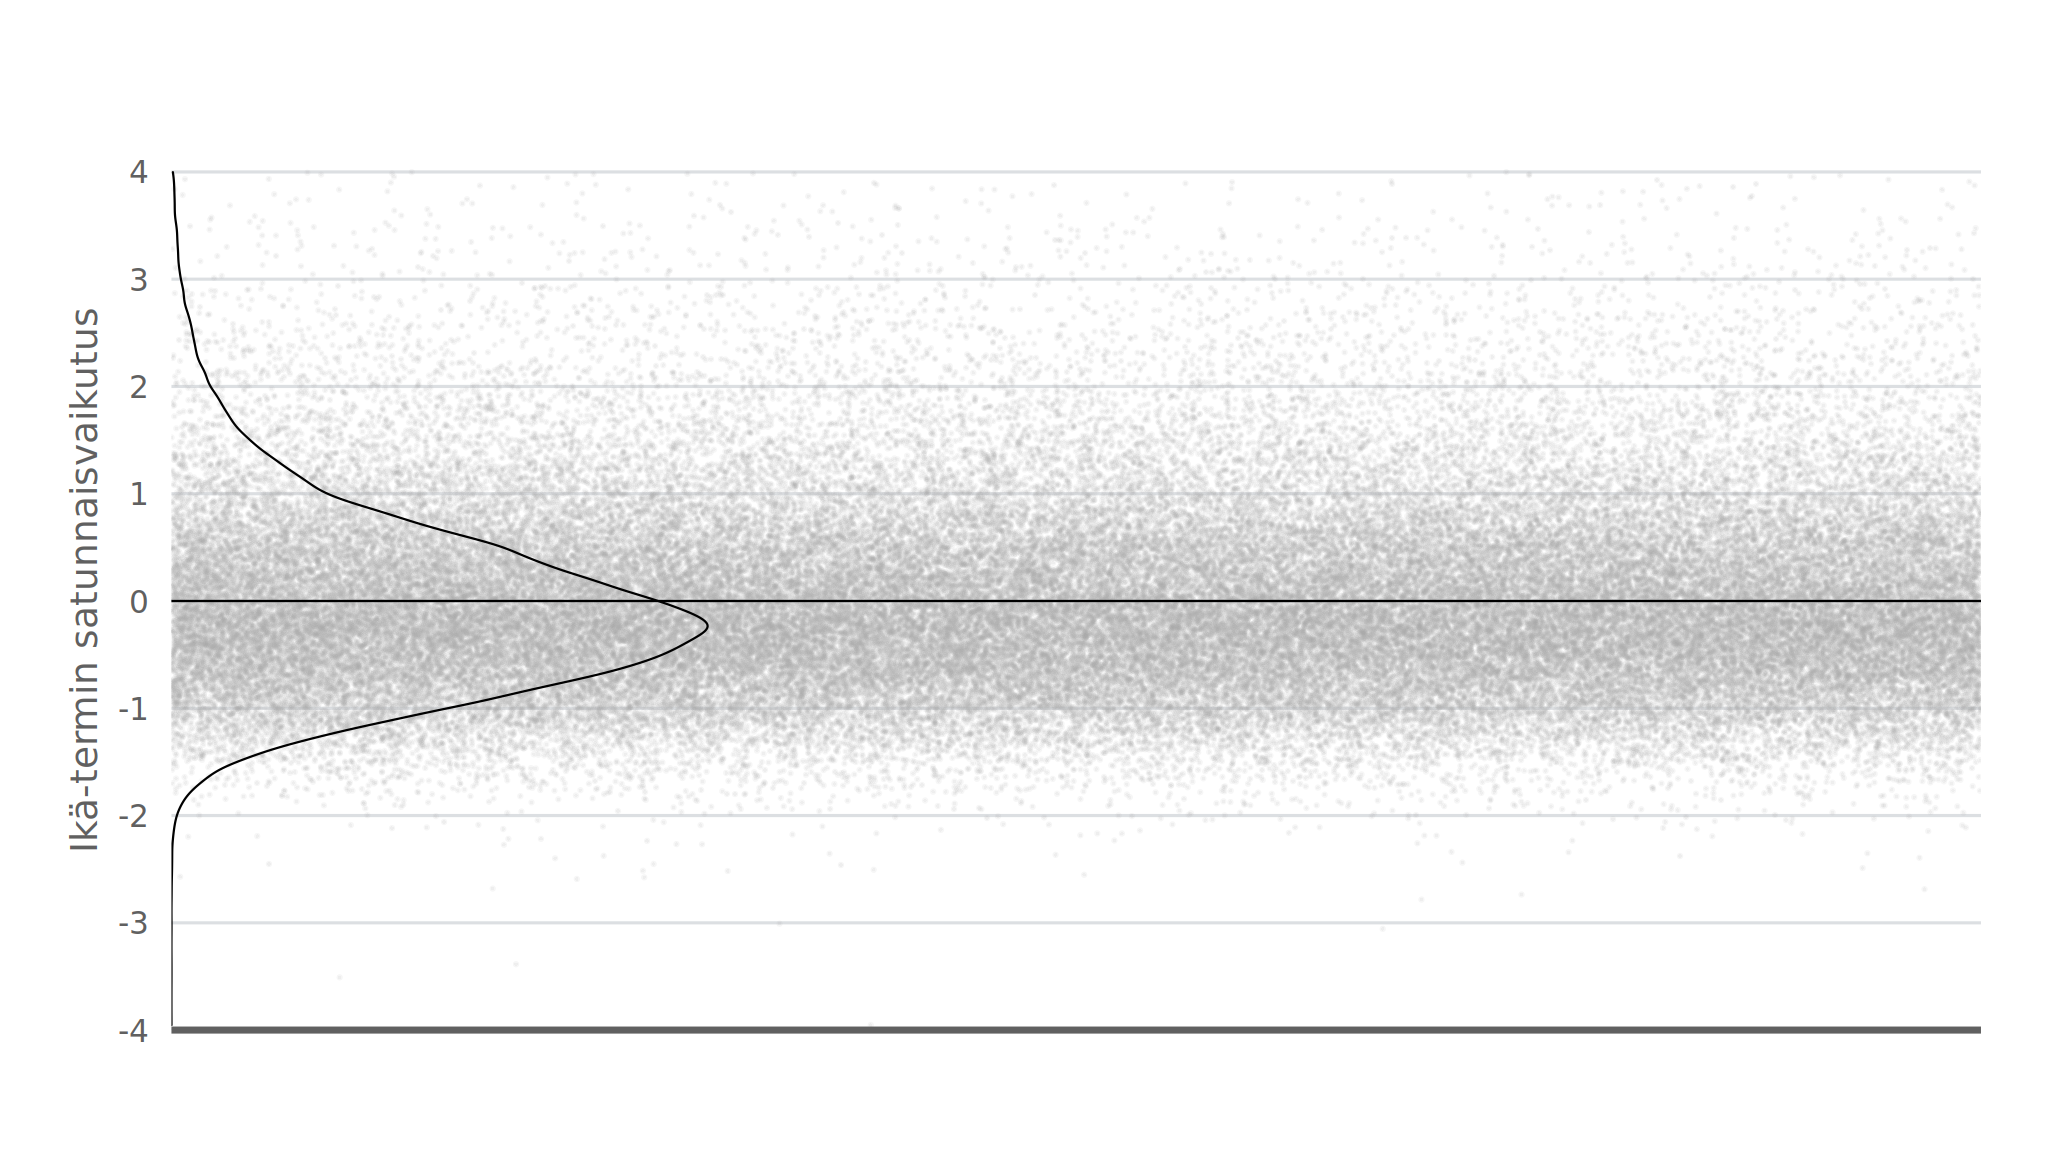
\includegraphics[scale=0.8]{kuvaajat/lme2_ika_satunnaisvaikutukset.png}
  \caption{Satunnaisvaikutusten mallin LSM~\ref{eq:lme2} iän ennustetut satunnaisvaikutukset ja tiheysfunktion Gaussin ydinestimaatti}
  \label{fig:lme2_ika_ranef}
\end{figure}

Pienemmän varianssin lisäksi residuaalien jakauma (Taulukko~\ref{fig:lme2_resid}) näyttää vastaavan jakaumaoletuksia huomattavasti edeltävää mallia paremmin, joskin lopullinen arvio vaatii tarkempaa tarkastelua. Tähän palamme lopullisen mallin arvioinnissa.\\

\begin{figure}[H]
\centering
  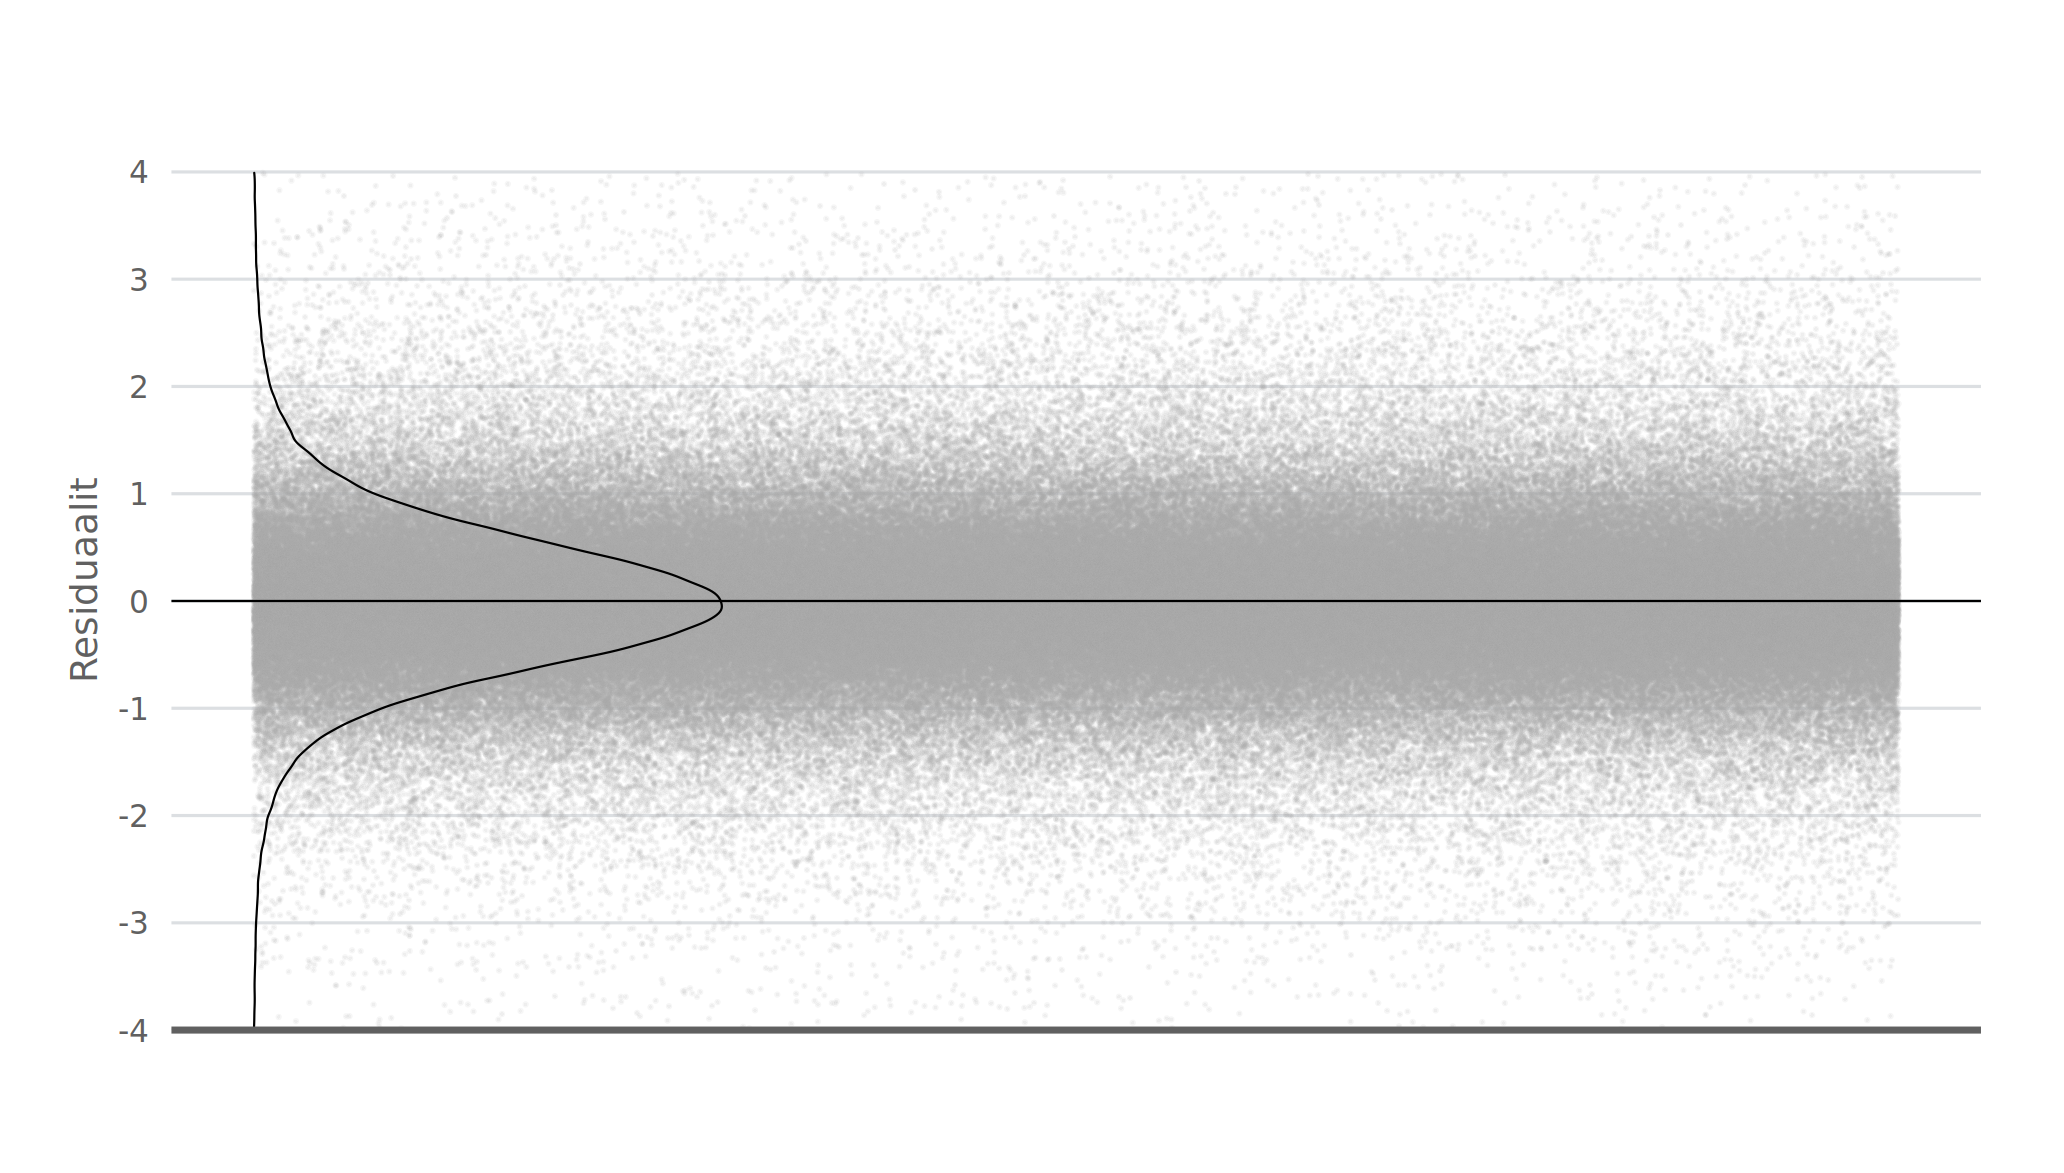
\includegraphics[scale=0.8]{kuvaajat/lme2_residuaalit.png}
  \caption{Satunnaisvaikutusten mallin LSM~\ref{eq:lme2} yksilökohtaisten mittausten Pearson-residuaalit ja tiheysfunktion Gaussin ydinestimaatti}
  \label{fig:lme2_resid}
\end{figure}

Satunnaisvaikutusten malli on osoittanut positiivista parannusta kiinteiden vaikutusten malliin verrattuna, joskin joitakin perustavia kysymuksiä mallin oletusten toteutumisesta ovat vielä jääneet vastaamatta.\\

Taulukon~\ref{table:lme_summary} Bayesin informaatiokriteerin (BIC) perusteella satunnaisvaikutusten malli (LSM~\ref{eq:lme2}), parametrien määrä huomioiden, osoittaa huomattavasti parempaa sopusointua aineistoon suhteen verrattuna kiinteiden vaikutusten malliin (LSM~\ref{eq:lme1}). Vertailuna taulukossa myös alustavan lineaarisen mallin (LM~\ref{eq:lm3}) tuloksia, joihin nähden molemmat lineaaristen sekamallien ryhmään kuuluvat mallit osoittavat merkittävää parannusta. \\

\begin{table}[H]
\centering
\begin{tabular}{lrrrr}
\toprule
Malli & $df$ & $l(\bm{\beta})$ & AIC & BIC\\
\midrule
LM~\ref{eq:lm3} & 5 & -1032898 & 2065806 & 2065861\\
LSM~\ref{eq:lme1} & 7 & -813634 & 1627282 & 1627359\\
LSM~\ref{eq:lme2} & 9 & -729237 & 1458492 & 1458591\\
\bottomrule
\end{tabular}
\caption{Lineaarisen mallin ja lineaaristen sekamallien vapausasteiden, log-uskottavuuksien ja informaatiokriteerien vertailu}
\label{table:lme_summary}
\end{table}

Valitsemme mallin LSM~\ref{eq:lme2} seuraavan vaiheen tarkasteluun, jossa tutkimme tarkemmin residuaalien kovarianssirakennetta.

\subsubsection{Residuaalien kovarianssirakenteen valinta}
\label{ssb:reskovar}

\cite{pinheiro00} tuovat esiin, että \cite{laird82} mukainen lineaarisen sekamallin määrittely tuo huomattavaa joustavuutta satunnaisvaikutusten rakenteen määrittelyyn tilanteissa, joissa yksilökohtaiset residuaalit ovat korreloimattomia ja niiden varianssi on vakio, mutta voi sellaisenaan johtaa ristiriitaisiin tuloksiin tapauksissa, joissa yksilön residuaalit ovat korreloituneita, niiden varianssissa esiintyy heteroskedastisuutta tai molempia samanaikaisesti.\\

Osiossa~\ref{sub:kovarianssirakenteet} totesimme, että matriisiin $\bm{R}_i$ voidaan korreloimattoman diagonaalirakenteen sijaan sisällyttää myös muita rakenteita. \cite{pinheiro00} mukaan tämä käytännössä vaatii kuitenkin lineaarisen sekamallin laajentamista.\\

\cite{pinheiro00} näyttävät, että residuaalien kovarianssimatriisille $\bm{R}_i$ löytyy hajotelma

$$
\bm{R}_i = \bm{W}_i \bm{C}_i \bm{W}_i,
$$

jossa $\bm{W}_i$ on diagonaalimatriisi, joka diagonaalialkiot ovat positiivisia ja $\bm{C}_i$ positiividefiniitti korrelaatiomatriisi, jonka kaikki diagonaalialkiot ovat ykkösiä. \cite{pinheiro00} mukaan hajotelma on residuaalien kovarianssimatriisin tarkastelun kannalta hyödyllinen, sillä sen avulla voimme määritellä yksilön $i$ residuaalelle sekä varianssirakenteen 

$$
\text{Var}(\epsilon_{ij}) = \sigma^2(\bm{W}_i)^2_{jj}
$$

ja korrelaatiorakenteen

$$
\text{cor}(\epsilon_{ij}, \epsilon_{ik}) = (\bm{C}_i)_{jk}.
$$

\cite{pinheiro00} mukaan laajennettuun lineaariseen malliin liittyy kaksi keskeistä huomiota. Ensinnäkin laajennetun mallin estimointi eroaa mm. tämän tutkielman määrittelystä. Toiseksi, laajennetun lineaarisen sekamallin vasteen kovarianssimatriisissa

$$
\text{Cov}(\bm{y}_i) = \bm{Z}_i \bm{G} \bm{Z}_i^\top +  \bm{W}_i \bm{C}_i \bm{W}_i,
$$

satunnaisvaikutusten komponentti $\bm{Z}_i \bm{G} \bm{Z}_i^\top$ ja yksilökohtaisten residuaalien komponentti $\bm{W}_i \bm{C}_i \bm{W}_i$ kilpailevat osin keskenään, tulee komponenttien määrittely suunnitella huolella ja kiinnittää huomiota mm. monimutkaisten satunnaisvaikutusten ja varianssi- ja korrelaatiorakenteiden samanaikaiseen mallintamiseen.\\

Näitä huomioita noudattaen, varianssin heteroskedastisuuden ja residuaalien korreloituneisuuden tarkastelu on tärkeä vaihe, mutta suhtaudumme suuntaa-antavasti mahdollisiin ehdotuksiin niiden ratkaisemiseksi ja rajaamme \cite{pinheiro00} tarjoaman laajennetun lineaarisen sekamallin määrittelmän tämän tarkastelun ulkopuolelle.\\

Vaikka satunnaisvaikutusmallin residuaalien jakauma vaikutti lupaavalta, mikäli tarkastelemme residuaaleja iän suhteen (Kuva~\ref{fig:lme2_ika_resid}) paljastaa, ettei oletus varianssin homoskedastisuudesta ole pitävä. Silmämääräisesti varianssi vaikuttaa olevan pienempi nuorempana ja kasvavan iän myötä, tosin aivan pienten lasten kohdalla on havaittavissa myös merkittävää harhaa.\\

\begin{figure}[H]
\centering
  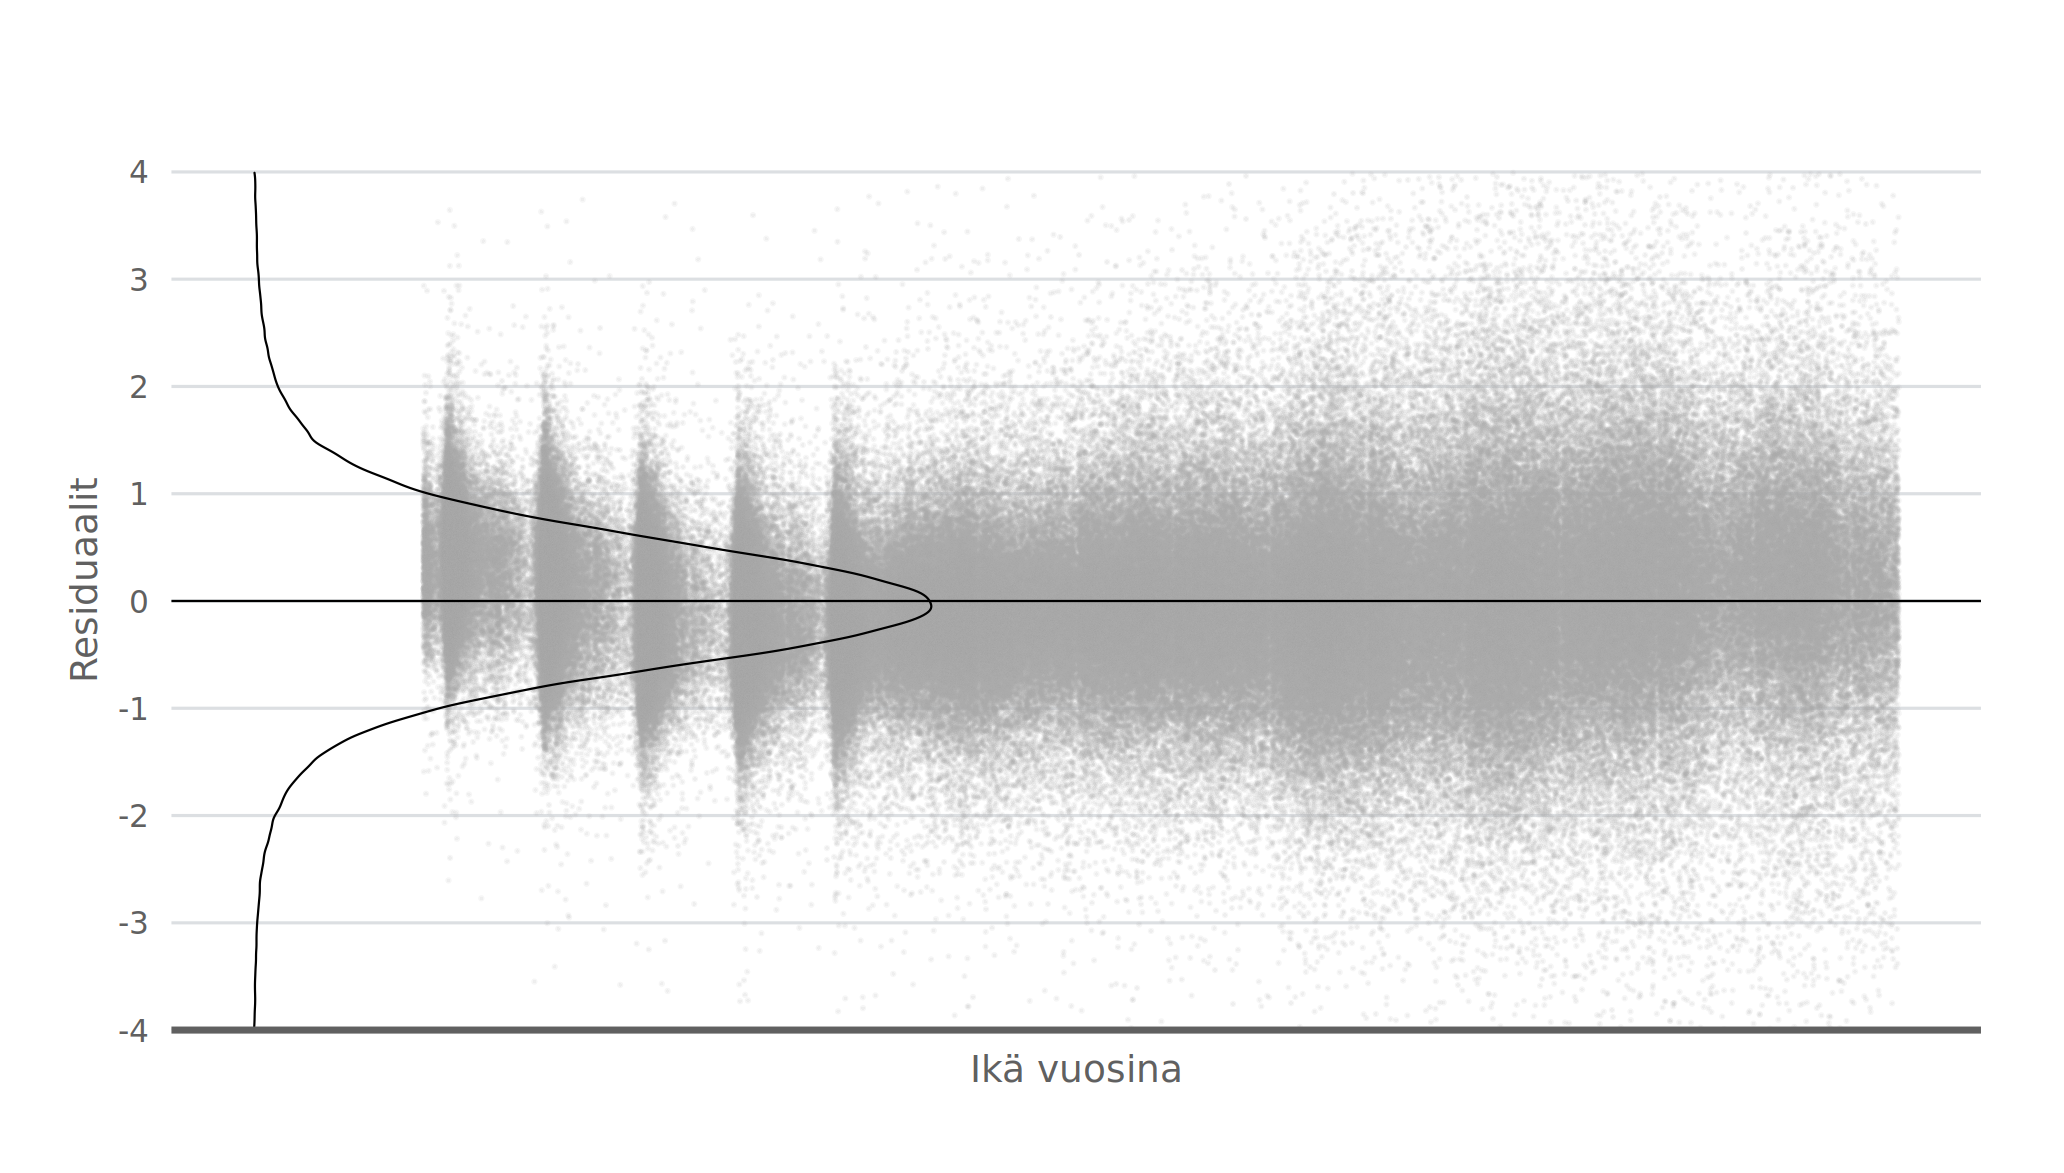
\includegraphics[scale=0.8]{kuvaajat/lme2_ika_residuaalit.png}
  \caption{Satunnaisvaikutusten mallin yksilökohtaisten mittausten Pearson-residuaalit iän suhteen ja tiheysfunktion Gaussin ydinestimaatti}
  \label{fig:lme2_ika_resid}
\end{figure}

Yksilön mittausten välistä autokorrelaatiota voimme \cite{pinheiro00} mukaan tarkastella autokorrelaatiofunktion avulla. Oletamme, että virhetermit $\epsilon_{ij}, \epsilon_{ik}$ ovat riippuvat sijainneista $p_{ij}, p_{ik}$, jonkin etäisyyden $d(p_{ij}, p_{ik})$ mukaan. Voimme siten määritellä autokorrelaatiofunktion $h$

$$
\text{cor}(\epsilon_{ij}, \epsilon_{ik}) = h(d(p_{ij}, p_{ik}), \bm{\rho})),
$$

jossa $d$ on jokin etäisyysfunktio ja $\bm{\rho}$ korrelaatioparametrien vektori.\\

Tarkastellaksemme autokorrelaatiota esimerkiksi iän perusteella, voimme määritellä sijainneiksi $p_{ij}, p_{ik}$ yksilön $i$ iän mittauksilla $j$ ja $k$, sekä etäisyydeksi $d$ euklidisen etäisyyden, eli yksiulotteisessa tapauksessa erotuksen itseisarvon $|\text{IKÄ}_{ij} - \text{IKÄ}_{ik}|$ mittausten $j$ ja $k$ välillä.\\ 

\cite{pinheiro00} osoittavat, että mittausten samankaltaisuutta perustuen määriteltyyn etäisyyteen $s$ korrelaatioparametreillä $\bm{\rho}$ voidaan tarkastella semivariogrammilla (Kuva ~\ref{fig:lme2_vario})

$$
\gamma(s, \rho) = 1 - h(s, \bm{\rho})\\
$$

\begin{figure}[H]
\centering
  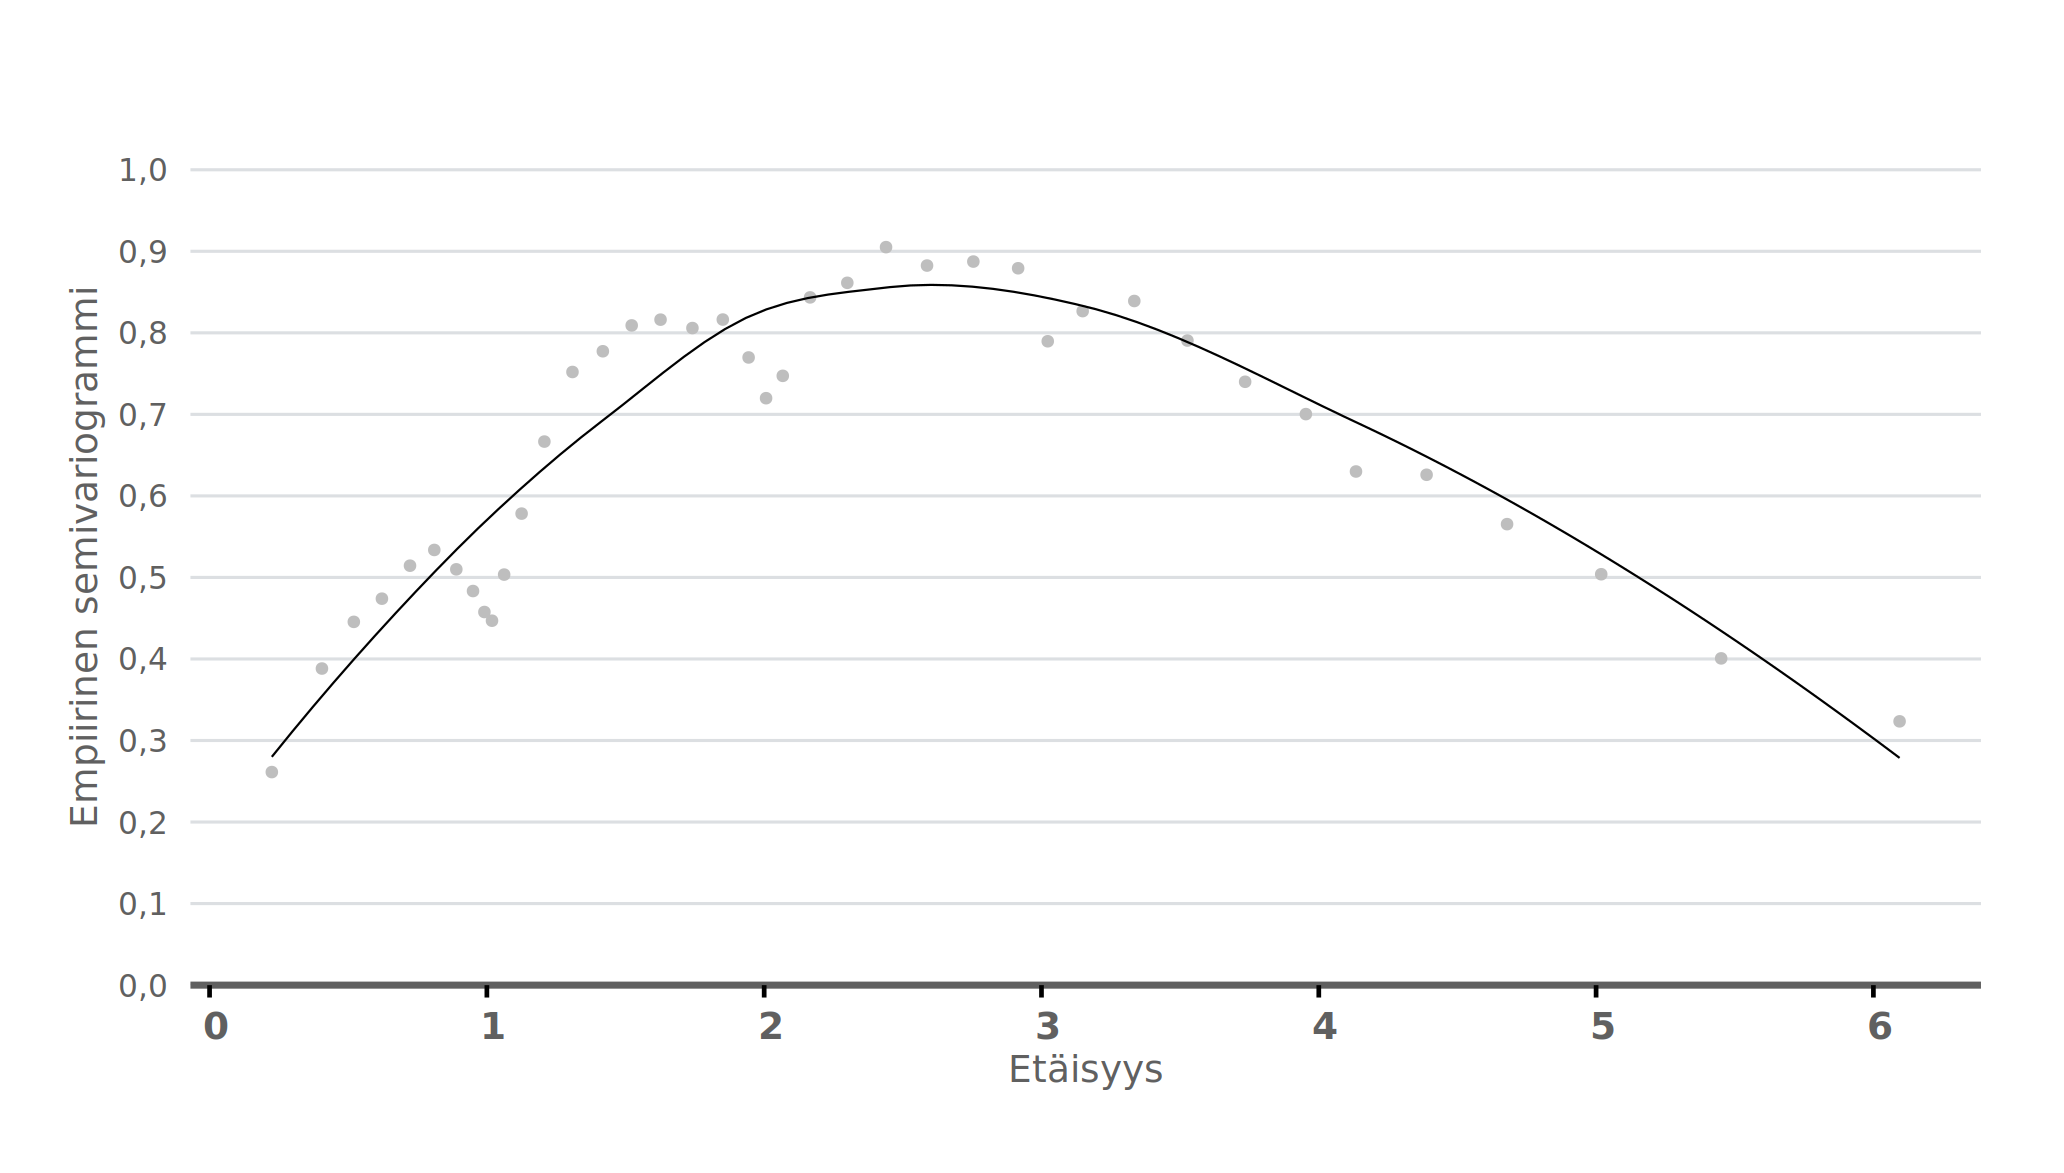
\includegraphics[scale=0.8]{kuvaajat/lme2_vario.png}
  \caption{Satunnaisvaikutusten mallin empiirinen semivariogrammi ($\hat{\gamma}$)}
  \label{fig:lme2_vario}
\end{figure}

Semivariogrammin pisteet kuvaavat kukin noin 20 000 Pearsonin residuaaliparin perustuvaa samankaltaisten havaitoparien klusteria ja käyrä kuvaa LOESS-tasoitettua trendiä suhteessa residuaaliparin sijaintien etäisyyteen. Matalammat semivariogrammin arvot viittaavat samankaltaisuuteen ja korkeammat arvot erilaisuuteen.\\

Tarkastelun perusteella aineistossa ilmenee kohtalaisen voimakasta autokorrelaatiota yksilön mittausten välillä suhteessa mittausten väliseen ajalliseen etäisyyteen. Noin kolmeen vuoteen saakka tarkastelu tukee intuitiota, että lähellä olevat arvot ovat samankaltaisempia.\\

Kolmen vuoden jälkeen samankaltaisuus vaikuttaisi vastoin odotuksia lisääntyvän, mikä \cite{pinheiro00} mukaan voi usein johtua estimaattien epäluotettavuudesta pitkillä etäisyyksillä, mutta se voi kertoa myös ongelmista mallin oletusten suhteen.\\

On selviä viitteitä, että varianssin heteroskedastisuuteen ja residuaalien autokorrelaatioon olisi syytä kiinnittää huomiota. Tarkastelemme molempia ongelmia esimerkkien kautta ja vertaamme lopullisen mallin suhteen mahdollisia ratkaisuja, mutta syvällinen analyysi on rajattu tutkielman ulkopuolelle.\\

Kuten aiempi tarkastelu antoi viiteitä (Kuva~\ref{fig:lme2_ika_resid}), varianssia voi olla perusteltua tarkastella iän funktiona. Mikäli oletamme varianssin iän lineaariseksi funktioksi, voimme \cite{pinheiro00} mukaillen määritellä varianssiksi

$$
\text{Var}(\epsilon_{ij}) = \sigma^2\text{IKÄ}_{ij}
$$

ja siten varianssifunktioksi

$$
g(\text{IKÄ}_{ij}) = \sqrt{\text{IKÄ}_{ij}}.
$$

Tällöin saamme varianssipainoiksi $1/\sqrt{\text{IKÄ}_{ij}}$, joiden avulla voimme sovittaa uudelleen satunnaisvaikusten mallin pyrkien painottamaan varianssia heteroskedastisuuden vähentämiseksi. Kuvassa~\ref{fig:lme2_varfunc} varianssipainokertoimien muutos kuvattu iän suhteen. \\

\begin{figure}[H]
\centering
  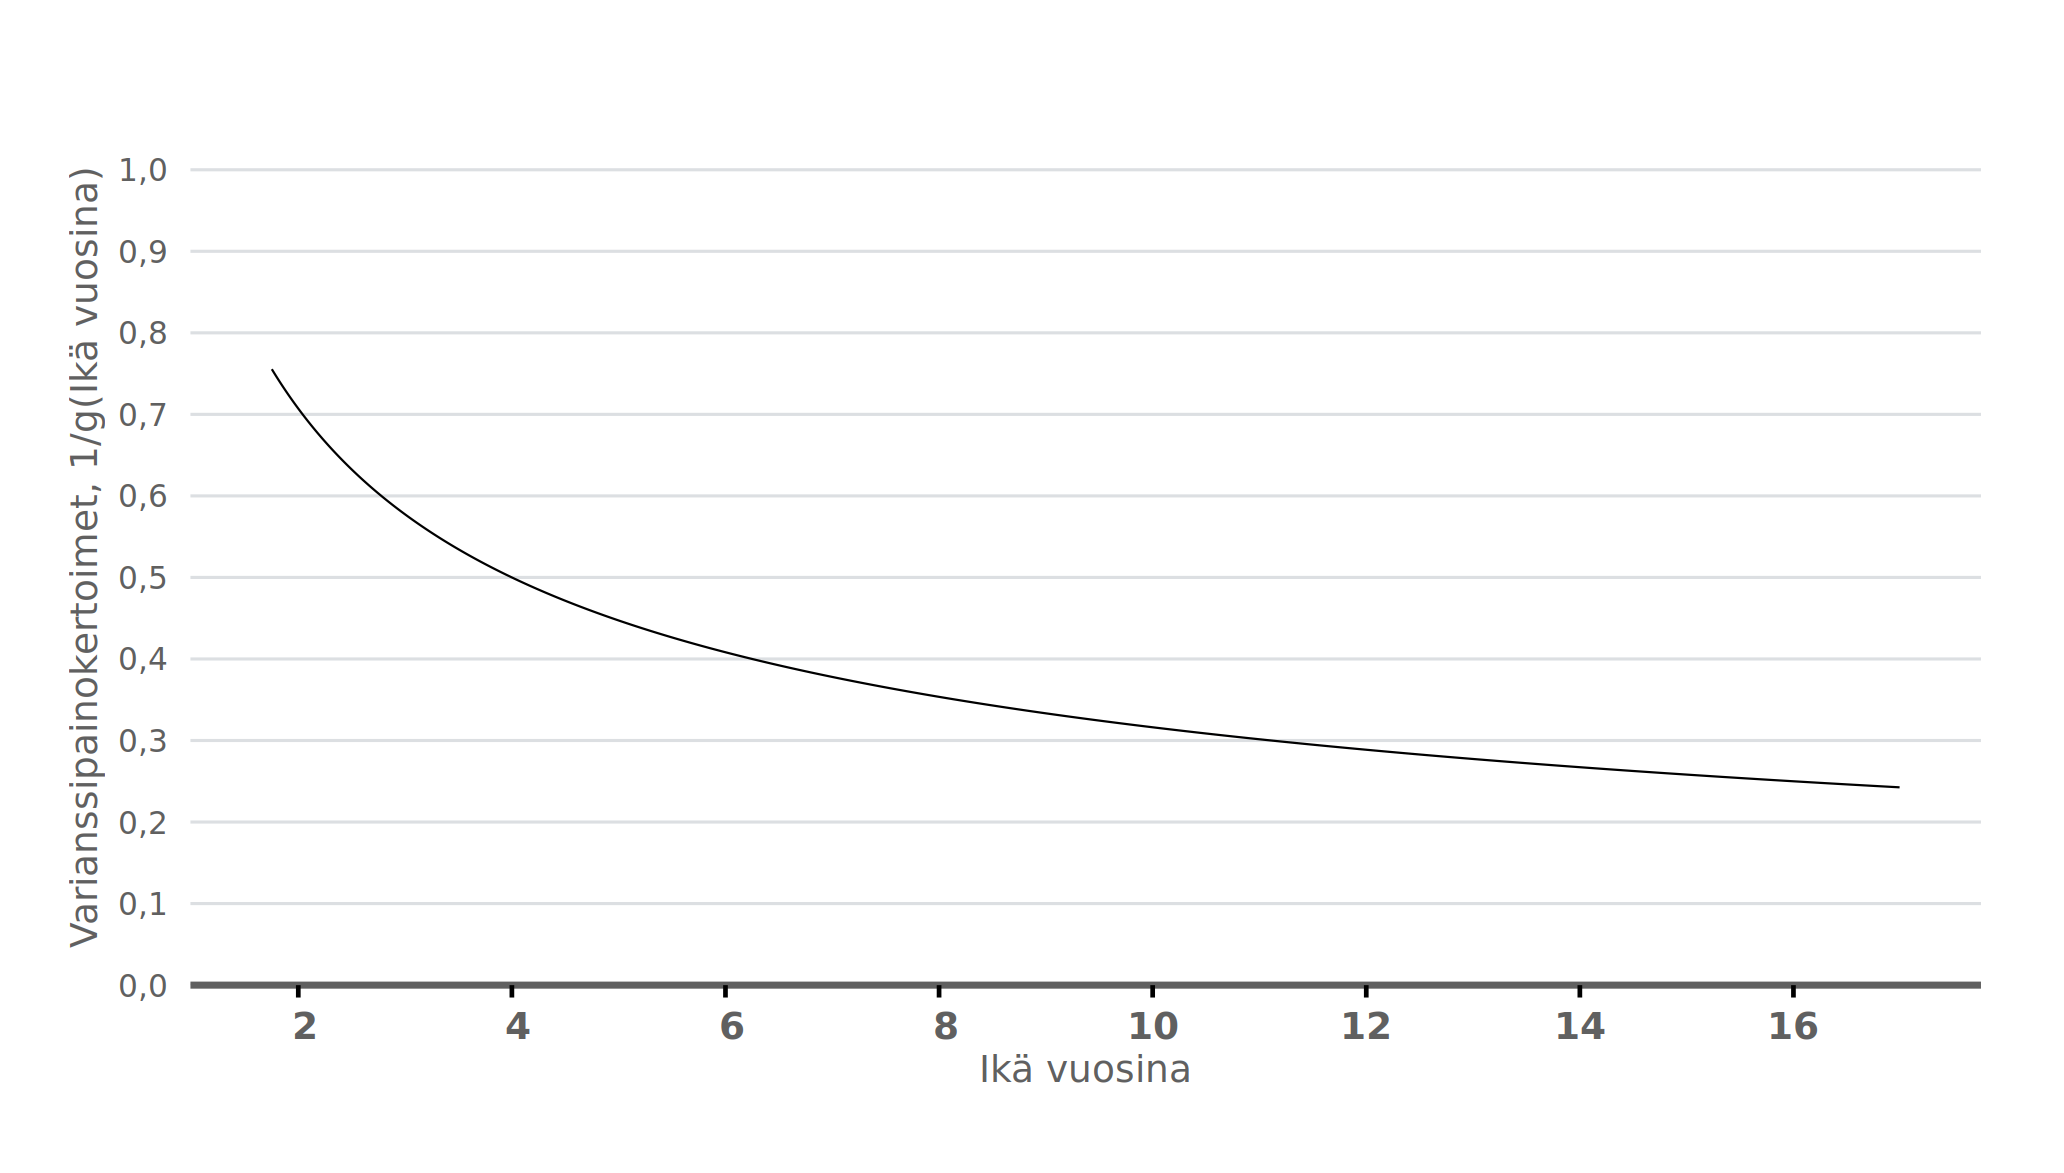
\includegraphics[scale=0.8]{kuvaajat/lme2_varfunc.png}
  \caption{Varianssipainokertoimien $1/g(\text{IKÄ}_{ij})$ muutos iän suhteen}
  \label{fig:lme2_varfunc}
\end{figure}

Satunnaisvaikutusten varianssipainotetun mallin residuaalien vaihtelu (Kuva ~\ref{fig:lme2_ika_v_resid}) on hieman parantunut suuremmilla iän arvoilla, erityisesti kuvaajan alkupäässä residuaalivaihtelu on vääristynyttä. Heteroskedastisuuden tasoittuminen on havaittavissa myös semivariogrammin estimaateissa (Kuva ~\ref{fig:lme2_v_vario}), mutta autokorrelaatio vaikuttaa pysyneen muuttumattomana.\\

\begin{figure}[H]
\centering
  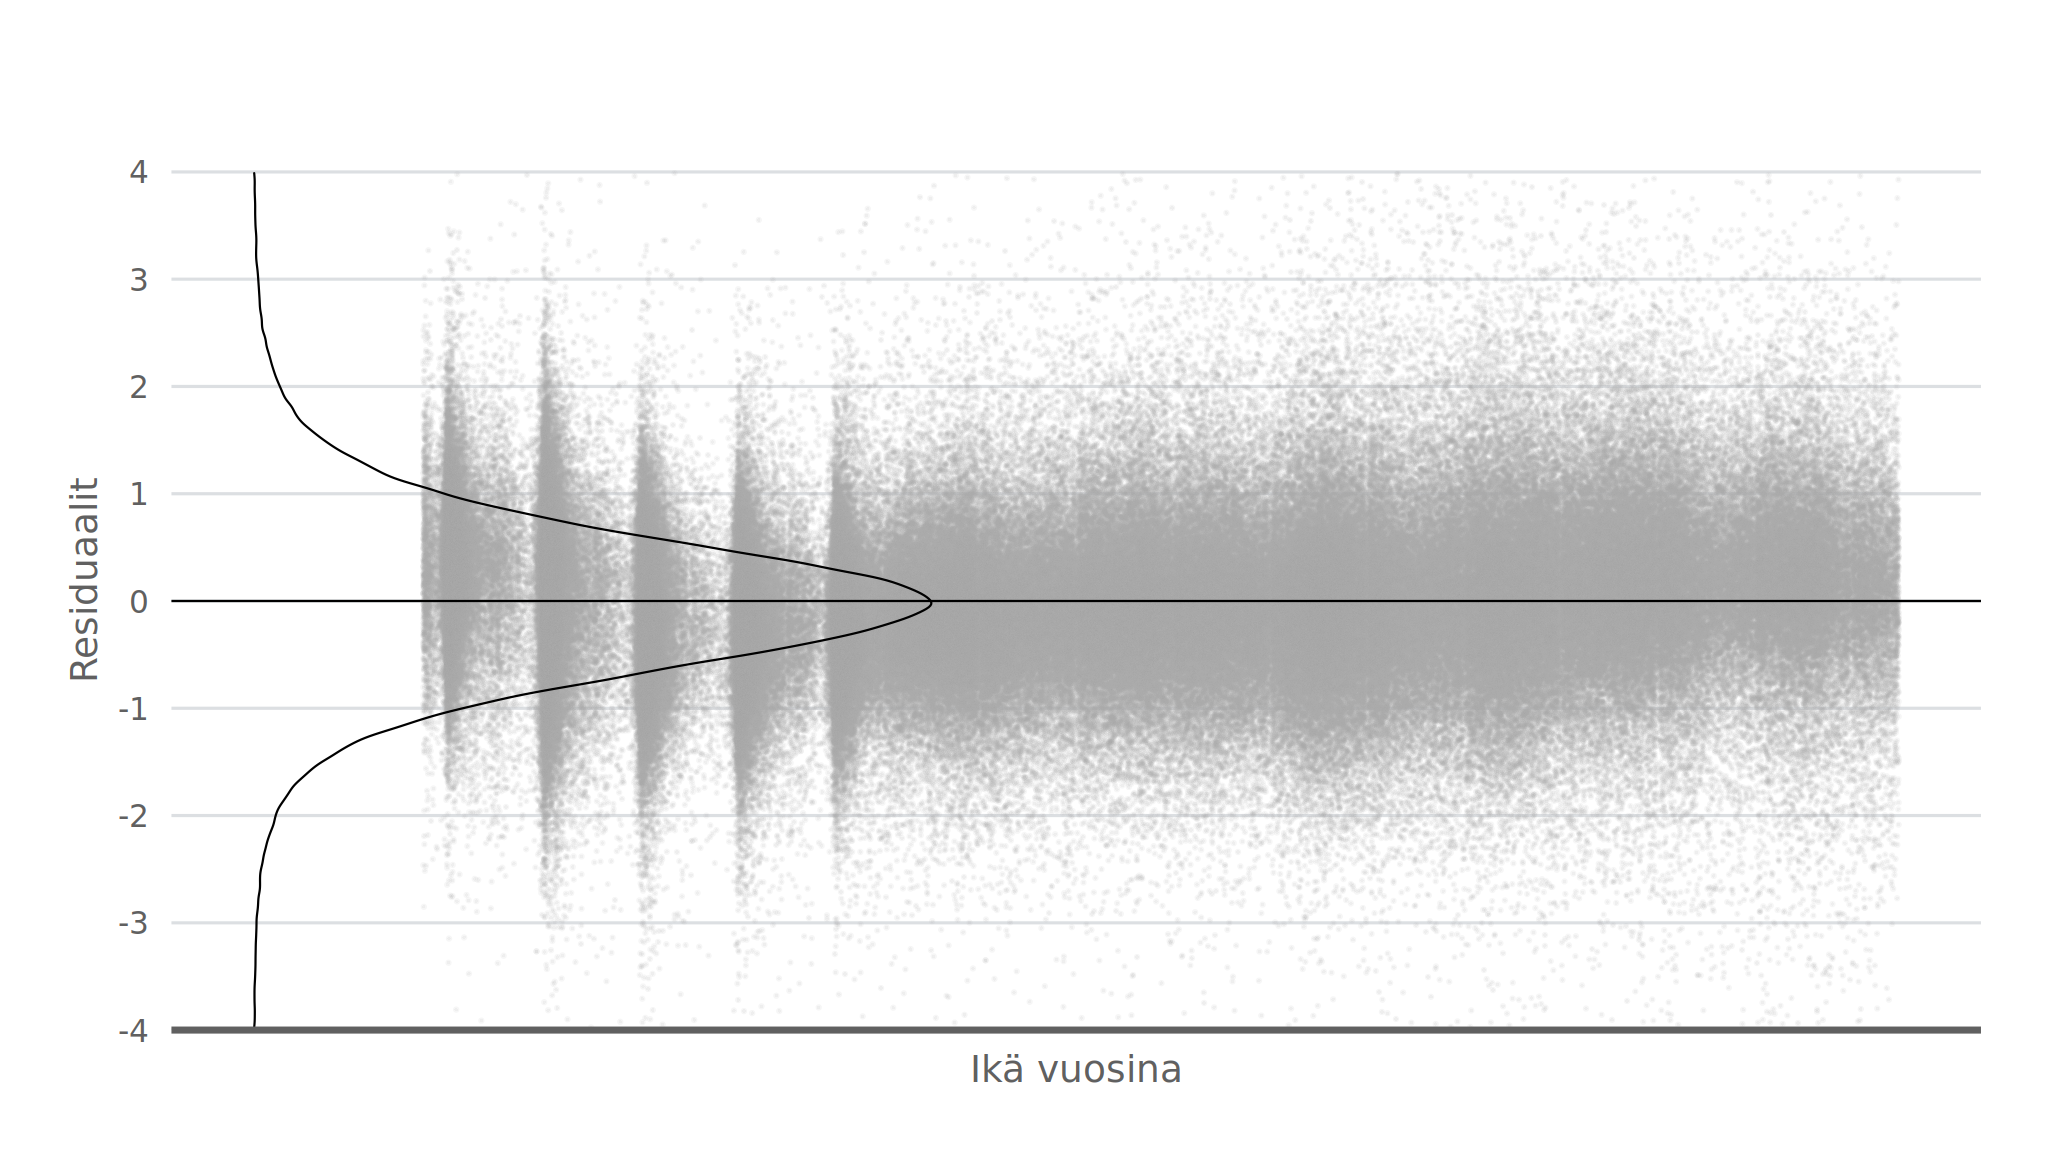
\includegraphics[scale=0.8]{kuvaajat/lme2_ika_v_residuaalit.png}
  \caption{Satunnaisvaikutusten varianssipainotetun mallin yksilökohtaisten mittausten Pearson-residuaalit iän suhteen ja tiheysfunktion Gaussin ydinestimaatti}
  \label{fig:lme2_ika_v_resid}
\end{figure}

\begin{figure}[H]
\centering
  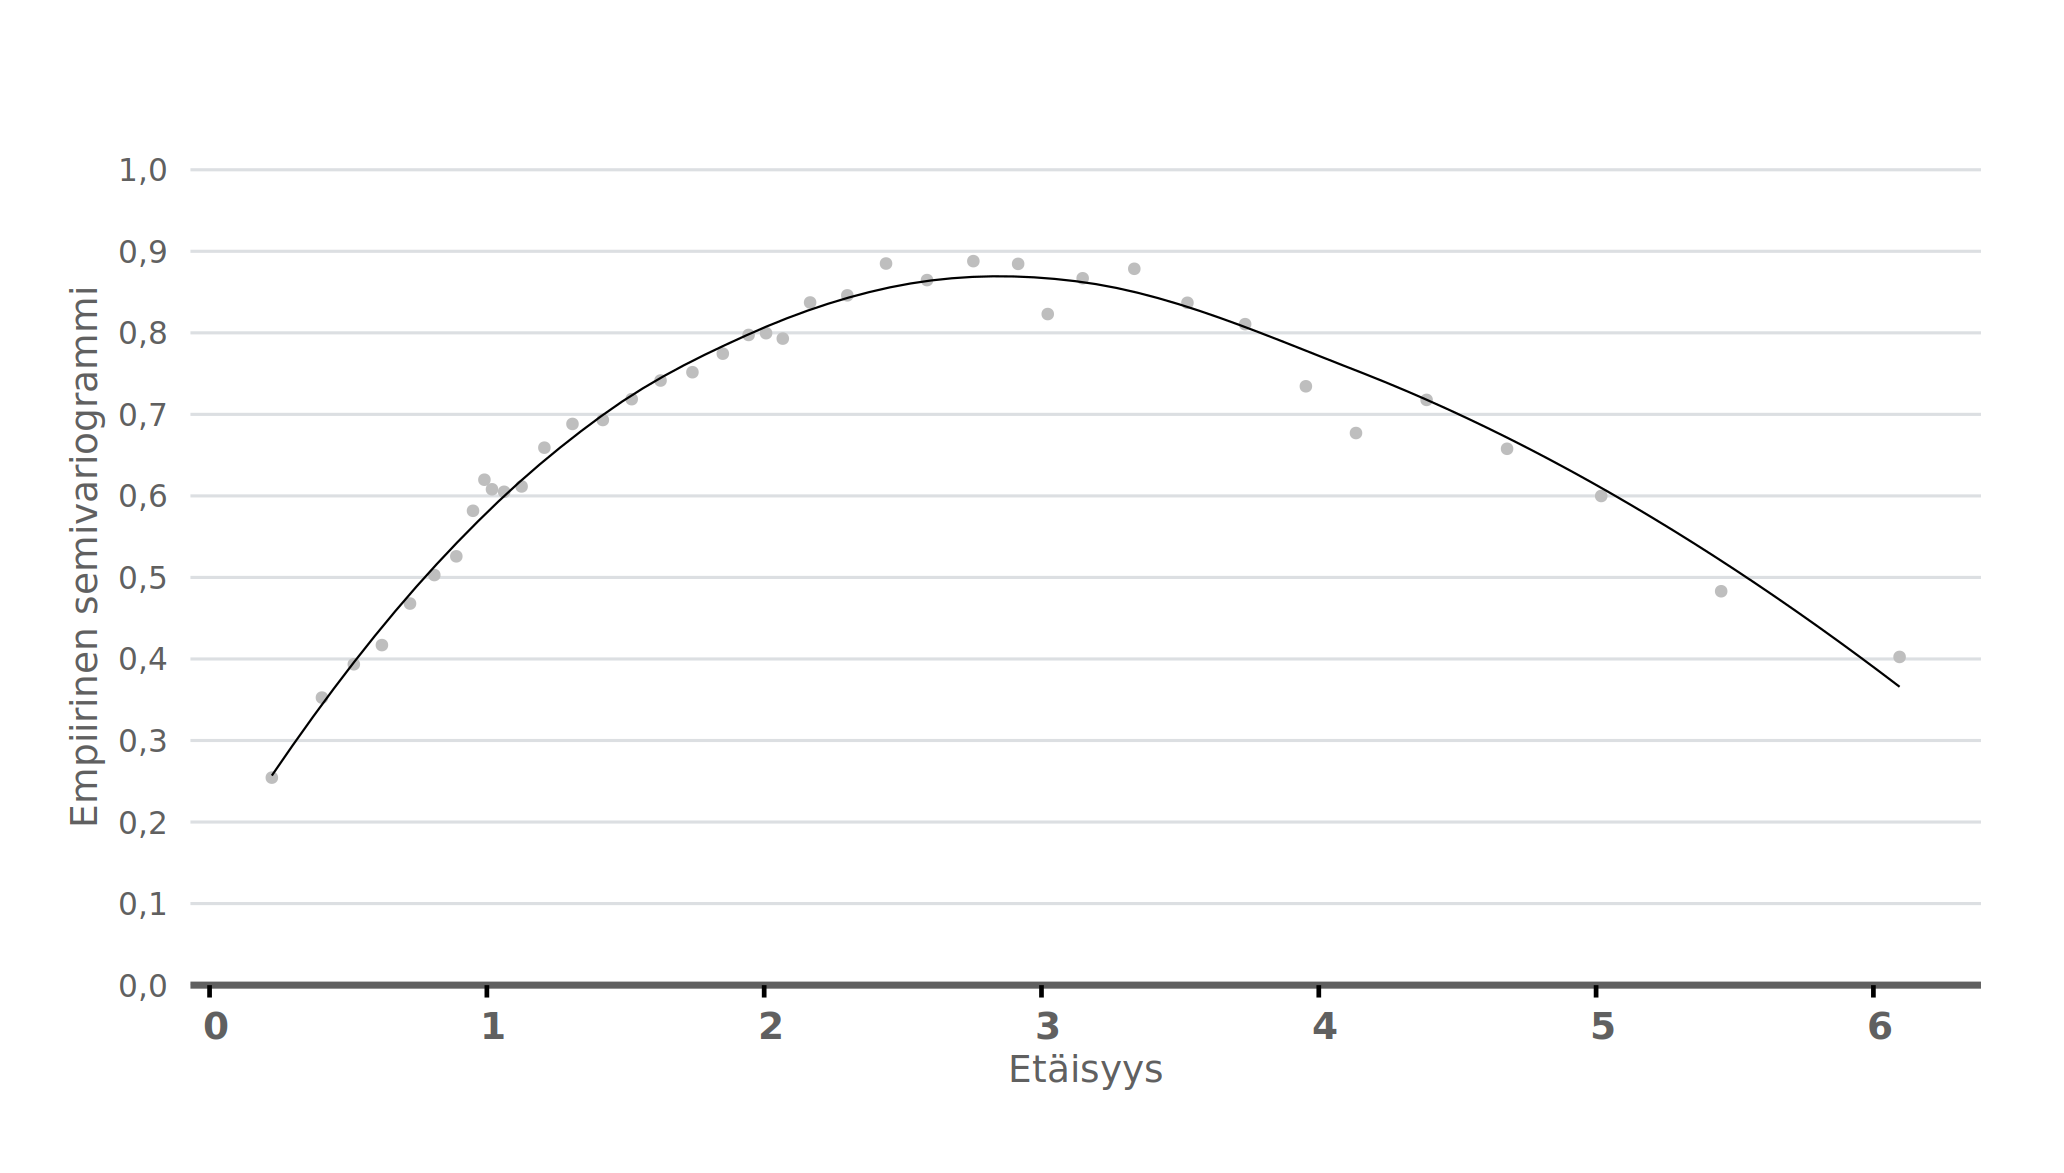
\includegraphics[scale=0.8]{kuvaajat/lme2_v_vario.png}
  \caption{Satunnaisvaikutusten varianssipainotetun mallin empiirinen semivariogrammi ($\hat{\gamma}$)}
  \label{fig:lme2_v_vario}
\end{figure}

Kovarianssirakenteita käsittelevässä osiossa (~\ref{sub:kovarianssirakenteet}) esittelimme ensimmäisen asteen autoregressiivisen mallin AR(1) kovarianssirakenteen olevan riittämätön epätasapainoiseen aineistoon. \cite{pinheiro00} määrittelevät ensimmäisen asteen autoregressiiviseksi autokorrelaatiofunktioksi $h(k,\phi)=\phi^k$, jossa korrelaatioparametri $\phi$ on \textit{lag-1}-korrelaatiokerroin ja $k=0,1,\dots n_i$ Tämä voidaan heidän mukaansa yleistää jatkuvan autoregressiivisen mallin CAR(1) autokorrelaatiofunktioksi $h(s,\phi)=\phi^s$, jossa $s>0$ ja $\phi>0$.

Korrelaatioparametrin estimaatiksi saamme $\hat{\phi} = 0,591$, mikä viittaa kohtalaisen korkeaan autokorrelaatioon. Kuvan~\ref{fig:lme2_corfunc} mukaan korrelaatio laskee jyrkemmin noin kahden vuoden etäisyyteen saakka, jonka jälkeen se suppenee kohti nollaa. Tämä on ensimmäisten kolmen vuoden osalta likimain yhtäpitävää empiirisen semivariogrammin tulosten suhteen, mutta ei vastaa tilannetta yli kolmen vuoden etäisyyksillä.\\

\begin{figure}[H]
\centering
  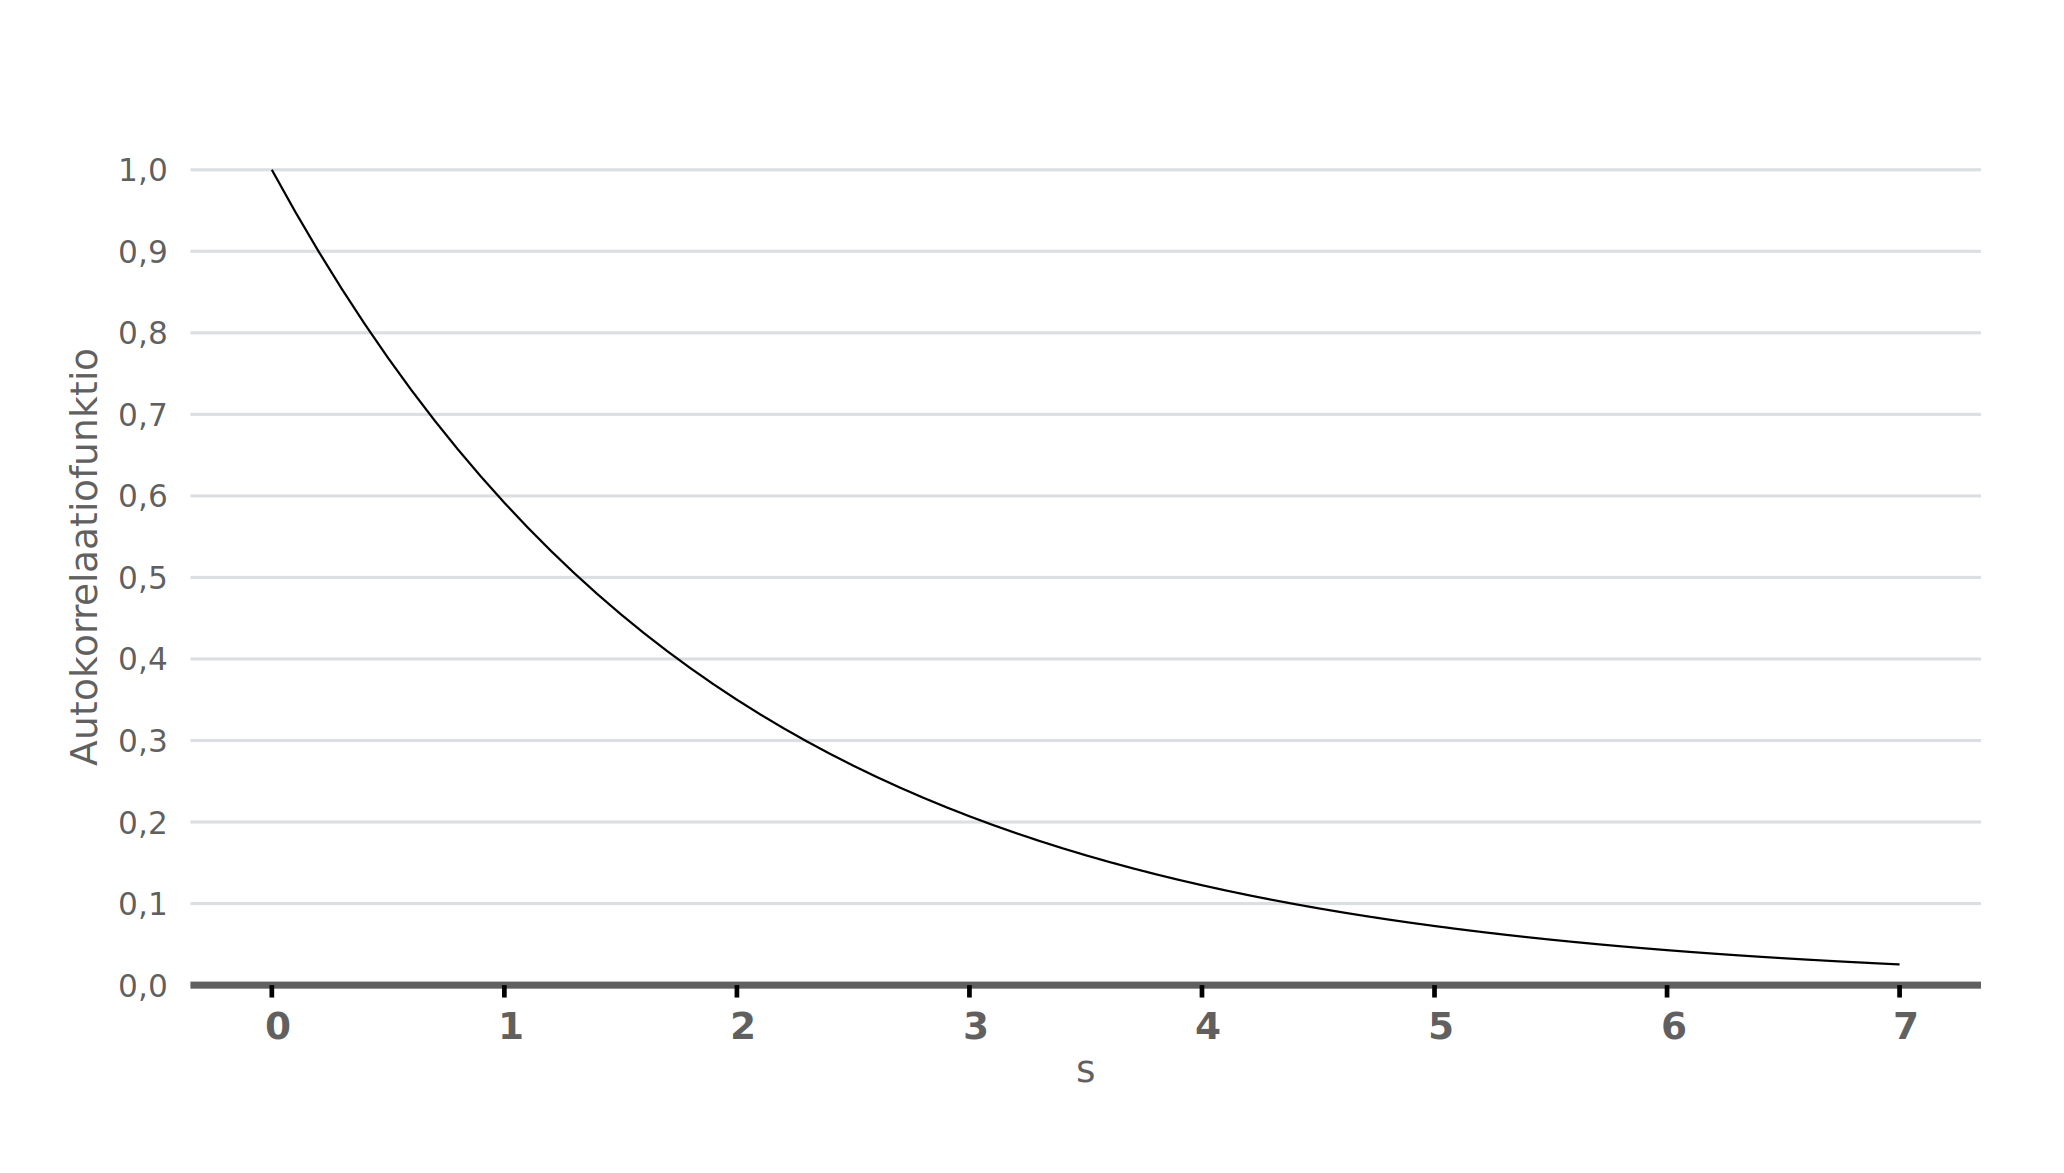
\includegraphics[scale=0.8]{kuvaajat/lme2_corfunc.png}
  \caption{CAR(1)-mallin autokorrelaatiofunktion $\hat{\phi}^s$ muutos $s$ suhteen, jossa $s>0$ on mittausten etäisyys vuosina ja $\hat{\phi} = 0,591$}
  \label{fig:lme2_corfunc}
\end{figure}

Tarkastellaan satunnaisvaikutusten varianssipainotettua mallia, kun mallissa huomioidaan residuaalien autokorrelaatio, olettaen residuaaliparien etäisyydelle CAR(1)-mallin mukainen autokorrelaatiofunktio estimoidulla korrelaatioparametrilla $\hat{\phi} = 0,591$. Kutsumme varianssipainotettua residuaalien autokorrelaation huomioivaa mallia jatkossa laajennetuksi malliksi.\\

Residuaaleissa on havaittavissa merkittävää parannusta, vaikka varianssissa ilmeneekin iän suhteen aaltoilua (Kuva~\ref{fig:lme2_ika_vc_resid}). Semivariogrammin perusteella autokorrelaatiota ole saatu täysin eliminoitua, mutta sen arvot ovat tasoittuneet huomattavasti (Kuva~\ref{fig:lme2_vc_vario}). Myös kaukana toisistaan sijaitsevien mittausten epäilyttävä korreloituneisuus on lieventynyt.\\

\begin{figure}[H]
\centering
  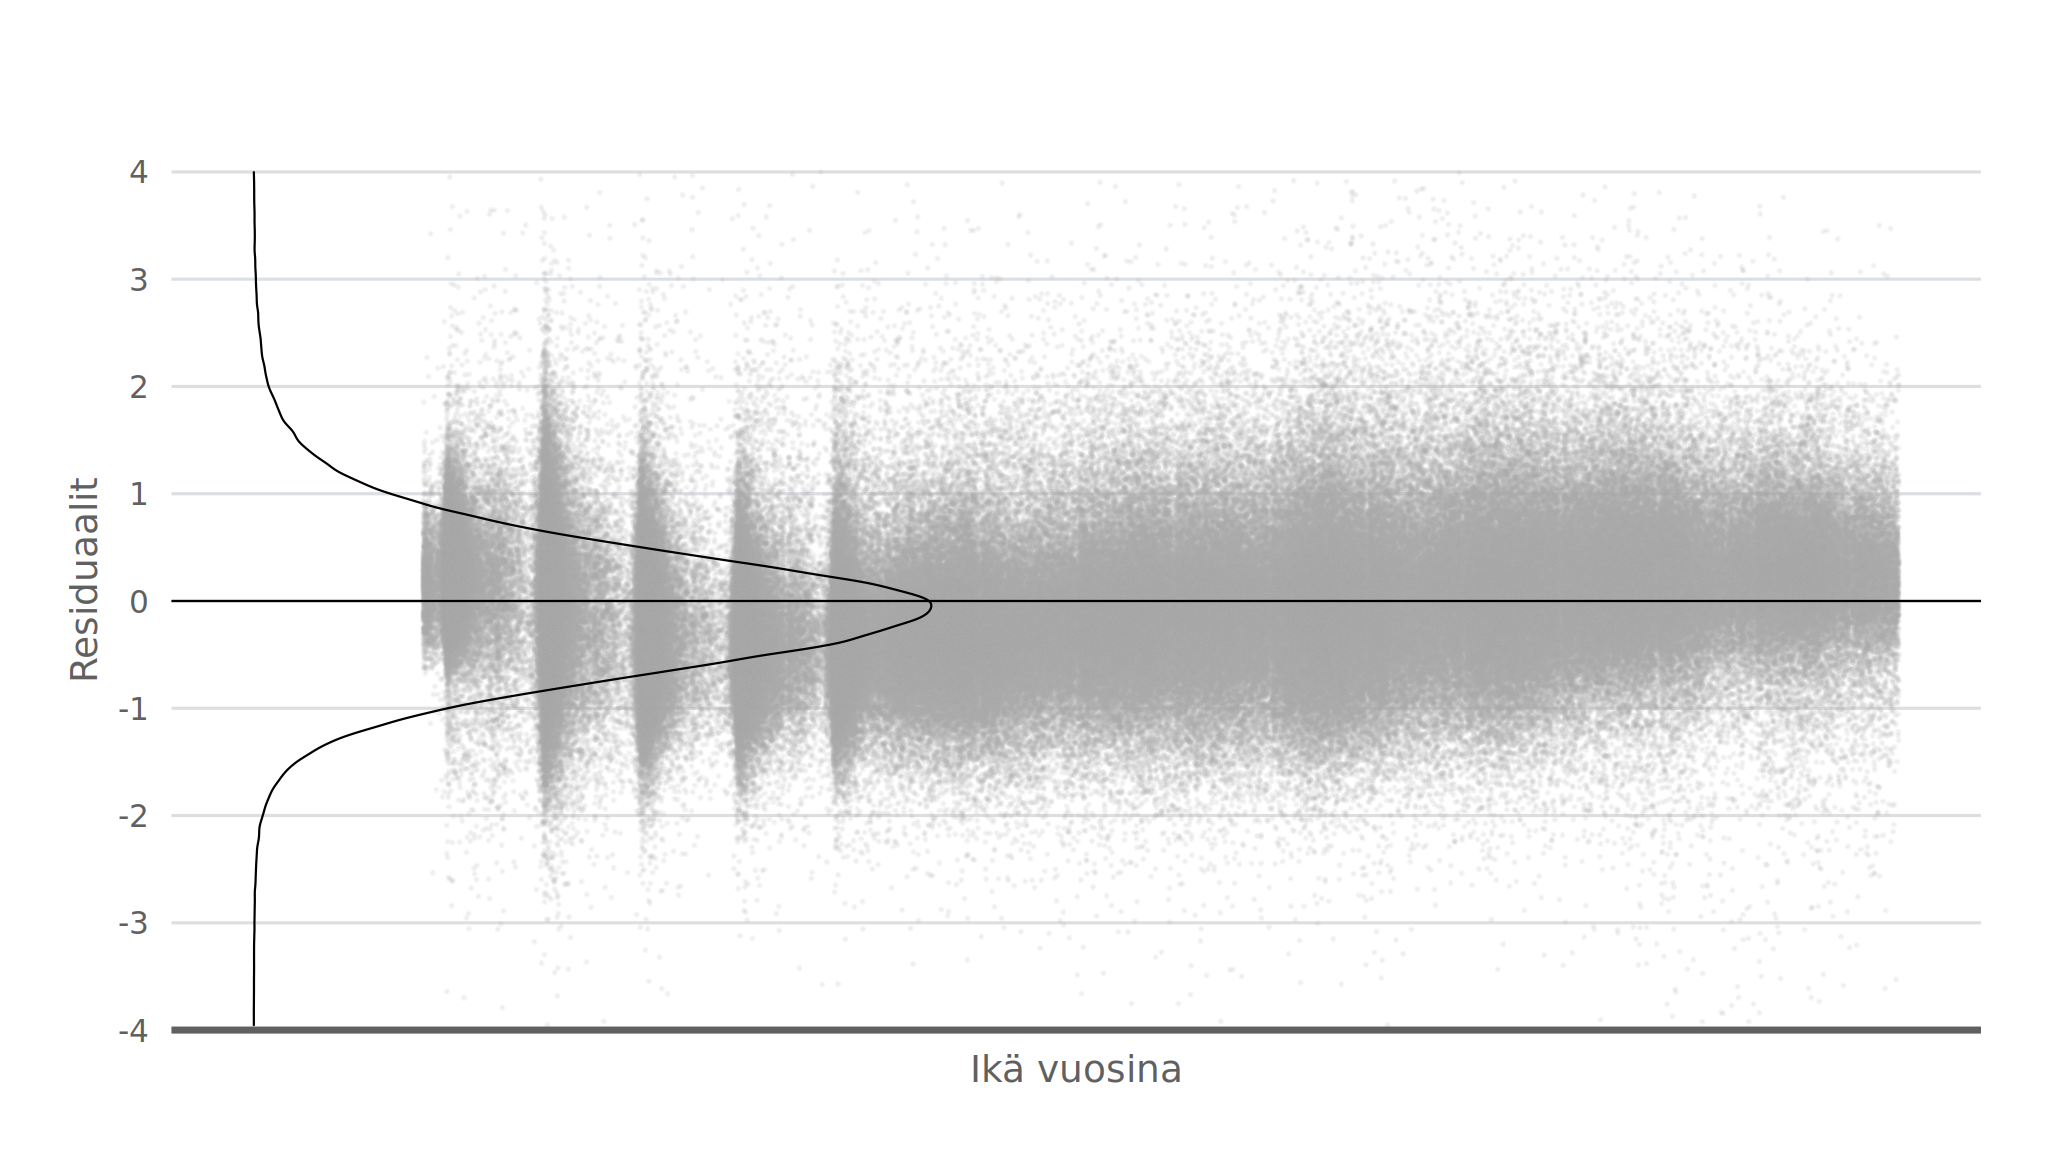
\includegraphics[scale=0.8]{kuvaajat/lme2_ika_vc_residuaalit.png}
  \caption{Satunnaisvaikutusten laajennetun mallin yksilökohtaisten mittausten Pearson-residuaalit iän suhteen ja tiheysfunktion Gaussin ydinestimaatti.}
  \label{fig:lme2_ika_vc_resid}
\end{figure}

\begin{figure}[H]
\centering
  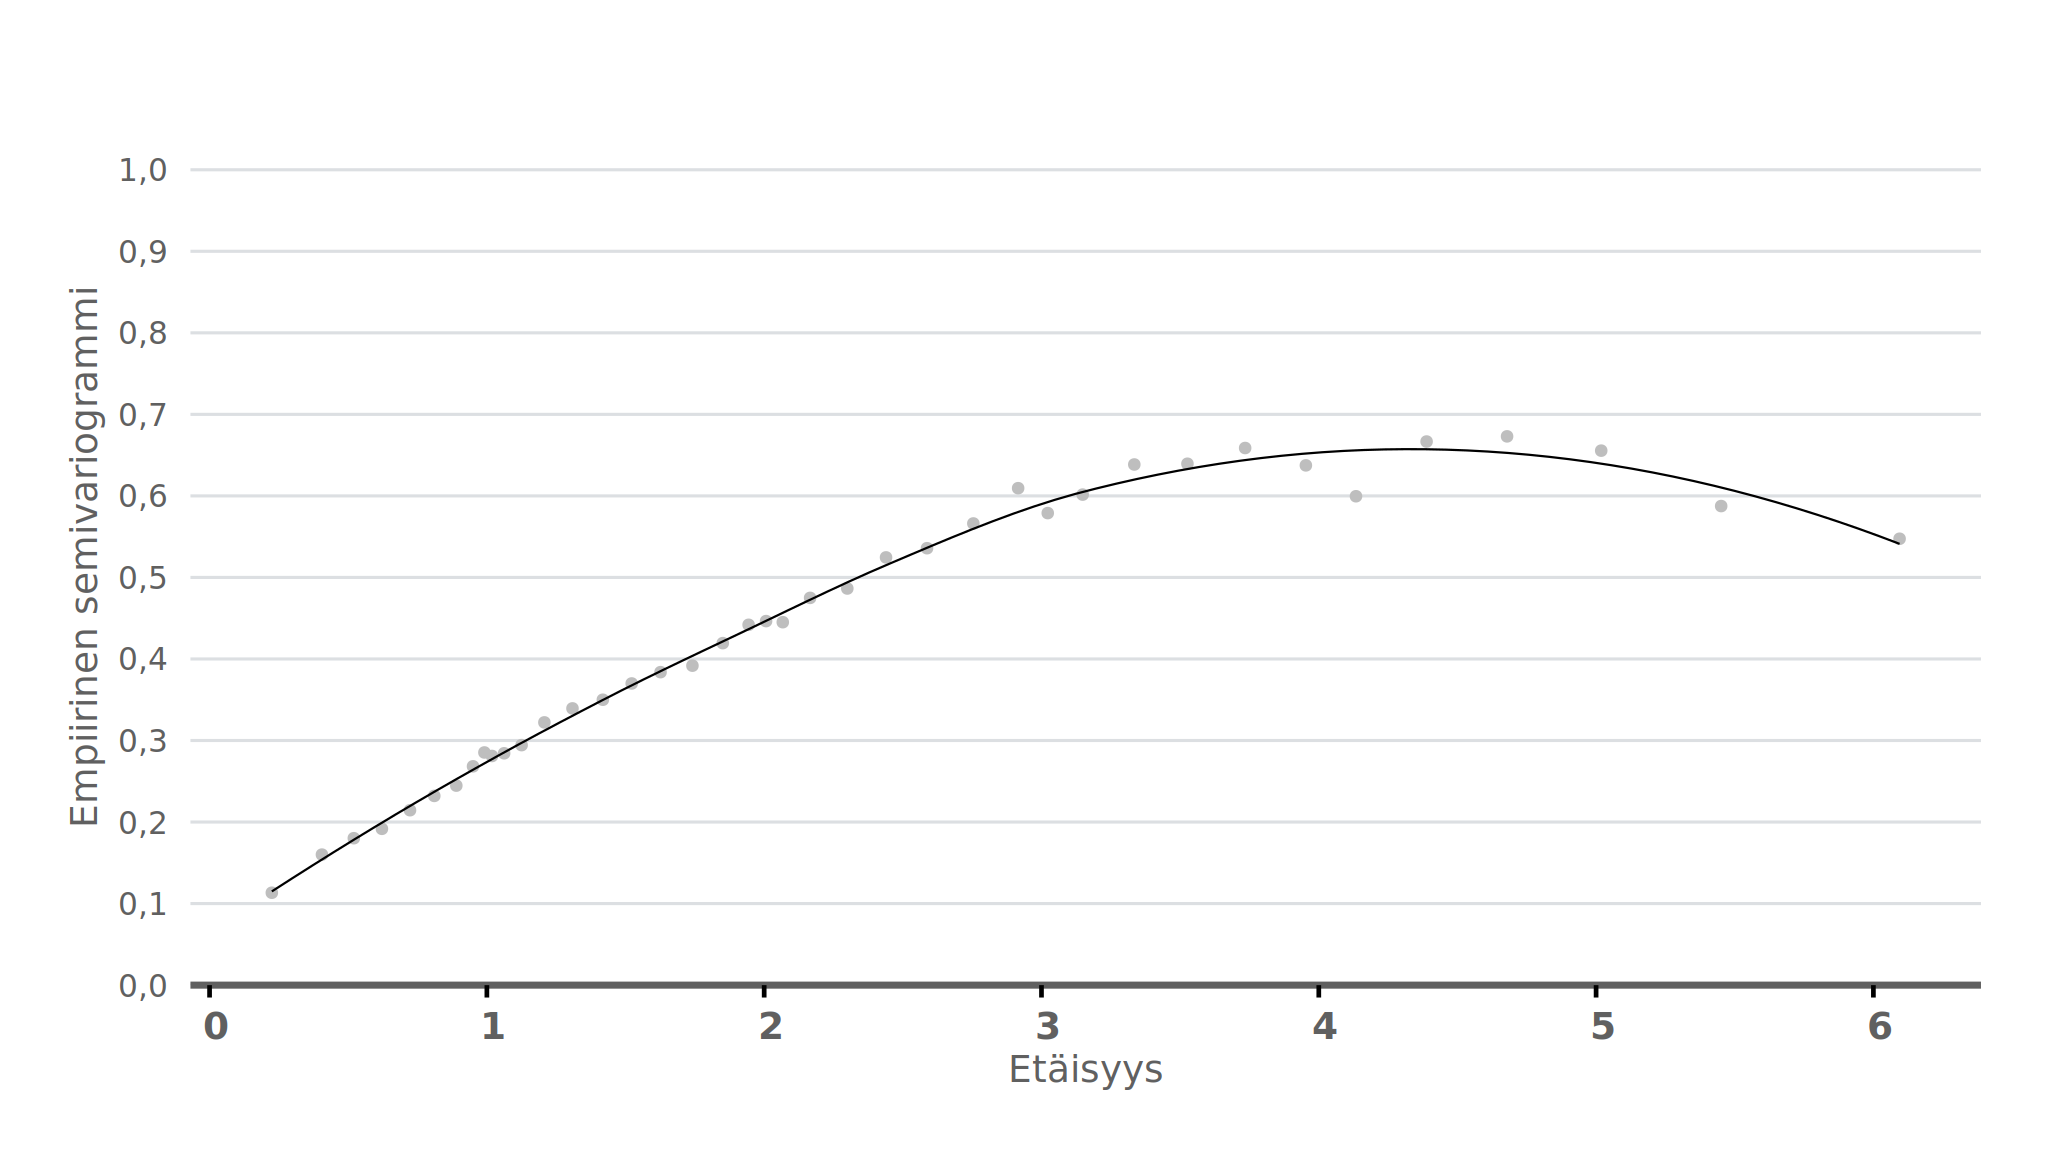
\includegraphics[scale=0.8]{kuvaajat/lme2_vc_vario.png}
  \caption{Satunnaisvaikutusten laajennetun mallin empiirinen semivariogrammi ($\hat{\gamma}$).}
  \label{fig:lme2_vc_vario}
\end{figure}

\begin{table}[H]
\centering
\begin{tabular}{lrrrrr}
\toprule
  & Estimaatti & Keskivirhe ($\text{se}$) & P & $\text{LV}_{2,5}$ & $\text{LV}_{97,5}$\\
\midrule
$\hat{\beta}_0$ & 15,428 & 0,0132 & 0,0000 & 15,402 & 15,454\\
$\hat{\beta}_1$ & -0,1564 & 0,0023 & 0,0000 & -0,1609 & -0,1519\\
$\hat{\beta}_2$ & 0,2841 & 0,0025 & 0,0000 & 0,2792 & 0,2889\\
$\hat{\beta}_3$ & -0,3179 & 0,0175 & 0,0000 & -0,3522 & -0,2835\\
$\hat{\beta}_4$ & 0,0447 & 0,0032 & 0,0000 & 0,0383 & 0,0510\\
\bottomrule
\end{tabular}
\caption{Laajennetun satunnaisvaikutusmallin $\text{LSM}_{\text{VK}}$~\ref{eq:lme2} kiinteiden vaikustusten REML-estimaatit}
\label{table:lme2vk}
\end{table}

\begin{table}[H]
\centering
\begin{tabular}{lrrrrr}
\toprule
  & Estimaatti & Keskivirhe ($\text{se}$) & P & $\text{LV}_{2,5}$ & $\text{LV}_{97,5}$\\
\midrule
$\hat{\sigma^2}_{\text{b}_{0i}}$ & 3,7878 & 1,9462 & 0 & 3,7047 & 3,8729 \\
$\hat{\sigma^2}_{\text{b}_{1i}}$ & 0,1915 & 0,4376 & 0 & 0,1884 & 0,1946 \\
$\hat{\sigma}_{\text{b}_{0i}, \text{b}_{1i}}$ & -0,6898 & - & - & - & - \\
\addlinespace
$\hat{\sigma^2}$ & 0,1611 & 0,4014 & 0 & 0,1566 & 0,1659 \\
\bottomrule
\end{tabular}
\caption{Laajennetun satunnaisvaikutusmallin $\text{LSM}_{\text{VK}}$~\ref{eq:lme2} satunnaisvaikustusten ja residuaalien varianssi-kovarianssiestimaatit. Kovarianssille ei saatavilla keskivirhettä tai luottamusvälejä (-). *Luottamusvälit arvioitu normaaliapproksimaatiolla}
\label{table:lme3vk}
\end{table}

Kiinteiden vaikutusten parametrien estimaateissa (Taulukko ~\ref{table:lme2vk}) on havaittavissa pieniä muutoksia satunnaisvaikutusten korreloimattoman ja vakiovarianssisen mallin estimaatteihin, mutta merkittävin ero luonnollisesti löytyy satunnaisvaikutusten ja residuaalien varianssi- ja kovarianssiestimaateista (Taulukko~\ref{table:lme3vk}). Vakiotermin satunnaisvaikutuksen ja residuaalivarianssin estimaatit ovat huomattavasti pienempiä.\\

Tulokset antavat vahvoja viitteitä varianssi- ja autokorrelaatiofunktioiden määrittelylle, mutta vakavastiotettavien johtopäätösten tuottamiseksi malli tulisi tarkistaa \cite{pinheiro00} esittämän laajennetun lineaarisen sekamallin määritelmän mukaiseksi.\\

Lopullista mallia etsiessämme tulemme kuitenkin hyödyntämään laajennetun mallin tuloksia viitteellisinä kontrafaktuaaleina, joihin peilaamme lopullisesta mallista saatuja tuloksia.\\

\subsubsection{Mallin parametrien karsinta}
\label{ssb:malliparamkars}

Palaamme tarkastelemaan satunnaisvaikuten mallia LSM~\ref{eq:lme2} ja arvioimme kriittisesti kiinteiden vaikutusten perusteita vertaamalla täyttä mallia kiinteille vaikutusille kriittisiin malleihin. Koska vertaamme malleja, joissa kiinteät vaikutukset eivät ole samoja, sovitamme mallit ML-menetelmällä.\\

Kriittisiksi malleksi muodostamme satunnaisvaikutusten mallin ilman kiinteää sukupuolen ja iän yhdysvaikutusta (LSM~\ref{eq:lme2.1})

\begin{equation}
\begin{split}
 \text{BMI}_{ij} = \beta_0 + \beta_1 \times \text{IKÄ}_{i0} + \beta_2 \times \text{IKÄ}_{ij} + \beta_3 \times \text{SUKUPUOLI}_{ij}\\
 + \text{b}_{0i} + \text{b}_{1i} \times \text{IKÄ}_{ij} + \epsilon_{ij},
\label{eq:lme2.1}
\end{split}
\end{equation}

sekä täysin ilman kiinteää sukupuolen vaikutusta (LSM~\ref{eq:lme2.2})

\begin{equation}
\begin{split}
 \text{BMI}_{ij} = \beta_0 + \beta_1 \times \text{IKÄ}_{i0} + \beta_2 \times \text{IKÄ}_{ij} + \text{b}_{0i} + \text{b}_{1i} \times \text{IKÄ}_{ij} + \epsilon_{ij}.
\label{eq:lme2.2}
\end{split}
\end{equation}

\cite{west14} mukaan yliparametrisoidun mallin on tarkoitus tarjota perusteet satunnaisvaikutusten määrittämiseen, mutta lopuksi tavoitteena on löytää kompromissi mahdollisimman yksinkertaisen, mutta riittävän selitysvoimaisen mallin välillä.

Vaikka täysi malli (LSM~\ref{eq:lme2}) tarjoaa viitteellisesti parhaan yhteensopivuuden aineiston suhteen, informaatiokriteerien (Taulukko~\ref{table:kriit1}) perusteella ylimääräisten kiinteiden vaikutusten säilyttämiseen ei näytä olevan perusteita.\\

\begin{table}[H]
\centering
\begin{tabular}{lrrrr}
\toprule
Malli & $df$ & $l(\bm{\beta})$ & AIC & BIC\\
\midrule
LSM~\ref{eq:lme2.2} & 7 & -729345.8 & 1458706 & 1458782\\
LSM~\ref{eq:lme2.1} & 8 & -729297.8 & 1458612 & 1458699\\
LSM~\ref{eq:lme2} & 9 & -729214.8 & 1458448 & 1458546\\
\bottomrule
\end{tabular}
\label{table:kriit1}
\end{table}

Suuresta havaintomäärän $n$ suhteesta parametrien määrään $p$ seuraten perinteiset mm. F- ja $\chi^2$ -testisuureisiin perustuvat tilastolliset testit tulkitsevat hyvinkin pienet erot merkitseviksi. \cite{burzykowski13} mukaan tilanteissa, joissa hypoteesien testausta ei katsota mielekkääksi, voidaan mallinvalinnassa hyödyntää informaatiokriteerien arviota mallin ja aineiston yleisestä yhteensopivuudesta.\\ 

Erääksi vaihtoehdoksi \cite{burzykowski13} ehdottavat myös kiinteiden vaikutusten parametrien empiiristen jakaumien simulointia esimerkiksi LOO-menetelmällä (\textit{Leave-One-Out}), jossa jakaumaa estimoidaan poistamalla yksittäisiä havaintoja, tai siirtymällä kokonaan bayesiläisiin menetelmiin.\\

Simulaatiomenetelmille ei kuitenkaan kyetyy tämän tutkielman piirissä löytämään laskennallisesti riittävän tehokasta toteutusta ja yleisesti Bayes-kehikon yhteensovittamista tutkielmassa rajattuun näkökulmaan lineaarisista sekamallesta ei katsottu tutkielman kokonaisuuden mielekkääksi.\\ 

Vahvistaaksemme päätöksen valita kiinteille vaikutuksille kriittinen malli LSM~\ref{eq:lme2.2}, pyrimme varmistumaan mallin satunnaisvaikutusten ja residuaalien jakaumaoletuksista, verraten niitä täyteen malliin LSM~\ref{eq:lme2}. Peilaamme näitä malleja myös laajennettuihin vertailumallehin $\text{LSM}_{\text{VK}}$~\ref{eq:lme2} ja $\text{LSM}_{\text{VK}}$~\ref{eq:lme2.2}, joissa on huomioitu varianssipainot ja autokorreloituneet residuaalit.\\

Yksilökohtaisten residuaalien normaalisuusoletuksen tarkistamiseen \cite{burzykowski13} suosittelevat kvantiili-kvantiilikuvaajaa (\textit{Q-Q plot}), jossa Pearsonin residuaaleja, järjestettynä pienimmästä arvosta suurimpaan, verrataan oletusjakauman teoreettisiin kvantiileihin. Kuvaajassa havaittujen arvojen tulisi asettua likimain suoralle apuviivalle, joka kulkee ensimmäisen ja kolmannen kvantiilin läpi, jotta havaitun jakauman katsotaan noudattavan oletettua jakaumaa.\\

Kuvan~\ref{fig:lme_resid_qq} mallien symmetrinen, mutta hännistä kaareutuva kuvaaja viittaa jakauman paksuhäntäisyyteen. Tämä tarkoittaa sitä, että empiirinen jakauma sisältää normaalijakaumaan nähden äärimmäisempiä arvoja \cite{pinheiro00}. Silmämääräisesti ei ole havaittavissa, että mallit $\text{LSM}_{\text{VK}}$~\ref{eq:lme2} ja $\text{LSM}_{\text{VK}}$~\ref{eq:lme2.2} tarjoaisivat huomattavaa lisäarvoa.\\

\begin{figure}[H]
\centering
\begin{subfigure}[b]{0.4\textwidth}
\centering
  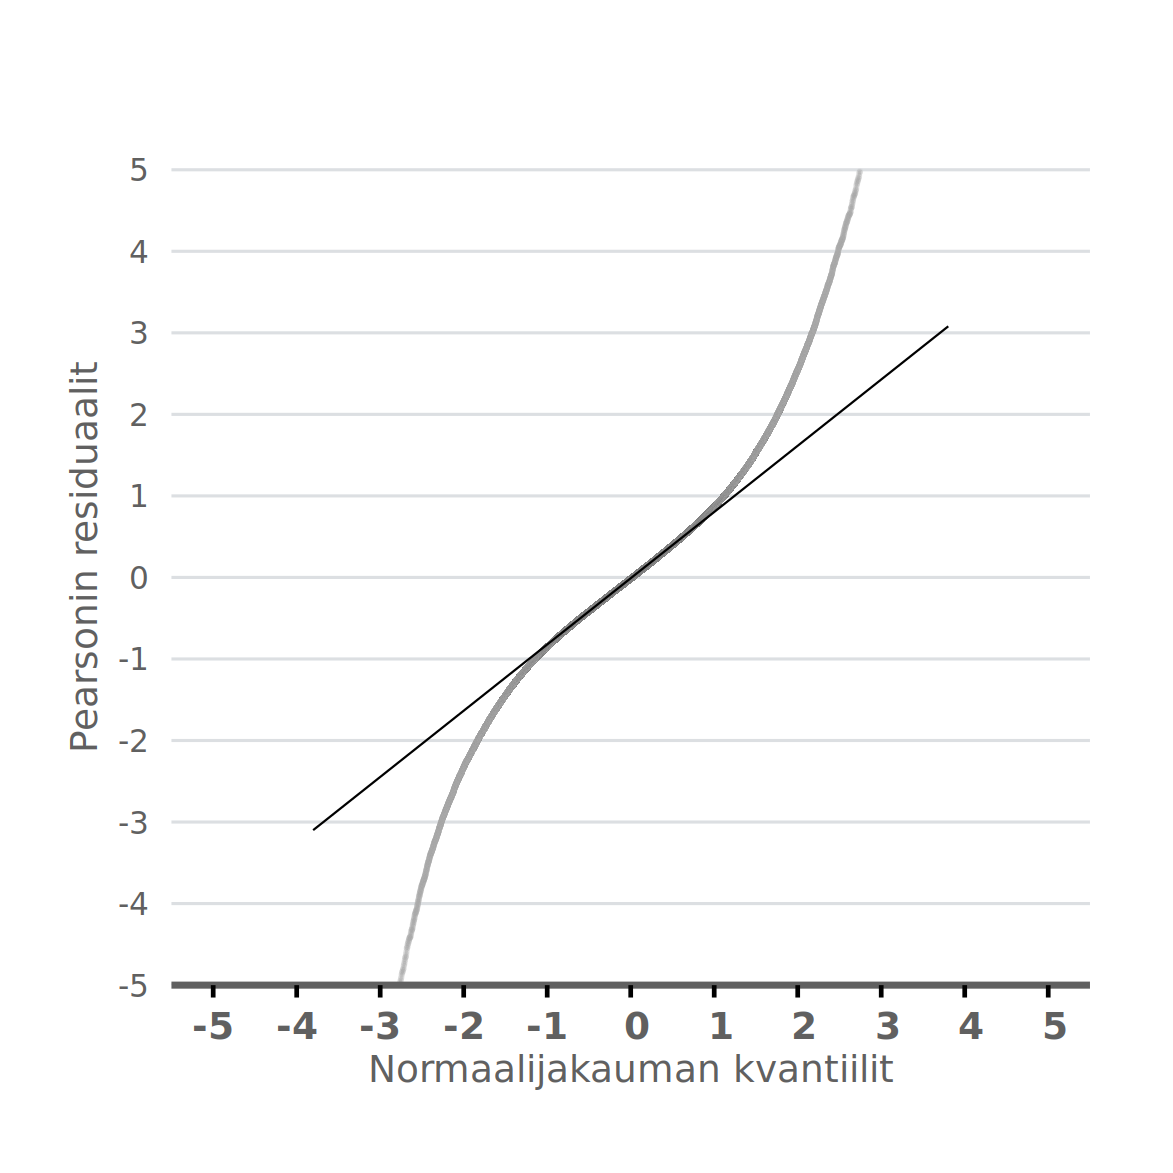
\includegraphics[width=.8\linewidth]{kuvaajat/lme3_qq.png}
  \caption{Kriittinen malli $\text{LSM}$~\ref{eq:lme2.2}}
  \label{fig:lme_krit_qq}
\end{subfigure}%
\begin{subfigure}[b]{0.4\textwidth}
\centering
  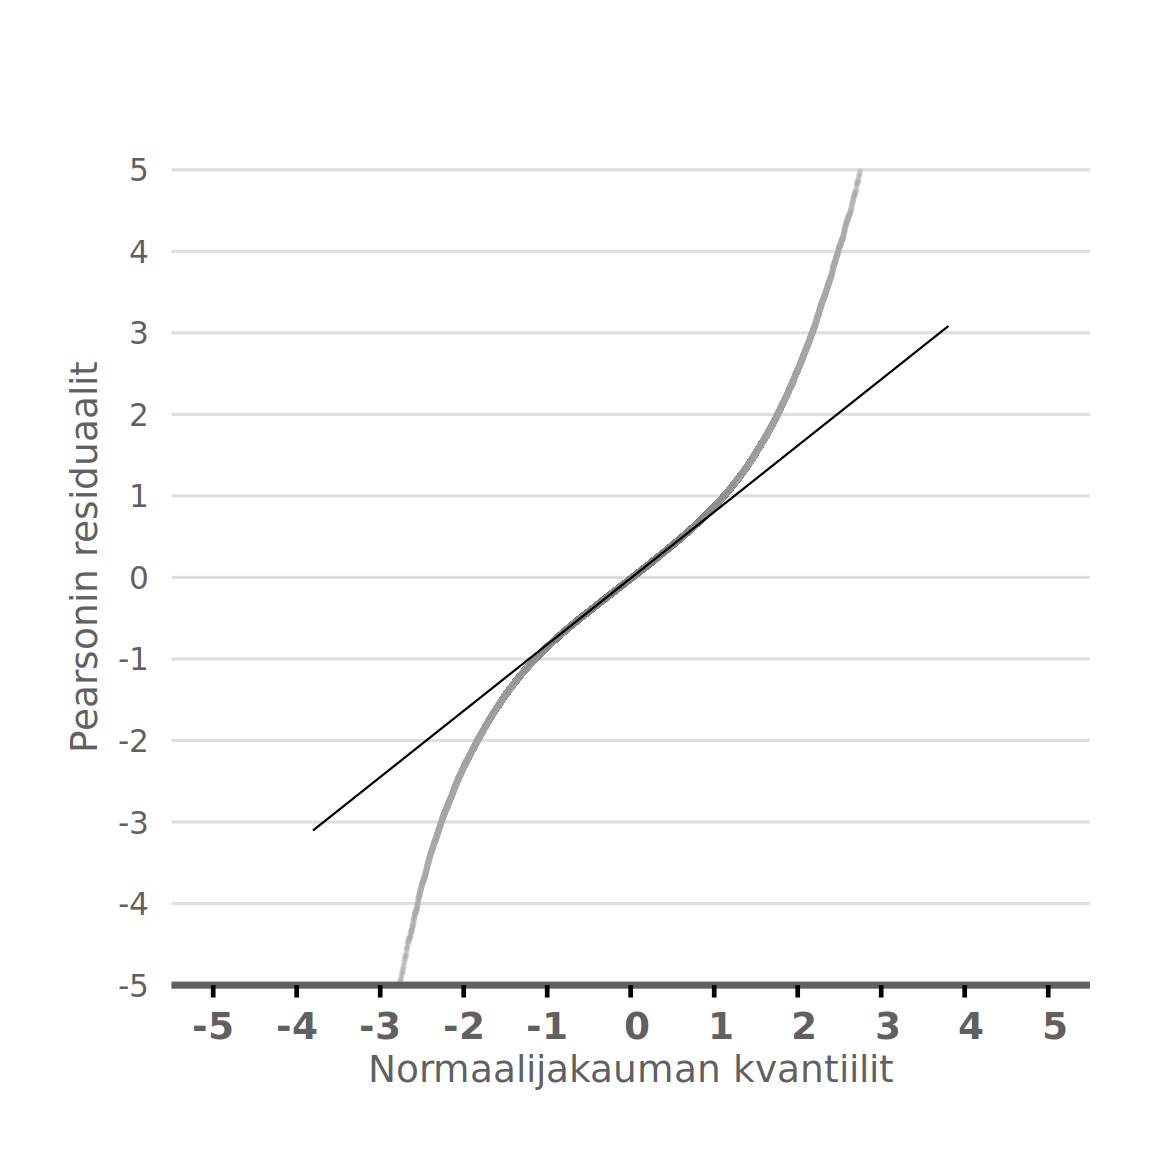
\includegraphics[width=.8\linewidth]{kuvaajat/lme3_full_qq.png}
  \caption{Täysi malli $\text{LSM}$~\ref{eq:lme2}}
  \label{fig:lme_taysi_qq}
\end{subfigure}
\begin{subfigure}[b]{0.4\textwidth}
\centering
  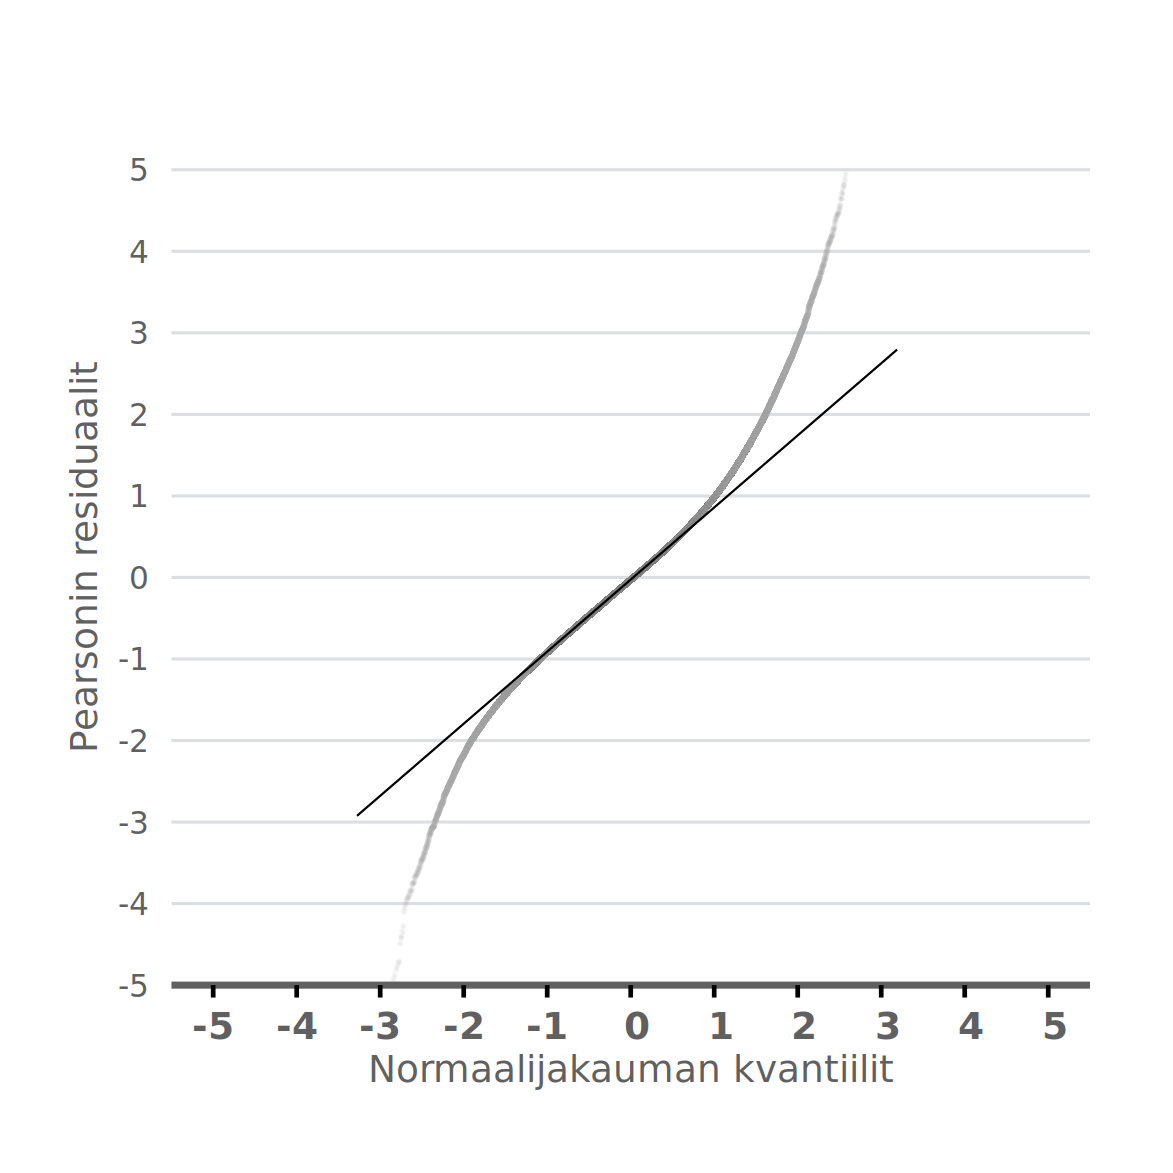
\includegraphics[width=.8\linewidth]{kuvaajat/lme3_vc_qq.png}
  \caption{Kriittinen malli $\text{LSM}_{\text{VK}}$~\ref{eq:lme2.2}}
  \label{fig:lme_vk_krit_qq}
\end{subfigure}%
\begin{subfigure}[b]{0.4\textwidth}
\centering
  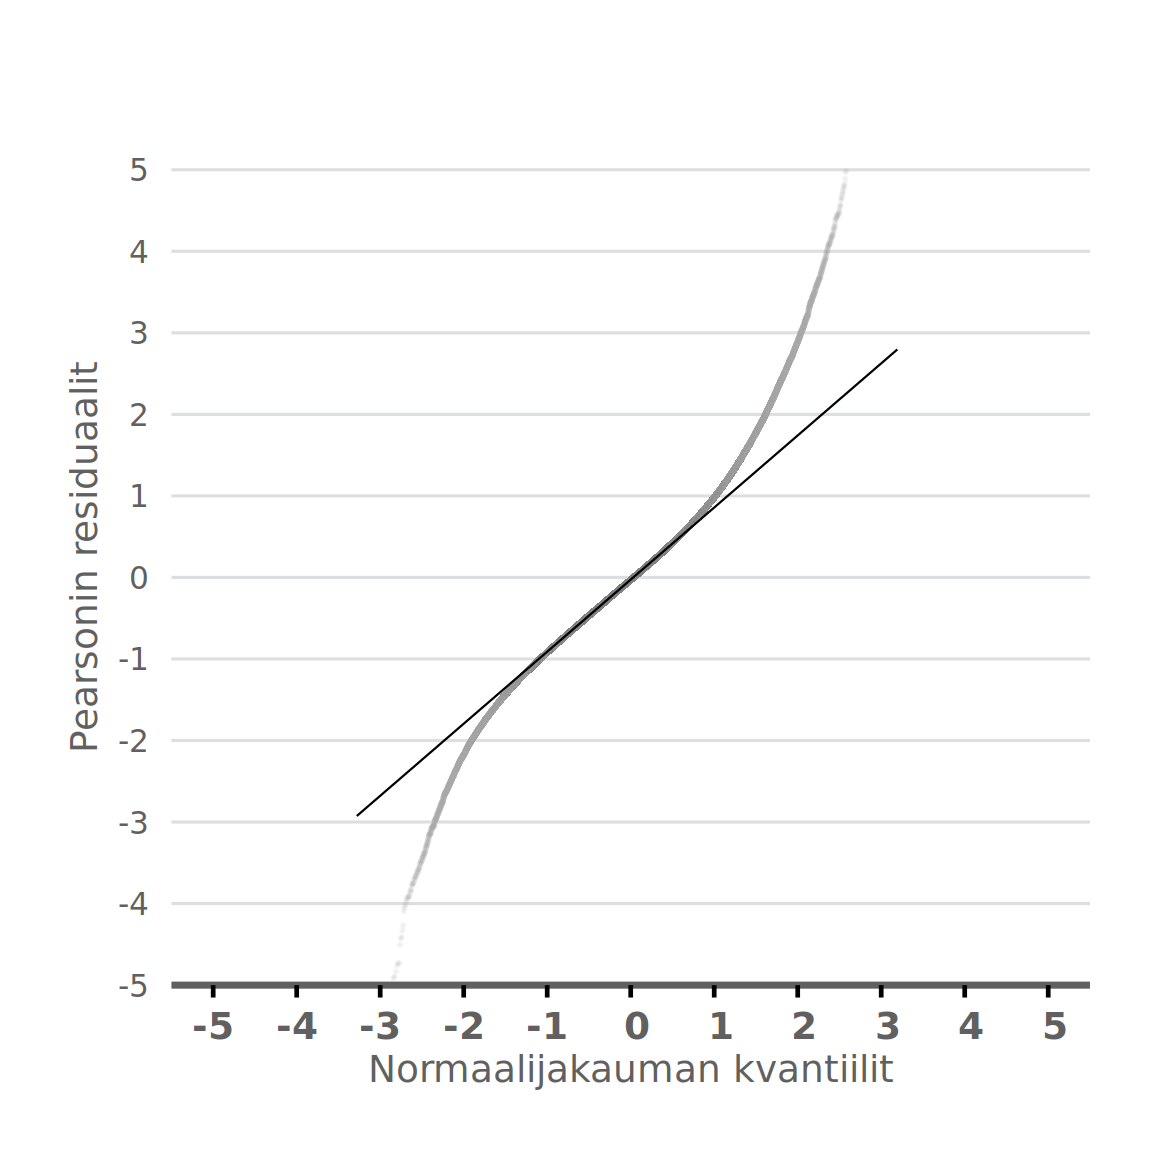
\includegraphics[width=.8\linewidth]{kuvaajat/lme3_full_vc_qq.png}
  \caption{Täysi malli $\text{LSM}_{\text{VK}}$~\ref{eq:lme2}}
  \label{fig:lme_vk_taysi_qq}
\end{subfigure}
 \caption{Kriittisen (a) ja täyden mallin (b) sekä vastaavien laajennettujen mallien (c) ja (d) kvantiili-kvantiilikuvaajat.}
   \label{fig:lme_resid_qq}
\end{figure}

Kvantiili-kvantiilikuvaajia voi varovaisin johtopäätöksin hyödyntää myös ennustettujen satunnaisvaikutusten normaalisuusoletusten tarkistamiseen, mutta \cite{burzykowski13} huomauttavat, että määritelmäänsä nojaten $\hat{\bm{b}}_i$ ei välttämättä vastaa $\bm{b}_i$ todellista jakaumaa.\\

Kuvan~\ref{fig:lme_ranef_qq} perusteella vakiotermin ennustetut satunnaisvaikutuksen vaikuttavat residuaalien tapaan likimain symmetriseltä kaikkien mallien kohdalla, mutta iän osalta jakauma on merkittävän vino. Laajennetun mallin \\

\begin{figure}[H]
\centering
\begin{subfigure}[b]{0.4\textwidth}
\centering
  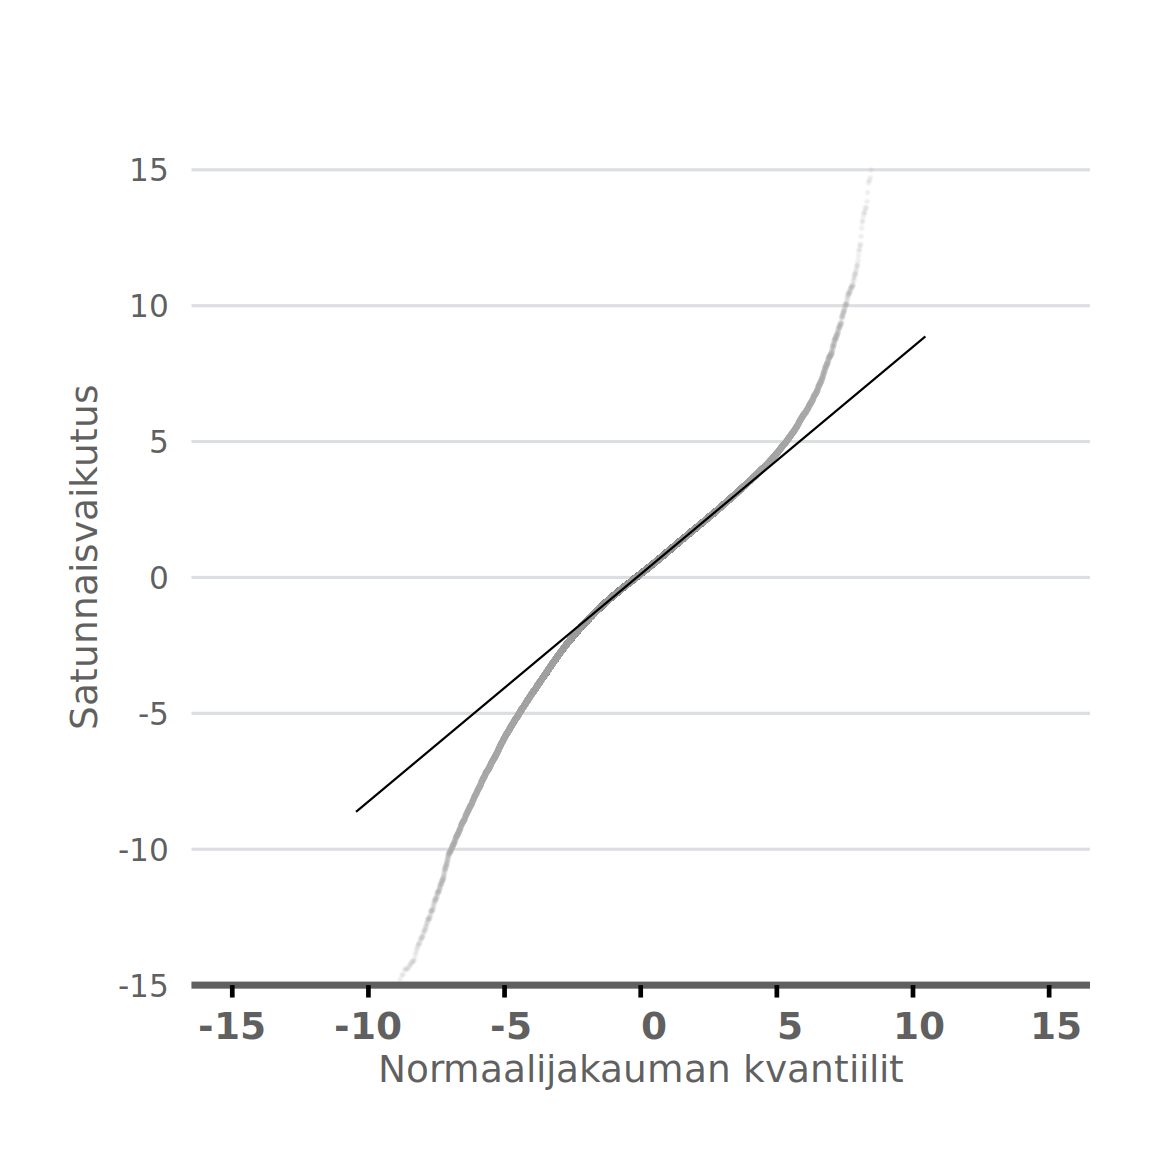
\includegraphics[width=.8\linewidth]{kuvaajat/lme3_qq_ranef_int.png}
  \caption{$\text{LSM}$~\ref{eq:lme2.2} (Vakiotermi)}
  \label{fig:lme_krit_int_qq}
\end{subfigure}%
\begin{subfigure}[b]{0.4\textwidth}
\centering
  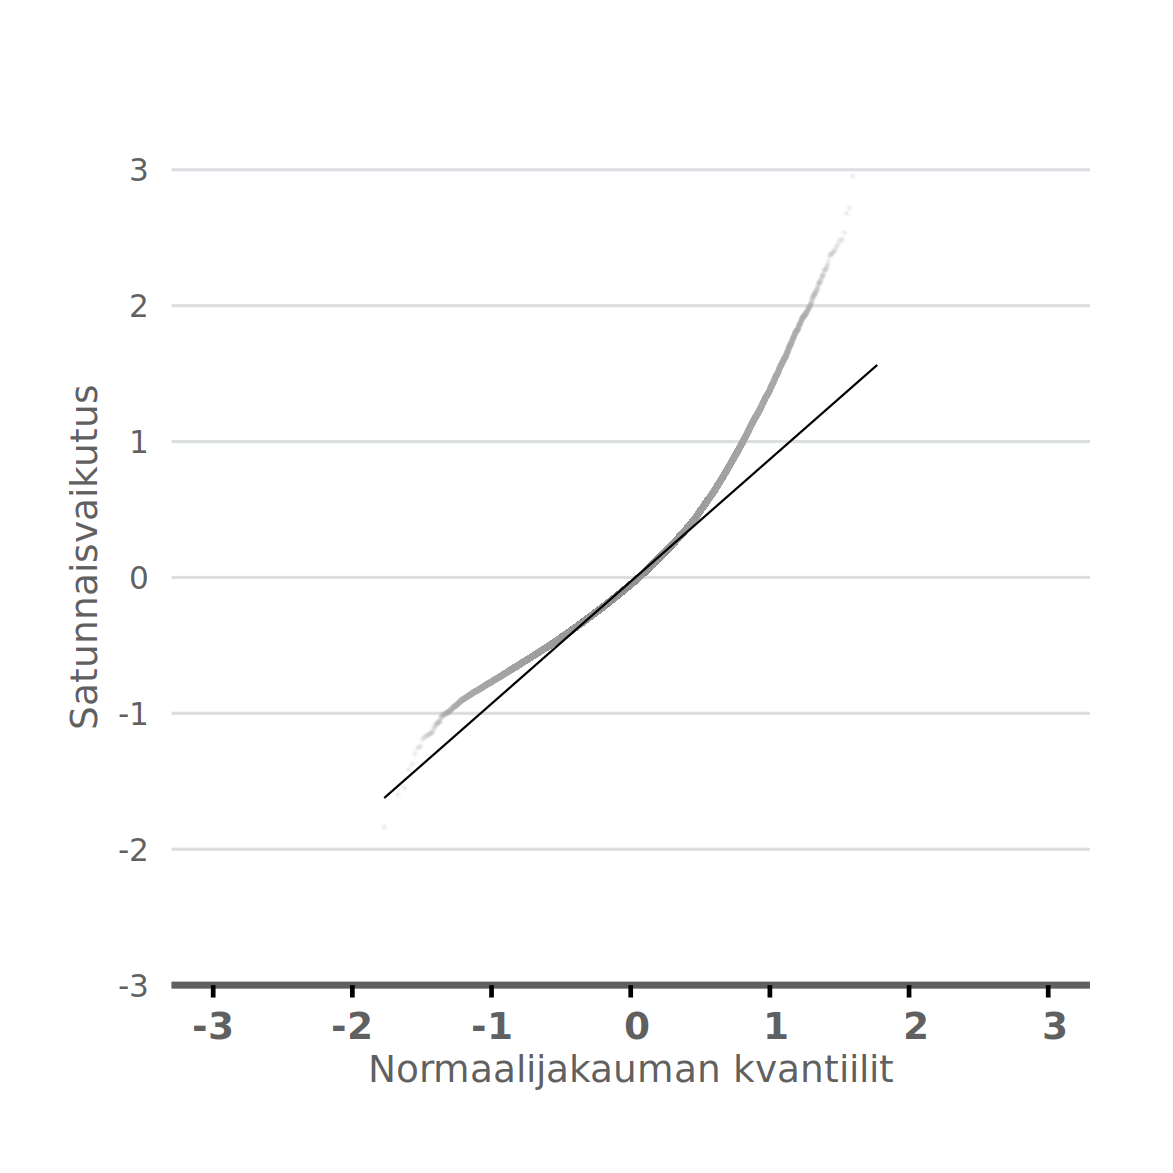
\includegraphics[width=.8\linewidth]{kuvaajat/lme3_qq_ranef_ika.png}
  \caption{$\text{LSM}$~\ref{eq:lme2.2} (Ikä)}
  \label{fig:lme_krit_ika_qq}
\end{subfigure}
\begin{subfigure}[b]{0.4\textwidth}
\centering
  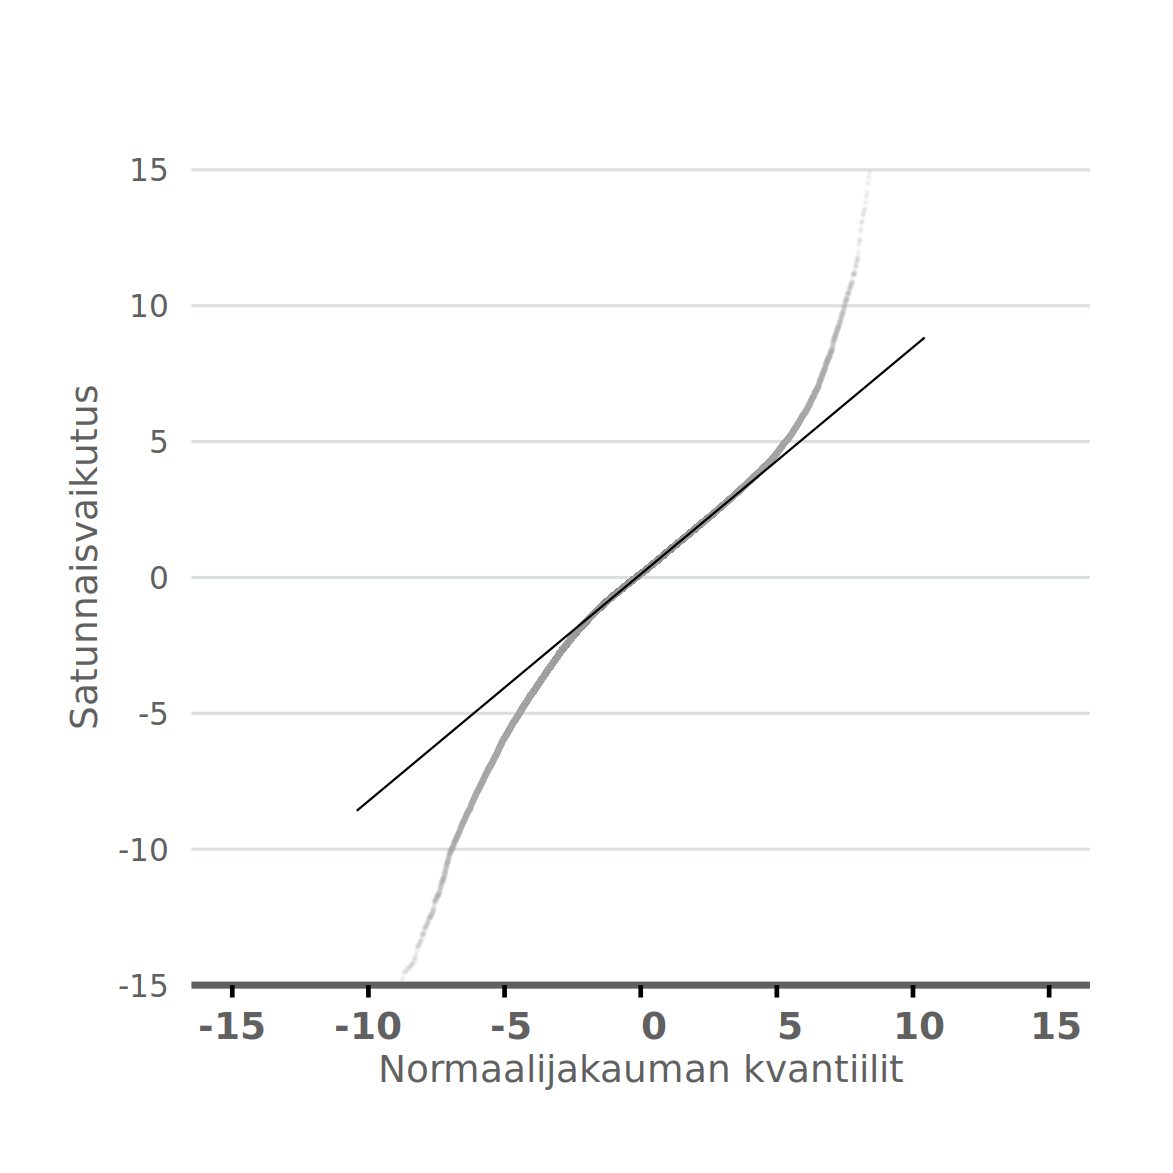
\includegraphics[width=.8\linewidth]{kuvaajat/lme3_full_qq_ranef_int.png}
  \caption{$\text{LSM}$~\ref{eq:lme2} (Vakiotermi)}
  \label{fig:lme_taysi_int_qq}
\end{subfigure}%
\begin{subfigure}[b]{0.4\textwidth}
\centering
  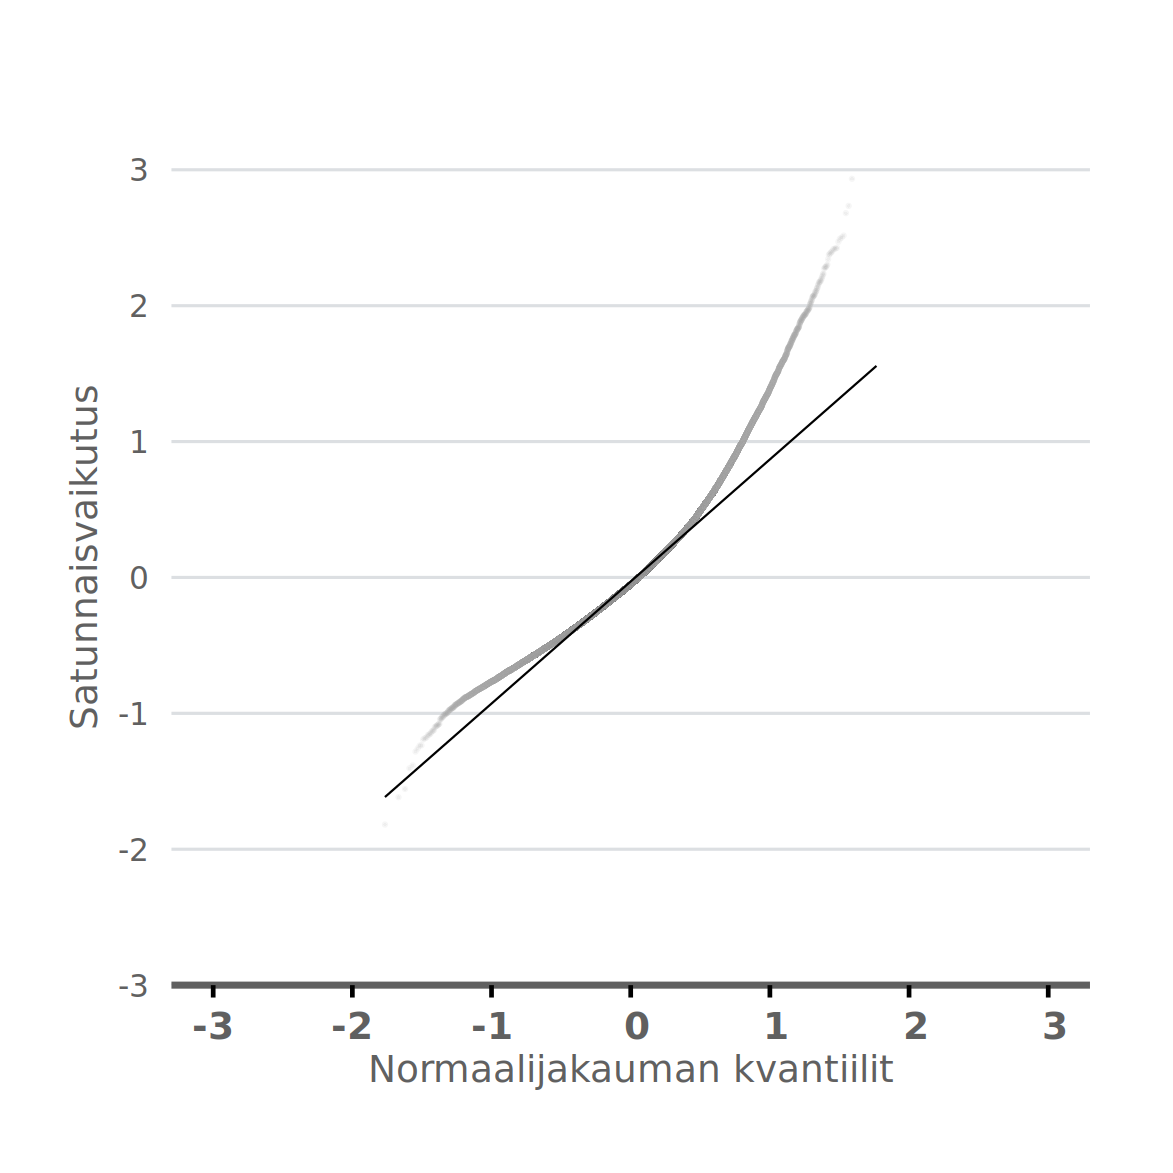
\includegraphics[width=.8\linewidth]{kuvaajat/lme3_full_qq_ranef_ika.png}
  \caption{$\text{LSM}$~\ref{eq:lme2} (Ikä)}
  \label{fig:lme_taysi_ika_qq}
\end{subfigure}
\begin{subfigure}[b]{0.4\textwidth}
\centering
  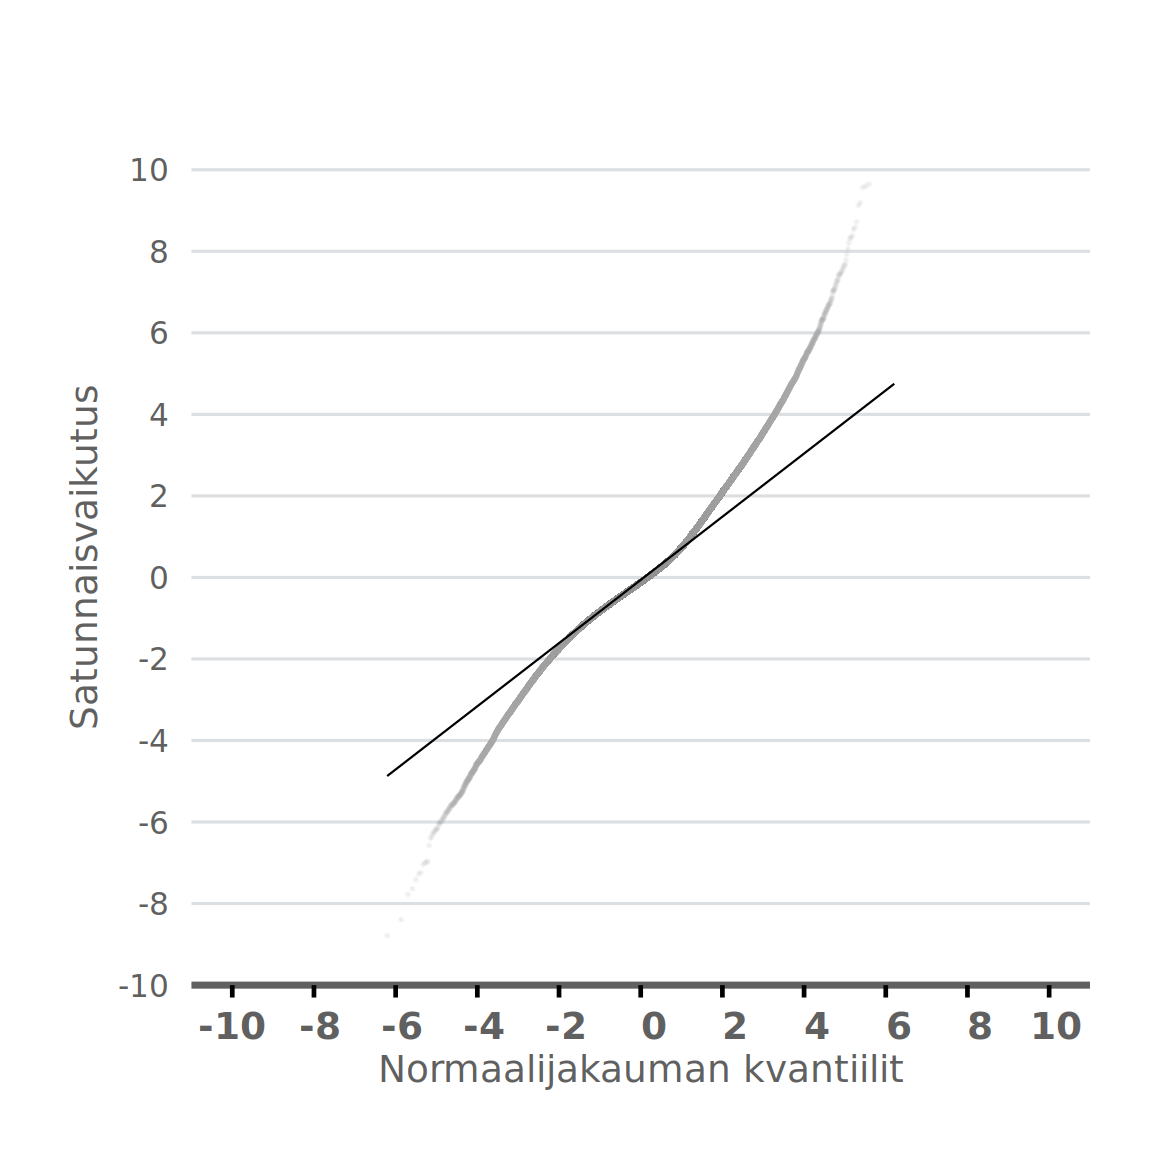
\includegraphics[width=.8\linewidth]{kuvaajat/lme3_vc_qq_ranef_int.png}
  \caption{$\text{LSM}_{\text{VK}}$~\ref{eq:lme2.2} (vakiotermi)}
  \label{fig:lme_vk_krit_int_qq}
\end{subfigure}%
\begin{subfigure}[b]{0.4\textwidth}
\centering
  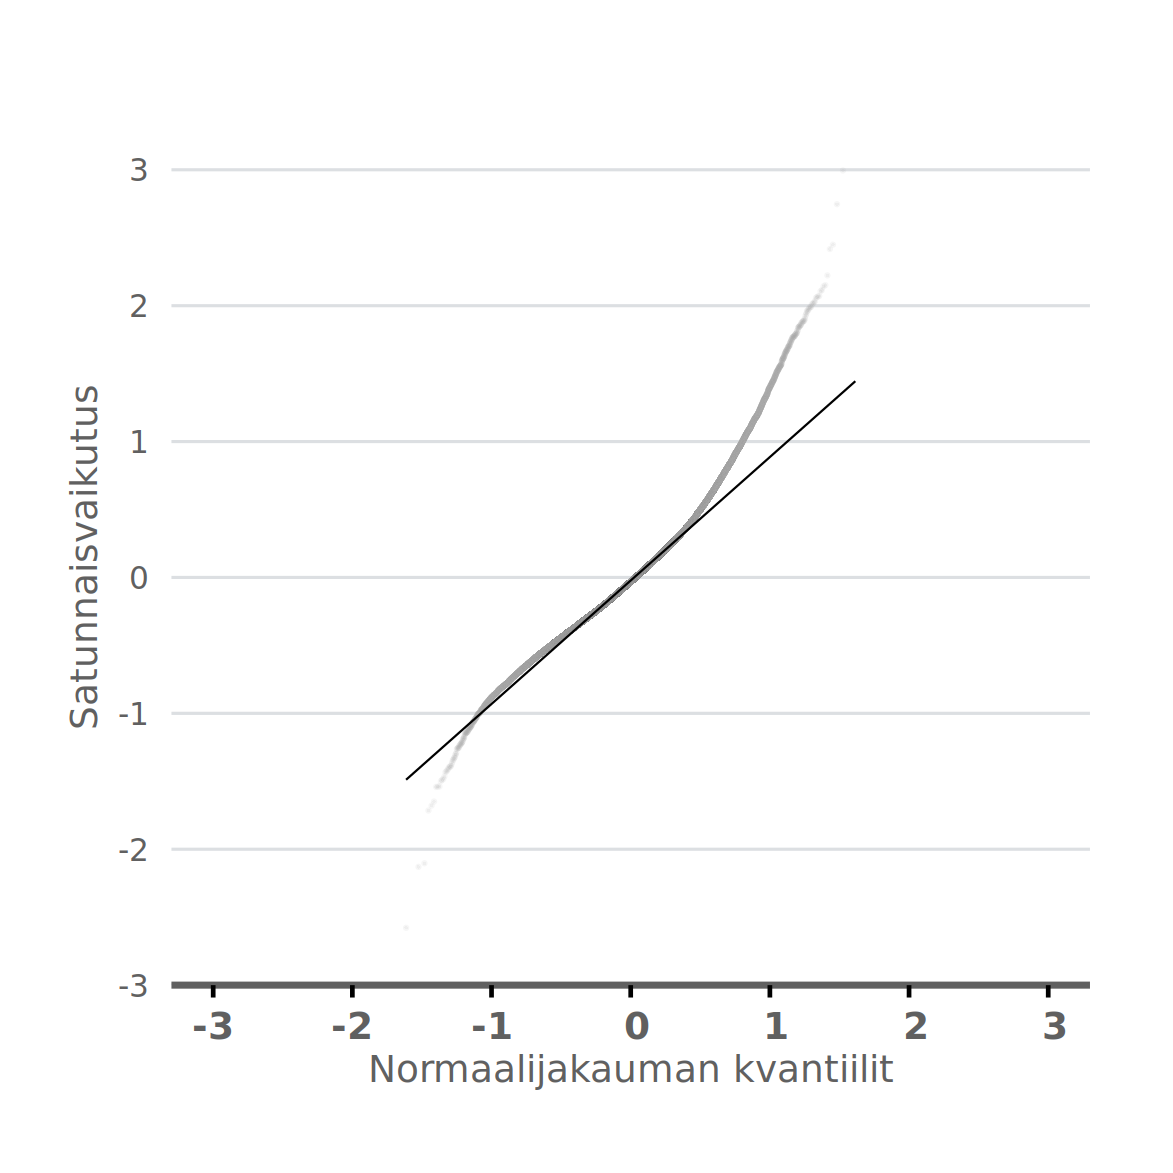
\includegraphics[width=.8\linewidth]{kuvaajat/lme3_vc_qq_ranef_ika.png}
  \caption{$\text{LSM}_{\text{VK}}$~\ref{eq:lme2.2} (Ikä)}
  \label{fig:lme_vk_krit_ika_qq}
\end{subfigure}
\begin{subfigure}[b]{0.4\textwidth}
\centering
  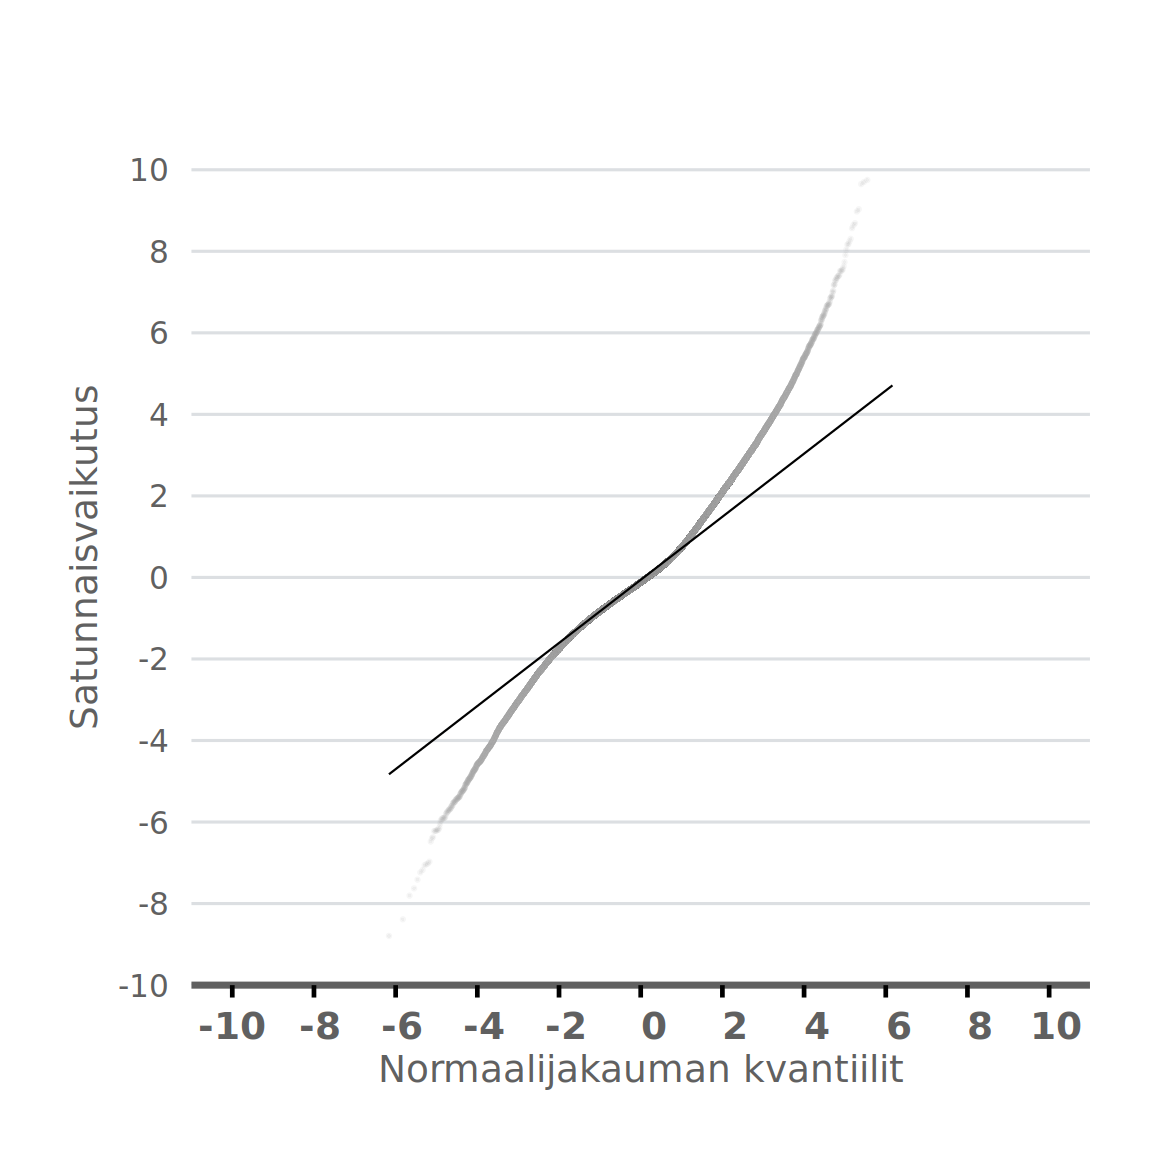
\includegraphics[width=.8\linewidth]{kuvaajat/lme3_full_vc_qq_ranef_int.png}
  \caption{$\text{LSM}_{\text{VK}}$~\ref{eq:lme2} (Vakiotermi)}
  \label{fig:lme_vk_taysi_int_qq}
\end{subfigure}%
\begin{subfigure}[b]{0.4\textwidth}
\centering
  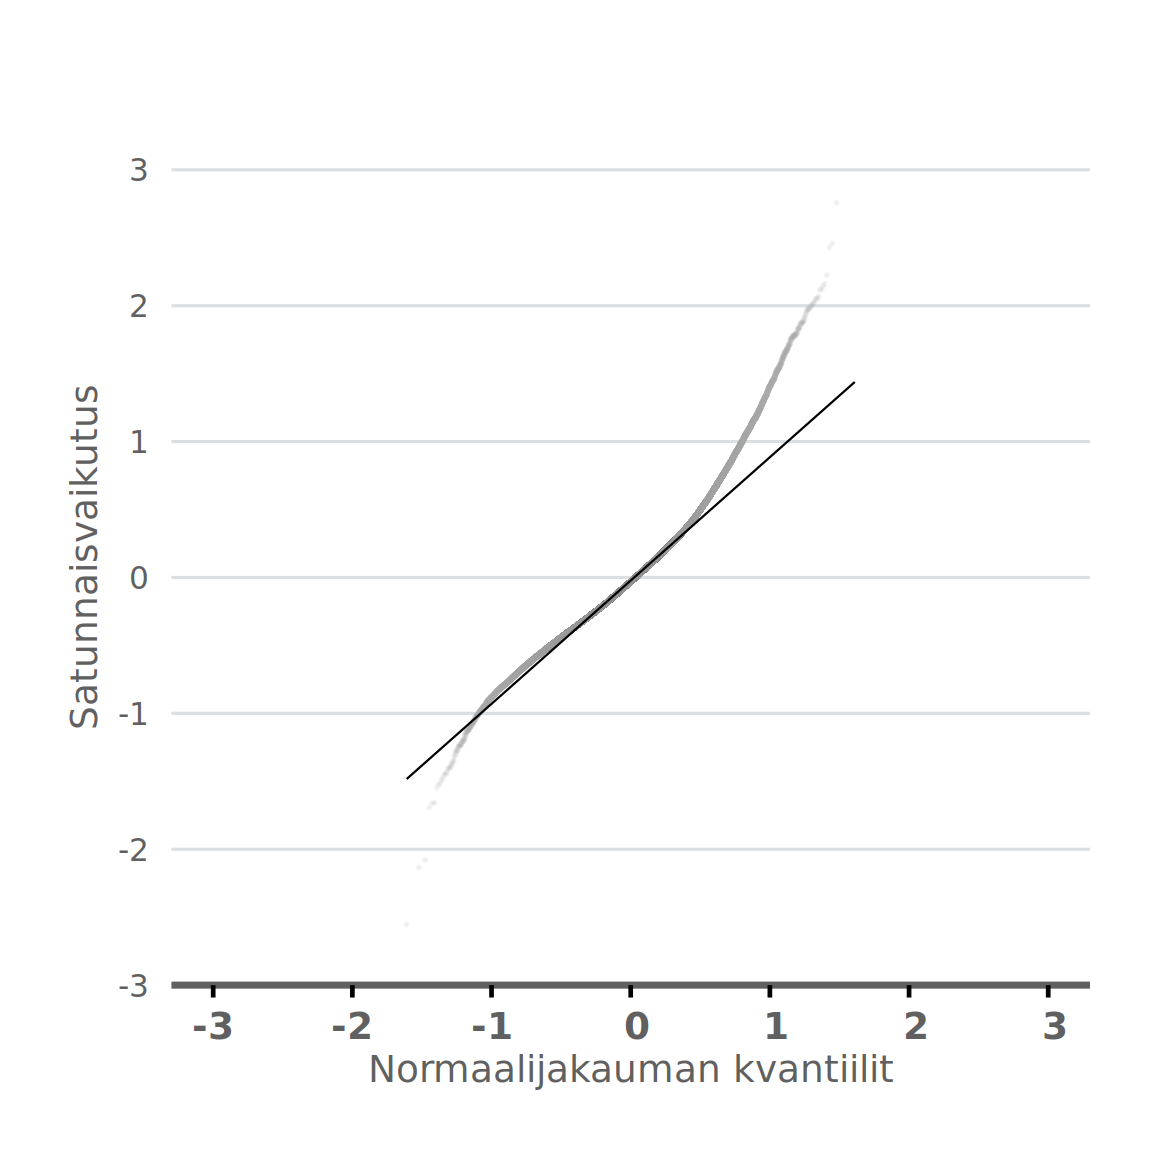
\includegraphics[width=.8\linewidth]{kuvaajat/lme3_full_vc_qq_ranef_ika.png}
  \caption{$\text{LSM}_{\text{VK}}$~\ref{eq:lme2} (Ikä)}
  \label{fig:lme_vk_taysi_ika_qq}
\end{subfigure}
 \caption{Kriittisen (a), (b) ja täyden mallin (c), (d) sekä vastaavien laajennettujen mallien (e),(f) ja (g),(h) vakiotermin ja iän ennustettujen satunnaisvaikutusten kvantiili-kvantiilikuvaajat.}
   \label{fig:lme_ranef_qq}
\end{figure}

Viimeiseksi tarkastelemme 

KIINTEILLE VAIKUTUKSILLE KRIITTINEN VK MALLI RESIDUAALIONGELMAT -- POIS

\subsubsection{Lopullinen malli}

LAIRWARE MALLIN MUODOSTAMINEN ESTIMOIDUISTA MATRIISEISTA

PUUTTEET JA KEHITYSKOHTEET

YKSILÖKOHTAISET USKOTTAVUUSKONTRIBUUTIOT - LOO-MENELMÄ VOISI ANTAA VIITTEITÄ DATAA GENEROIVASTA PROSESSISTA

\section{Johtopäätökset}

% --- References ---

\nocite{*}
% one of these or  ...
%\bibliographystyle{plain}
%\bibliographystyle{acm}
%\bibliographystyle{ieeetr}
\bibliographystyle{apalike}

\bibliography{references}

\lastpage

\appendices

\pagestyle{empty}

\internalappendix{1}{Tulokset ja taulukot}

% Table created by stargazer v.5.2.2 by Marek Hlavac, Harvard University. E-mail: hlavac at fas.harvard.edu
% Date and time: ti, touko 05, 2020 - 20.10.08
\begin{table}[!htbp] \centering 
  \caption{} 
  \label{} 
\begin{tabular}{@{\extracolsep{5pt}}lcc} 
\\[-1.8ex]\hline 
\hline \\[-1.8ex] 
 & \multicolumn{2}{c}{\textit{Dependent variable:}} \\ 
\cline{2-3} 
\\[-1.8ex] & \multicolumn{2}{c}{bmi} \\ 
\\[-1.8ex] & (1) & (2)\\ 
\hline \\[-1.8ex] 
 ika\_alku\_i & $-$0.173$^{***}$ & $-$0.174$^{***}$ \\ 
  & (0.002) & (0.002) \\ 
  & & \\ 
 ika & 0.404$^{***}$ & 0.383$^{***}$ \\ 
  & (0.002) & (0.002) \\ 
  & & \\ 
 sukupfF &  & $-$0.361$^{***}$ \\ 
  &  & (0.022) \\ 
  & & \\ 
 ika:sukupfF &  & 0.043$^{***}$ \\ 
  &  & (0.003) \\ 
  & & \\ 
 Constant & 14.440$^{***}$ & 14.625$^{***}$ \\ 
  & (0.014) & (0.018) \\ 
  & & \\ 
\hline \\[-1.8ex] 
Observations & 421,660 & 421,660 \\ 
Log Likelihood & $-$729,345.800 & $-$729,214.800 \\ 
Akaike Inf. Crit. & 1,458,706.000 & 1,458,448.000 \\ 
Bayesian Inf. Crit. & 1,458,782.000 & 1,458,546.000 \\ 
\hline 
\hline \\[-1.8ex] 
\textit{Note:}  & \multicolumn{2}{r}{$^{*}$p$<$0.1; $^{**}$p$<$0.05; $^{***}$p$<$0.01} \\ 
\end{tabular} 
\end{table} 

\end{document}

% NOTES & EXTRA

% MARIAN KORJAUKSET

% CITE STYLES
%\cite{Rao03}
%\cite{Bivand08}
%\citealt{Rao03}
%\citet{Bivand08}
%\citep{Bivand08}
%\citep[p.~99]{Bivand08}
%\citep[e.g.][]{Bivand08}
%\citep[e.g.][p.~99]{Casella02}
%\citeauthor{Bivand08}
%\citeyear{Bivand08}
